% Example template for using the unmeethesis style
% This example is for a Master's candidate in Mathematics
% It contains examples of front matter and most sections that the
% typical graduate student would need to include
% By: N. Doren 02/10/00
%     Minor mods by N. Doren 08/26/11

% Use the following specification for BOTTOM page numbering:
\documentclass[botnum, fleqn]{unmeethesis}
                 % OR
% Use the following specification for TOP page numbering:
% \documentclass[fleqn]{unmeethesis}
\usepackage{graphicx}
\usepackage{caption}
\usepackage{lscape}
\usepackage{rotating}
\usepackage{multirow}
\usepackage{textcomp}
%\usepackage[linesnumbered,algoruled,boxed,lined]{algorithm2e}
\usepackage[chapter]{algorithm}
\usepackage{subcaption}
\usepackage{algorithm}
\usepackage{algpseudocode}
\renewcommand{\algorithmicrequire}{\textbf{Input:}}
\renewcommand{\algorithmicensure}{\textbf{Output:}}
\usepackage{hyperref}
\hypersetup{
	colorlinks=true,
	linkcolor=black,
	filecolor=magenta,      
	urlcolor=blue,
}
\graphicspath{ {../Images/} }

\begin{document}

\frontmatter

% Uncomment the next command if you see weird paragraph spacing:
% That is, if you see paragraphs float with lots of white space
% in between them:

% \setlength{\parskip}{0.30cm}


\title{Detection of Pheromone Laying Event in Foraging Data of Harvester Ants Using Change Point Analysis Method}

\author{Safeeul Bashir Safee}

\degreesubject{M.S., Computer Science}

\degree{Master of Science \\ Computer Science}

\documenttype{Thesis}

\previousdegrees{B.Sc., Chittagong University of Engineering \& Technology, 2011}

\date{May, \thisyear}

\maketitle

%\makecopyright
%Copyright page is no longer necessary D. Murrell

\begin{dedication}
   To my parents and my elder brother for their support,
   encouragement and the Corvette they're giving me for graduation. \\[3ex]
\end{dedication}

\begin{acknowledgments}
   \vspace{1.1in}
  I would like to thank my thesis supervisor Professor Dr. Melanie E. Moses, for her enormous support for selecting the topic to study. Without her guidance, it would have been a tough journey for me in this field. I would also like to thank Dr. Tatiana P. Flanagan for her initial guidance to me for this topic. My heart full of gratitude to Professor Dr. Abdullah Mueen for his guidance towards my degree. 
  I am thankful to all the members of Moses Biological Computation Lab for their suggestions towards my research. 
\end{acknowledgments}

\maketitleabstract %(required even though there's no abstract title anymore)

\begin{abstract}
 Communication is an important factor in the foraging performance of
 social insects, like ants. During foraging, ants keep track of the food
 sources by using memory (site fidelity) or communicating it through pheromones. Previous field experiments showed that the rate of seed collection depends on the distribution of food in the environment. If food is spatially clustered, then ants recruit nest mates to collect from large clusters. However, we don't know when the recruitment occur. To explore this question, we analyzed foraging rates on different sizes of piles in the simulation.  Using a power law distribution to arrange seeds in piles of different sizes, we observed that for significantly large piles of seeds, the ants take more time to discover a pile, but once discovered, seeds are collected at an increased rate from that pile. We also observed that ants may repeatedly lose track of found piles and then re-find them. Using change point analysis on seed intake time series, we were able to trace the discovery of piles by detecting changes in the foraging rate.  We use simulations to determine how to correlate change points with recruitment events, and then use that relationship to infer when recruitment occurs in field data.
\clearpage %(required for 1-page abstract)
\end{abstract}
\tableofcontents
\listoffigures
\listoftables
\listofalgorithms
\addtocontents{loa}{\def\string\figurename{Algorithm}}
\begin{glossary}{Longest  string}
	\item[GA]
	Genetic Algorithm
	\item[CPFA]
	Central Place Foraging Algorithm
\end{glossary}
\mainmatter
\chapter{Introduction}
Social insects are basically species that lives in colonies and manifest three characteristics \cite{SocialInsect}. a. Group integration\cite{anderson2001individual}, b. Division of labor\cite{beshers2001models} and c. Overlapping of generations\cite{wilson2005eusociality}. These creatures have survived many mass level extinction events that happened in the earth. Millions of years of genetic evolution to survive in the hostile environment helped them to adapt to the environment and master the strategies of survival.  \par
Their strategies to avoid congestion and optimize their movements to move or forage in most efficient ways without any central authorities has attracted so many researchers and scientists over the centuries\cite{narzt2010self}. As a result, we got a new branch of science which is called myrmecology. In modern computer science, machine learning\cite{dorigo1997ant}, complex interactive networks\cite{he2011ant}, parallel computing\cite{bonabeau2000inspiration} and many other topics have been inspired by the studying and modeling of ants. \par
Harvester ants are social insects. They forage from the environment. Most of their foraging activities are during the morning or in the evening sessions. And their foraging activity is at the top during the summer\cite{hobbs1985harvester, whitford1975factors}.  In this study, we will mostly talk about \textit{Progonomyrmex} species which are group foragers\cite{whitford1978foraging}. Foraging activities of harvester ants including \textit{Progonomyrmex sp.} depends on many factors like environment temperature, light, and availability of seeds\cite{whitford1975factors}.\par 
Social insects like ants use pheromone to communicate with each other to perform their daily activities which also includes foraging\cite{jackson2006communication}.
  The previous study has shown that they follow three strategies to forage from the environment\cite{flanagan2012quantifying}. Ants use memory to remember the location of the food source. They communicate with other ants using pheromone and they perform the random walk in the spatial dimension in search of food.\par 
  Foraging of ants from a particular food source depends mostly on the how  food is distributed in the environment\cite{traniello1989foraging}. To analyze the foraging strategies of ants field experiments has been conducted on three species of Pogonomyrmex desert harvester ants. Foods were distributed among the nest in different distributions to observe the effect of food density on foraging. It was demonstrated that ants take some time to discover the large pile of seeds, but they start recruiting from the food source once they discover it\cite{flanagan2012quantifying}. 

Based on this behavior an agent-based model CPFA\cite{hecker2015beyond} is developed by Moses Biological Computation Lab. CPFA is implemented on various platforms. The purpose agents of CPFA is to collect resources from the spatial environment by the strategies mentioned above. 

As mentioned previously, they use three different strategies to forage\cite{collett2010desert,flanagan2012quantifying}, it was not clear what strategies they use to recruit from a clumped food source\cite{tarasewich2002swarm}. Our initial observation showed that when ants discover a pile they lay pheromone trail for other ants to follow. When other ants start following the pheromone trail, their foraging rate goes up for that pile. We have used change point detection algorithm to detect that change in foraging rate. Our goal was to determine what strategies ants mostly use to forage from clumped food source. It was difficult to determine from the field data whether the detected change points indicates the pheromone laying event. To do so we have used simulations. 

We have used CPFA to simulate the field experiments. The environment of CPFA has been tuned to mimic the field experiments for three different species \textit{P. Rugosus}, \textit{P. Maricopa} and \textit{P. Desertorum}. We have implemented different change point detection algorithms on the simulated data\cite{fryzlewicz2014wild, scott1974cluster, kukulski2000normal}. The change point detection algorithms were tuned to detect change points when the pheromone is laid. For each of the species the change point detection algorithm has different sets of parameters. As from the simulation, we know exactly when the pheromone was laid and site fidelity was used, we verified our change point detection algorithms by using the simulation data. Based on the results of the simulation we have selected best change point detection method. And applied the result to the field data. 

We observe ants use pheromone more when the food sources are clumped. And they discover the pile more frequently if the food source is large. They don't use the pheromone to recruit from the food source that is scattered in the environment. 

As we mentioned Foraging of ants depends on many factors including temperature, availability of food, distance from food to the nest and so many\cite{whitford1975factors,gordon1996founding}. So in some of the field experiments, ants did not collect enough seeds. Which is why we were unable to detect any change points in some of the experiments for each of the species. Since the CPFA does not depend on these conditions, we have detected change points in each of the simulations.
\clearpage
\section{\label{section:Contribution and Organization}Contribution and Organization}
Chapter 2 includes background study for solving this problem. It describes the ants that we have used in our experiments, the ant inspired model CPFA and the Genetic Algorithm for tuning the parameters.\par
Chapter 3 describes the procedure that we have followed to investigate the problem statement. It includes the simulation environment, parameter settings for genetic algorithm, methods and efficiencies of different approaches of change point algorithms. \par
Chapter 4 includes the results of different change point detection methods. And the result of best change point detection algorithm on the field data. \par
Chapter 5 includes conclusion and future works. 


\chapter{Background Study}
Ants are social insect. These small tiny creatures have survived major extinction level events in the world. They have been evolved millions of years to survive in the worlds. Their strategies to find resources for their survival are fascinating. We ran several experiments on desert harvester ants at the field to observe how they forage. We have selected three different species of harvester Ants to observe their foraging strategies. Those ants are \textit{P. Rugosus}, \textit{P. Desertorum} and \textit{P. Maricopa}. Our goal was to figure out how they find resources from an environment and what is the effect of the distribution of information on their foraging. So we ran experiments on ants. Seeds in the fields are distributed in a donut shape ring. The area of the food distribution is scaled with the colony size of ants. For example, Desertorum was the smallest in colony size (77$\pm$296), so the donut ring radius of food was 1.5 to 3 meters, Rugosus has a colony size of 1712$\pm$174. So the radius of food distribution for Rugosus was in 5-10 meters. The seeds are organized in a power law distribution around the nest.
\section{\label{section:Power Law}Power Law}
In power law distribution of food, seeds are distributed into multiple piles of different pile size. For example, for power rank 5 of power law distribution total number of seeds will be 1024. And it is divided into 4 types of 256 seeds in each type. One large pile of 256 seeds are placed all together in a certain position. Next 256 seeds are divided into 4 equal sizes of 64 seeds and placed around the nest. Next 256 seeds are equally divided into 16 piles of 16 seeds and placed around the nest inside the ring. Rest of the seeds are distributed uniformly around the nest.
\begin{figure}[h]
	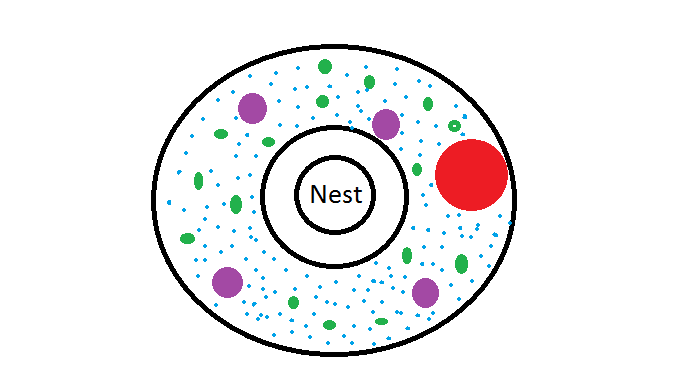
\includegraphics[width=\textwidth]{DonutShape.png}
	\caption{Distribution of Seeds in the field experiment for power law distribution with power rank 5. Red Pile indicates one large pile of 256 seeds. 4 purple piles represent 4 large piles of 64 seeds, Green color represents 16 piles of 16 seeds and blue seeds are 256 random seeds}
\end{figure}
\section{\label{section:CPFA}CPFA}
After the distribution of foods across the nest we observe their collection of seeds. It is observed that ants need longer time to discover the large pile with 256 seeds then the piles with small amount of seeds. But once the seeds are discovered, they started recruiting from the piles. Studies showed that information is transferred among the ants for larger piles with more seeds. We have plotted the collection of seeds from the field experiments and discovered ants walk randomly to collect seeds. Once they get the seed they bring it back to the nest. But if they discover a large food source they share the information with others to recruit from the food source. Once the information is shared more ants come into recruitments and while collecting this food they also share information with other ants. As soon as ants start recruiting from the food source, their foraging rate goes up. But the food source starts losing the number of seeds. As the number of seeds starts decreasing from the food source the recruitment of amount of ants also starts decreasing. Based on this behavior, an algorithm was proposed to simulate the behavior of ants. It is called Central Place Foraging Algorithm(CPFA). CPFA is an agent-based model where agents are programmed to follow ant’s strategy to collect seeds. In CPFA Ants follows three methods to collect seeds.
\begin{itemize}
	\item \textbf{Random Walk:} Ants starts walking randomly from the nest. If they find any food they bring it back to nest
	\item \textbf{Use of Internal Memory:} They remember the last position where the food was found and can return to that place for further search of food. This is method is called site fidelity.
	\item \textbf{Use of Pheromone:} They lay a pheromone trail from the food source to the nest so that other ants can follow that trail to collect food from that source.	
\end{itemize} 
Initially, a search location is selected for each of the ants. Then ants start traveling to the search site. After reaching the search site, they perform either uninformed random walk to a random location or informed random walk to a known location based on site fidelity or pheromone. If no resource is found, then they return to the nest. If they find any resource they start to sense the local resource density. Based on the local resource density they decide whether to use site fidelity in future or to lay pheromone. After sensing the resource density, the return to the nest with the seed. 
While foraging whether the agents will use any of three strategies is governed by seven parameters. These are seven parameters for CPFA
\begin{table}[h]
	\begin{tabular}{ |p{0.6\textwidth}|p{0.33\textwidth}| } 
		\hline
		\textbf{Parameters} & \textbf{Initialization Functions} \\
		\hline 
		Probability of Switching to Searching & U(0,1)\\ 
		\hline
		Probability of Returning to Nest & U(0,1)\\ 
		\hline
		Uniform Search Variation & (0, 4 PI)\\
		\hline
		Rate of Informed Searched Decay & E(20,0)\\
		\hline
		Rate of Site Fidelity & E(20,0)\\
		\hline
		Rate of Laying Pheromone & E(20,0)\\
		\hline
		Rate of Pheromone Decay & E(20,0)\\
		\hline
	\end{tabular}
	\caption{Seven parameters and their initialization, that characterizes Central Place Foraging Algorithm}
\end{table}
Parameters that are following a uniform distribution, higher the value of the parameter higher the probability of that event. For example, "probability of switching to searching" follows a uniform distribution. Higher the value of this parameter, higher the probability that the ant will switch to search. For the exponential distribution, higher the value of the parameter, lower the chance of using that feature. For example, if "Rate of Laying Pheromone" is zero, then it means that there is a higher chance of laying the pheromone. On the other hand,  a value close to 20 means that chance of using the pheromone is very low. 
The Probability of switching to searching determines the chance of ants to switch to search for resources. When ants were not primed by site fidelity or pheromone information, they select a random location to visit. And search for resources in the pre-determined location. If they can’t find any food, they select another new location. The higher the value of switching to the searching parameter, the more they search. 
The Probability of returning to nest defines the chances of returning to nest for unsuccessful foraging trip. Ants determine the position of a search location by either using site fidelity, or pheromone or randomly. When the travel to a particular location they look for resources. If they can't find any resource, they select a new location to explore and travels to that place. They keep selecting a new place to explore for a certain period of time. The parameter "probability of returning to nest comes into play in this scenario. This parameter actually decides how long the ant will keep searching new places before returning to the nest. Higher the value of the parameter, higher the ant will explore the places for resources. 
The Rate of site fidelity comes into play when the ants use site fidelity to go to an informed location where the food already exists. Lower the value of this parameter, higher the chances of following the site fidelity. The Rate of laying pheromone is the probability of laying pheromone while returning to nest from a source location. This depends on sensing of local resource density. When the ants collect seeds from a location, they sense the density of resources in nearby areas. Lower the value of “probability of laying pheromone”, higher the chances of laying pheromone. The Probability of pheromone decay determines how fast the pheromone will evaporate. When the value of the parameter is low pheromone stays in the ground for longer time. And act as vice versa.
\section{\label{section:Genetic Algorithm}Genetic Algorithm}
Genetic Algorithms are metaheuristic search algorithm inspired from natural selection and evolutionary genetics. As such they represent intelligent exploitation of a random search used to solve optimization problems. The basic techniques of GA’s are designed to simulate processes in natural systems necessary for evolution. The evolution usually starts from a population of randomly generated individuals strings that are analogous to the chromosome that we see in our DNA, and is an iterative process, with the population in each iteration called a generation. GAs simulate the survival of the fittest among individuals over the consecutive generation for solving a problem. Each individual represents a point in a search space and a possible solution. The individuals in the population are then made to go through a process of evolution. GA proceeds through the solution domain by evaluating the fitness function. 
The whole process of evolution is divided into three major section- Selection, Crossover \& Mutation.
\subsection{Selection}{\label{section:Selection} 
In selection, the individuals with better fitness are selected. Fitness function or objective function is the way to evaluate how close the genome is, to a better solution. Once individuals are selected with better fitness, crossover and mutation is applied over them.
\subsection{Crossover}{\label{section:Crossover}
A crossover site along the bit strings is randomly chosen. The values of the two strings are exchanged up to this point. The two new offspring created from this crossover are put into the next generation of the population. 
\subsection{Mutation}{\label{section:Mutation}
With some low probability, a portion of the new individuals will have some of their bits flipped. Its purpose is to maintain diversity within the population and inhibit premature convergence. Mutation alone induces a random walk through the search space. Mutation and selection create a parallel, noise-tolerant, hill-climbing algorithms.
The process is followed until a common termination condition is reached. This termination condition can be either
\begin{itemize}
	\item A solution which fulfills minimum criteria
	\item Evolution reaching a desired number of generation
	\item Reaching Maximum Fitness
	\item Reaching the maximum computation time
	\item Convergence of the solution Or 
	\item A combination of any of this.
\end{itemize}
In Short, the GA Algorithm can be defined as bellow\\
\begin{algorithm}[H]
	\begin{algorithmic}[1]
	\State Initialize the population randomly
	\State Determine the fitness of the first generation
	 \While{Desired solution is obtaind}
	 		\State Select elite population with the best fitness
	 		\State Create a new population by crossover and mutation among the elite population
	 		\State Evaluate fitness of the population
		\caption{Genetic Algorithm at a glance.}
		\EndWhile
	\end{algorithmic}
\end{algorithm}
Although GA is very effective in finding the solution in a large special domain, it has some drawbacks. If the length of the chromosome increases, the solution space may increase exponentially, which may increase the time to reach the solution domain. Also, GA mutation and crossover in an undesired region can produce useless genomes which can push the solution to some local maxima. Besides evaluating repeated genome in the same generation can increase the evaluation time. GA’s also can’t solve efficiently where the fitness function measure is a Boolean value. Evolving the GA fitness function in first come-first serve manner can increase the bottleneck of the problem.

\chapter{Method}
\begin{figure}[h]
	\includegraphics[width=\textwidth]{Method.png}
	\caption{Steps of Change Point Analysis}
\end{figure}
\section{\label{section:Setting Simulation Environment}Setting Simulation Environment}
We setup the simulation environment to mimic the field experiments. So we distributed the resources as shown in figure $3.2$ . We had three different setups for three different species of ants. The number of agents were 12, 48 and 96. The total duration of each experiment was $90$ minutes (We collected data from field experiments for $90$ minutes only). The total arena size was $20\times20$ meter. We kept the arena into this size and bounded the agents to search in this arena.  The setup is varied for \textit{Maricopa} and \textit{Desertorum}. Table $3.1$ represents the environmental setup of simulations for \textit{P. rugosus}, \textit{P. maricopa} and \textit{P. desertorum}.
\begin{table}[h]
	\begin{tabular}{ |p{0.3\textwidth}|p{0.3\textwidth}|p{0.3\textwidth}| } 
		\hline
		\textbf{Species} & \textbf{Number of Seeds} & \textbf{Radius of Seed Distribution} \\
		\hline 
		\textit{P. rugosus} & 1024 & 5-10 meter\\ 
		\hline
		\textit{P. maricopa} & 128 & 1-3 meter\\ 
		\hline
		 \textit{P. desertorum} & 128 & 1-3 meter\\
		\hline
	\end{tabular}
	\caption{Environmental Setup of simulation for three species}
\end{table}
\begin{figure}[!h]
	\frame{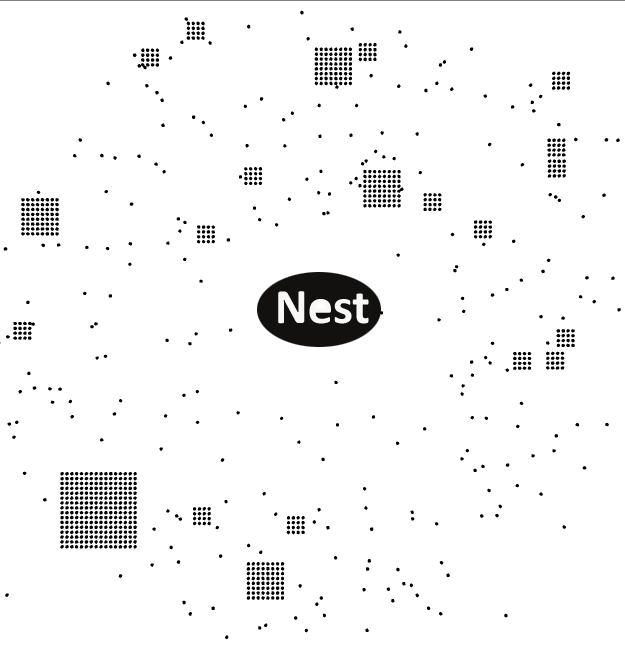
\includegraphics[scale=0.68]{ArGOS.jpg}}
	\caption{Example setup of a simulation environment for \textit{P. rugosus} with 1024 seeds three different types of piles. One large pile of $256$ seeds, four piles of $64$ seeds and sixteen piles of $16$ seeds. $256$ random seeds, are distributed uniformly inside the ring. }
\end{figure}
\section{\label{section:Tuning Parameters using Genetic Algorithm}Tuning Parameters using Genetic Algorithm}
   To analyze the data, we have tuned the parameters of CPFA. As stated above in the background study, enormous amount of parameters for CPFA can be used to evaluate the fitness. We have used the genetic algorithm to achieve the optimum set of parameters. We have divided the simulations into three categories to tune the GA for three different environments. 
   \begin{enumerate}
   	\item \textbf{Pheromone Only Parameters:}  For this type we have eliminated the use of site fidelity. Which means that the probability of using site fidelity is $20$, and remaining parameters are evolved using the GA. 
   	\item \textbf{Site fidelity Only Parameters:} In this type of experiment we eliminated the use of pheromone. For this case ants can only use site fidelity and random walk to collect resources
   	\item \textbf{Using Both site fidelity and pheromone:} This environment represents the actual field experiment condition in which agents use both site fidelity and pheromone along with the random walk.    	
   \end{enumerate}
For each type of environment, we have tuned the parameters to obtain maximum fitness using genetic algorithm where fitness is defined as maximizing the number of seeds collected in 90 minutes. Initially, we have created a population of one hundred colonies in the simulated environment. Each swarm\textquotesingle s foraging strategy is randomly initialized using the parameter setting mentioned in table $2.1$. The best genome is selected for crossover and mutation for next generation. We continued this process until we obtain the best fitness genome or parameter set. The GA is terminated either when the parameters are converged, or it reaches to generation $50$.\par  
For each swarm in a population, fitness is tested for four different random seeds. The value of random seed controls the variables of a simulation. After evaluation of each random seed for one parameter set, we have calculated the average seed collection to define the fitness of that particular swarm. These random seeds are basically numbers which are fixed for each generation. For each generation, we have selected four different numbers for the random seeds and then evaluated all the parameters for those values.\par  
To calculate the fitness for each parameter set it takes evaluating the fitness function for four times due to four different random seeds, which means for each generation it needs evaluating the objective function for $400$ times. So over $50$ generations, it will need $2000$ evaluations of the objective function. This can take a lot of time if we perform the evaluation sequentially.\par 
To remove this bottleneck, we have used multi-threading of genetic algorithm by evaluating multiple objective functions simultaneously. We have used GA Lib genetic algorithm package. The software for this work used the GAlib genetic algorithm package, written by Matthew Wall at the Massachusetts Institute of Technology. The MPI version was written by Andrew Rasmussen \url{https://github.com/andyras/GAlib-mpi/blob/master/LICENSE} who modified the code from \url{https://github.com/B0RJA/GAlib-mpi}.
The evolver.cpp file is used to initialize the GA parameters and pipe the parameters to the GA Lib.
Detail of initial parameter settings of genetic algorithm for three different setup is given in table $3.2$.
\begin{table}[h]
	\begin{tabular}{ |p{0.22\textwidth}|p{0.22\textwidth}|p{0.22\textwidth}|p{0.22\textwidth}| } 
		\hline
		\textbf{CPFA Parameters} & \textbf{Pheromone Only} & \textbf{Sitefidelity Only} & \textbf{All Parameters} \\
		\hline 
		Probability of Switching to Searching & U(0,1) & U(0,1) & U(0,1)\\ 
		\hline
		Probability of Returning to Nest & U(0,1) & U(0,1) & U(0,1)\\ 
		\hline
		Uniform Search Variation & (0, 4 PI) & (0, 4 PI) & (0, 4 PI)\\
		\hline
		Rate of Informed Searched Decay & E(20,0) & E(20,0) & E(20,0)\\
		\hline
		Rate of Site Fidelity & \textbf{E(20,20}) & E(20,0) & E(20,0)\\
		\hline
		Rate of Laying Pheromone & E(20,0) & \textbf{E(20,20}) & E(20,0)\\
		\hline
		Rate of Pheromone Decay & E(20,0) & \textbf{E(20,20}) & E(20,0)\\
		\hline
	\end{tabular}
	\caption{Initialization of seven parameters of CPFA for three different environments}
\end{table}
\section{\label{section:Generating Data Set for Analysis}Generating Data Set for Analysis}
 Once the parameters are tuned for three different environments, we have generated the data for our analysis using these parameter sets. For each of the experiment, we have extracted drop off time for each seed, location of each seed in the arena. Drop time is when it is dropped off at the nest. We have tagged each ant with distinct ID. For each seed, we also have extracted which ant has collected that seed. Also, we have tracked when the pheromone is laid, and followed, and when the site fidelity is followed. We have assigned distinct ID number to each pile so that when a pheromone trail is laid we can track which pile the trail is coming from.\par
 For each type of environment, we have simulated $500$ experiments and generated data mentioned above. We varied the value of random seed for each experiment while keeping the CPFA parameters constant for a particular environment. We also varied the position of seeds for each experiment. Each experiment was performed for $90$ minutes.\par 
 While generating the data for ``pheromone only parameters'', we did not extract any site fidelity data, because we tuned all the parameters not to use site fidelity data. Similarly, for ``site fidelity only'' experiments we did not extract any pheromone data as there was no pheromone. We have collected both site fidelity data and pheromone data when we have used both methods together for collecting resources.
 \section{\label{Analyzing The Foraging Data}Analyzing The Foraging Data}
 After generating all the data from the simulation, we have tried to observe how the ants collect seeds from different food distributions. We have observed that it takes some time for them to discover the larger piles. Once they discover it, they start to collect seeds from those piles. They use site fidelity and pheromone for this recruitment. Once they start collecting this seeds we see an increase in their foraging rate. So, we tried to detect those changes in their foraging rate by applying the change point detection algorithm. 
 \subsection{\label{Creating Timeline for each type of distribution}Creating Timeline for each type of distribution}
 We have studied each experiment separately to analyze the change in their foraging rate. For each experiment, we studied foraging rate for each type of pile individually. To study foraging rate for each pile we have created a time-line for each type of distribution. We have calculated foraging rate in overlapping windows, where each window has a fixed size and slided by a fixed time (such as 10 seconds) to create overlapping windows. Figure 3.3 shows the overlapping window for time-line. \par 
 \begin{figure}[h]
 	\includegraphics[width=\textwidth]{SlidingWindow.png}
 	\caption{An example of overlapping windows of foraging rate.}
 \end{figure}
 \begin{figure}[h]
 	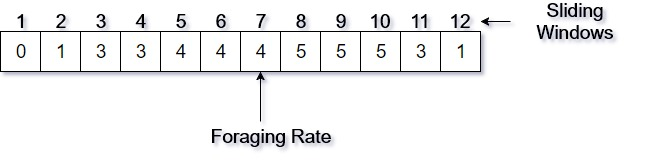
\includegraphics[width=\textwidth]{TimeLine.jpg}
 	\caption{An example of a timeline for a distribution where numbers at the top represent the sliding window number. Values in the boxes are the rate of collection of seeds per window.}
 \end{figure}
The length of the window is fixed to average time required for two round trips unless stated otherwise. For the simulated experiments it is 266 seconds. Sliding amount is fixed to 10 seconds. So if the experiment is for $90$ minutes ($5400$ seconds), we kept the length of the sliding windows for $266$ seconds and slided it by $10$ seconds, we get total $540$ sets of data where we calculated their foraging rate for a particular pile.\par 
 Once we have created the time-line for each experiment for a particular distribution of seeds we used change point detection algorithm to detect the change in the rate of collection of seeds. Another method we have created the timeline is by taking into consideration the change in the rate of foraging. In this method for creating the timeline instead of foraging rate, we take into consideration the change in foraging rate.\par
 \begin{figure}[h]
 	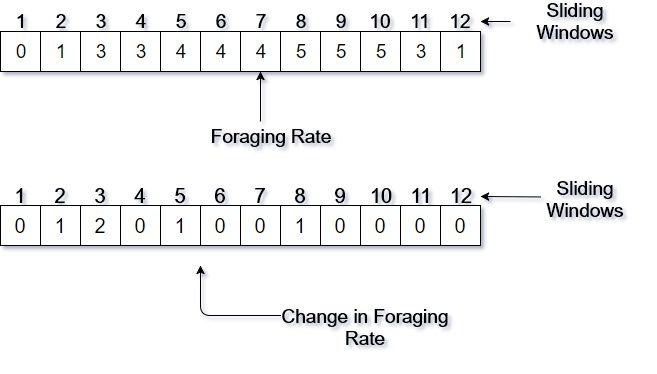
\includegraphics[width=\textwidth]{ChangeInForagingRate.jpg}
 	\caption{An example of timeline and change in foraging rate. The change in foraging rate is calculated by measuring the difference between the timeline windows}
 \end{figure}
\section{\label{section:Change Point Detection Algorithm}Change Point Detection Algorithm}
 The change point detection algorithm is divided into two parts. First part is the adding rate of collecting seeds to calculate the cumulative sum and detrend for smoothing. And the second part is applying the change point detection algorithm. We have used binary segmented cumulative sum method to determine the change points.
 \subsection{\label{Calculating the Cumulative Sum}Calculating the Cumulative Sum}
 The calculation of cumulative sum is basically adding the foraging rate in each window. Figure $3.6$ and algorithm $3.1$ demonstrates how the cumulative sum is calculated.\par
 \begin{figure}[h]
 	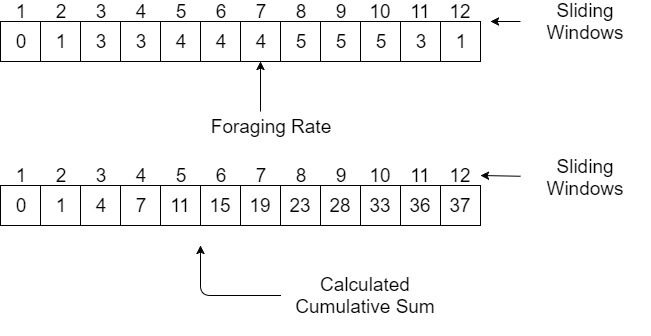
\includegraphics[width=\textwidth]{CumulativeSum.jpg}
 	\caption{This figure demonstrates how the cumulative sum is calculated from the timeline of foraging rate.}
 \end{figure}

 \begin{algorithm}[H]
 	\begin{algorithmic}[1]
 		\State Sum=0
 		\For{i=1:Number of Sliding Window} 
 			\State Sum= Sum + window(i)
 			\State CumulativeSum(i)=Sum
 		\EndFor
 		\caption{Pseudo code for calculating cumulative sum.}
 		\label{Pseudo code for calculating cumulative sum.}
 	\end{algorithmic}
 \end{algorithm}
 
 \subsection{\label{Detrending}Detrending}
 A time series trend is defined as a long-term change in the mean. The removal of a trend in a statistical or mathematical operation of time series is called detrending. It is often applied to remove features which are obsolete or unimportant. In time series analysis, detrending is also used in preprocessing step to prepare data set for further analysis.\par 
 There are several methods of detrending. Linear trends in mean can be truncated by subtracting a least-square-fit straight line. Different procedures are used for more complicated trend. For example, the cubic smoothing spline is commonly used in dendrochronology to fit and remove ring-width trend that might not be linear, or not even monotonically increasing or decreasing over time. It is important to understand the effect of detrending on spectral properties of time series before trying to remove the trend from the time series.\par 
 Before applying the change point detection algorithm, we have applied detrending algorithm to remove the trend from the time series. We used linear detrending and constant detrending to observe the effect of detrending in our time series data. Linear detrending removes the linear trend from the data where constant detrending removes the mean from the data. Figure $3.7$ demonstrates how linear and constant detrending affect the time series.\par
 \begin{figure}[H]
 	\begin{subfigure}{\textwidth}
 		\centering
 		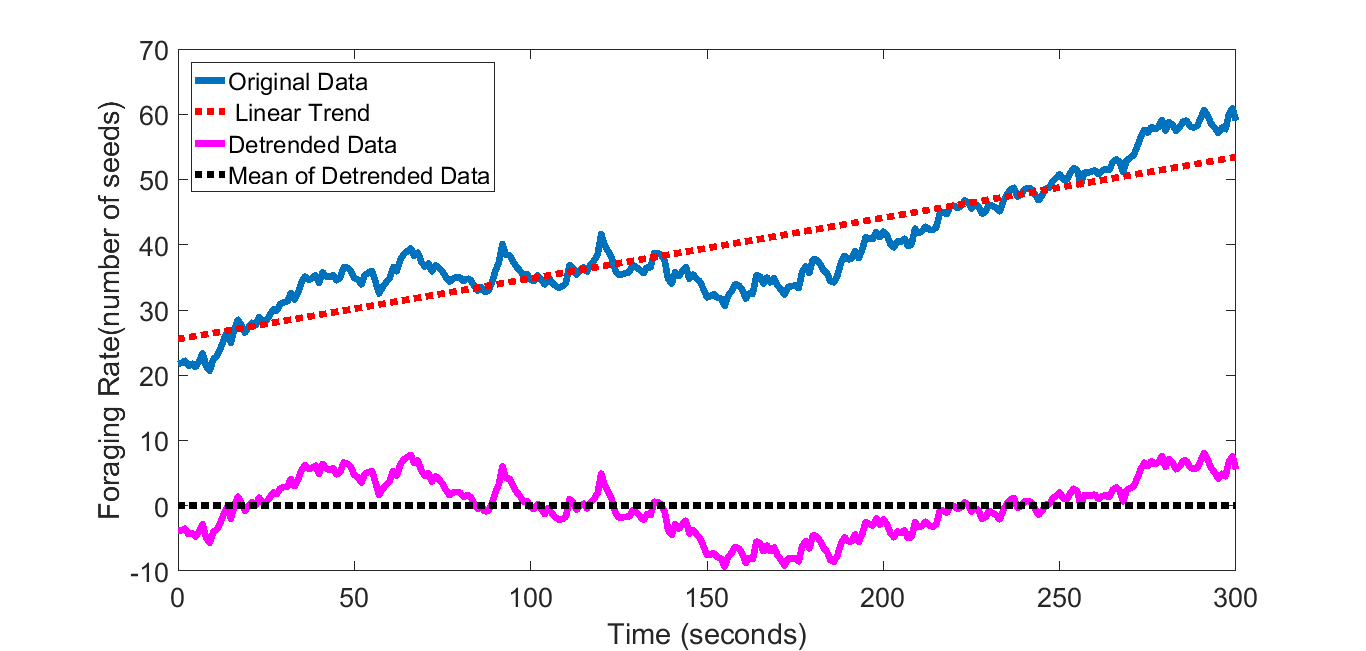
\includegraphics[width=\linewidth, height=0.3\textheight]{linearDetrending.jpg}
 		\caption{Linear Detrending}
 		\label{fig:Linear}
 	\end{subfigure}%
 	\\
 	\begin{subfigure}{\textwidth}
 		\centering
 		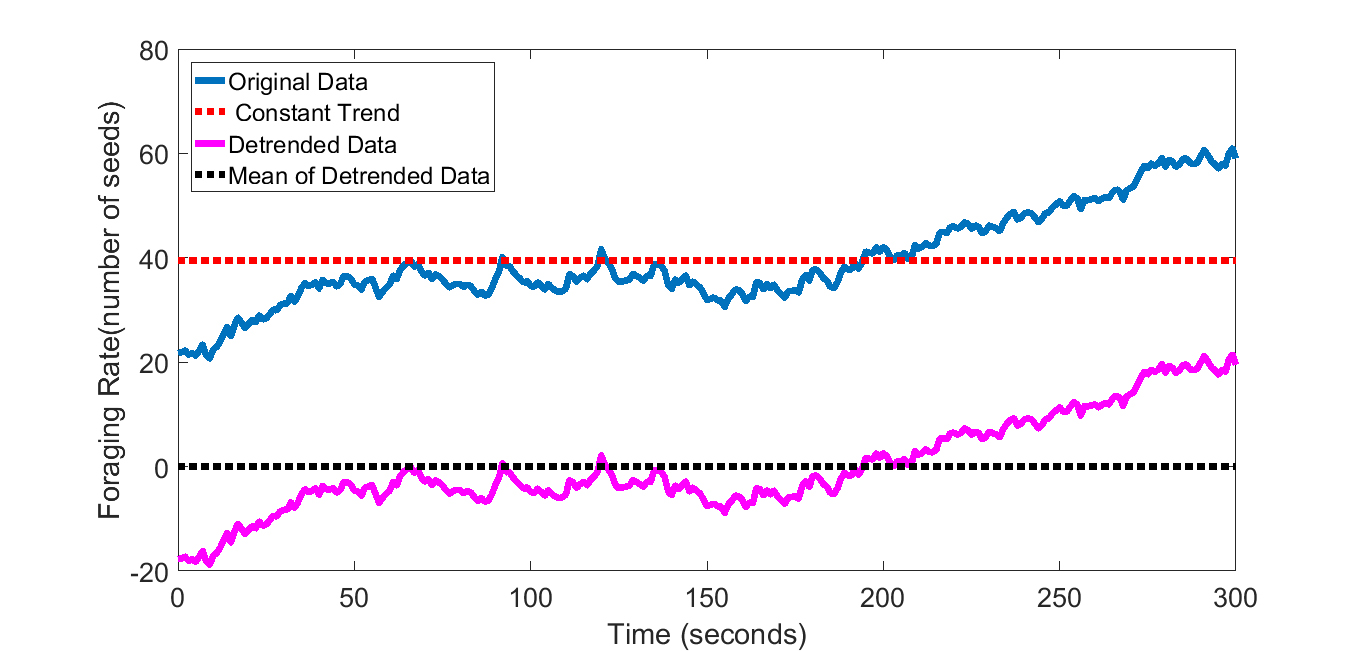
\includegraphics[width=\linewidth, height=0.3\textheight]{constantDetrending.jpg}
 		\caption{Constant Detrending}
 		\label{fig:Constant}
 	\end{subfigure}
 	\caption{An example of applying linear and constant detrending on the cumulative sum of a timeline from one simulated CPFA experiment.}
 	\label{fig:fig}
 \end{figure}
 \clearpage
\subsection{\label{Binary-Segmented Cumulative Sum}Binary-Segmented Cumulative Sum}
Binary Segmentation is one of the most established search method used for detecting the change point. This method extends any single change point method to multiple change points by iteratively repeating the method on different subsets of the sequence.\par 
To perform binary segmentation, we first apply the chosen single change point detection method to the entire data set, if no change point is found then we are done. If a change point is detected, call this $\tau$, then the data is split into two segments, timeline$[1:\tau]$ and timeline$[\tau+1:n]$. We then apply the single change point method to the two segments and repeat iteratively. We stop when no more change points are detected.\par
Binary segmentation is a very fast algorithm with complexity $O(n\log n)$ to detect the changes. But the major disadvantage of its computational speed is that it gives us only an approximation of changes. It is not guaranteed that the binary segmentation method will find us the optimum solution. Also due to iterative nature of this algorithm, it may not detect changes small changes. Thus, to verify the how well this method is performing, we have verified the results with the simulated data. 
The pseudo code for the binary segmentation algorithm is given in Algorithm $3.2$. 

\begin{algorithm}[!h]
	\begin{algorithmic}[1]
		 \State \algorithmicrequire A set of data of the form ($value_1$,$value_2$,$value_3$...)\\
		\qquad\quad\enspace A test statistic $\tau(.)$\\
		\qquad\quad\enspace An estimator of the changepoint position $\tau(.)$\\
		\qquad\quad\enspace A rejection threshold $\beta$
		\State\textbf{Initialize:} Let $C=\phi$, and $S=[1:n]$
		\While {$S\neq\phi$}
			\State Choose an element of S
			\State Denote this element as $[s,t]$
			\If{$ \tau (ys:t)<\beta $}
				\State remove$[s,t] from S$
			\EndIf
			\If {$\tau(ys:t)\geq\beta$}
				\State remove$[s,t] from S$
				\State calculate $ r=\tau(ys:t)+s-1 $, 
				\State add r to C
				\If {$r\neq s$}
					\State add $[s,r]$ to $S$
				\EndIf
				\If {$r=t-1$}
					\State $[r+1,t]$ to $S$
				\EndIf
			\EndIf
		\EndWhile	
		\caption{Pseudocode for Binary Segmented Mean Cumulative Sum}
		\label{Pseudocode for Binary Segmented Mean Cumulative Sum}
	\end{algorithmic}
\end{algorithm}
\clearpage
\section{\label{section:Verification of Change Points}Verification of Change Points}
As we have simulated data, and we know when the pheromones and site fidelities are used in simulations, we can certainly verify how efficient our change points detection algorithms are. So to check how efficient is our algorithms to detect change points, we divided the detection of change points into 4 categories.
\begin{itemize}
	\item \textbf{Catagory A or $\le 10$:} Change point detection within 10 seconds of pheromone laying events, 
	\item \textbf{Catagory B or $11-300$:} Change point detections within 11-300 seconds of pheromone laying events, 
	\item \textbf{Catagory C or $>300$:} Change point detections after more than 300 seconds of pheromone laying events and 
	\item \textbf{Catagory D or None:} Change point detected but no pheromone laying events has happened. 
\end{itemize} 
%So we have compared the results of four different methods based on this 4 categories using the data extracted from our simulation.
\clearpage
\section{\label{section:Applying the best method on Field Data}Applying the best method on Field Data}
We applied change point detection on 6 different types of the data set. This led us to evaluate the performance of change point detection algorithm for six different methods.
\begin{figure}[!ht]
	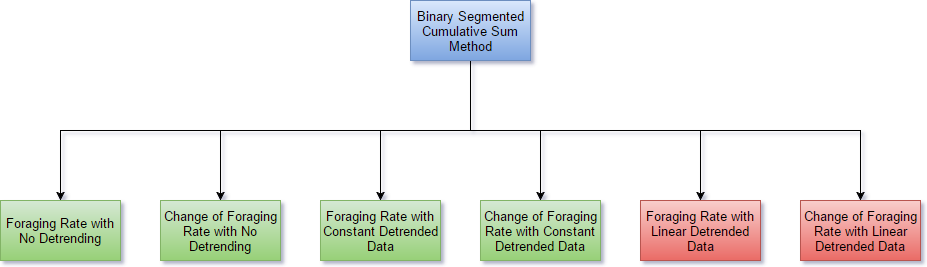
\includegraphics[width=\textwidth]{ChangePoint.png}
	\caption{Change point analysis on an alternate dataset}
\end{figure}
After validating six different methods that we have applied to simulation data. We select the best method for them based on the performance on six categories stated above, and we apply the best method in our field data.   


\chapter{Results}
\section{\label{section:overview}Overview}
   The classic approach to proving a theorem is some really difficult 
   mathematics.  For the theory of relativity, I asked grandpa Al exactly 
   how he proved it.  He gave me a few hints, including some stuff about
   rest mass and big electro-motive force.  I think he is really smart.
\section{Conclusions}
   I conclude that this is a really short thesis.
\chapter{Conclusion}
\section{\label{section:overview}Overview}
   The classic approach to proving a theorem is some really difficult 
   mathematics.  For the theory of relativity, I asked grandpa Al exactly 
   how he proved it.  He gave me a few hints, including some stuff about
   rest mass and big electro-motive force.  I think he is really smart.
\section{Conclusions}
   I conclude that this is a really short thesis.
\chapter{Appendicies}
\begin{figure}[h]
	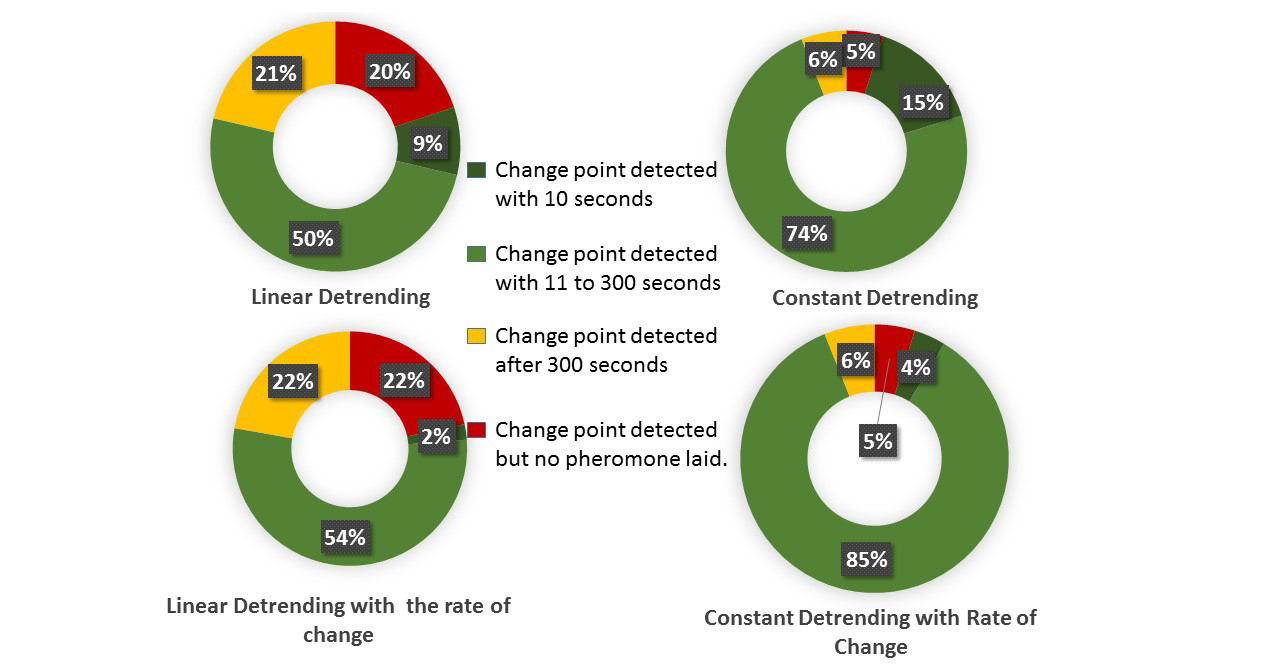
\includegraphics[height=0.35\textheight]{DonutCharts/Slide2.JPG}
	\caption{Efficiency chart for \textit{P. Rugosus}, one pile,  communication only setting.}
\end{figure}
\begin{figure}[h]
	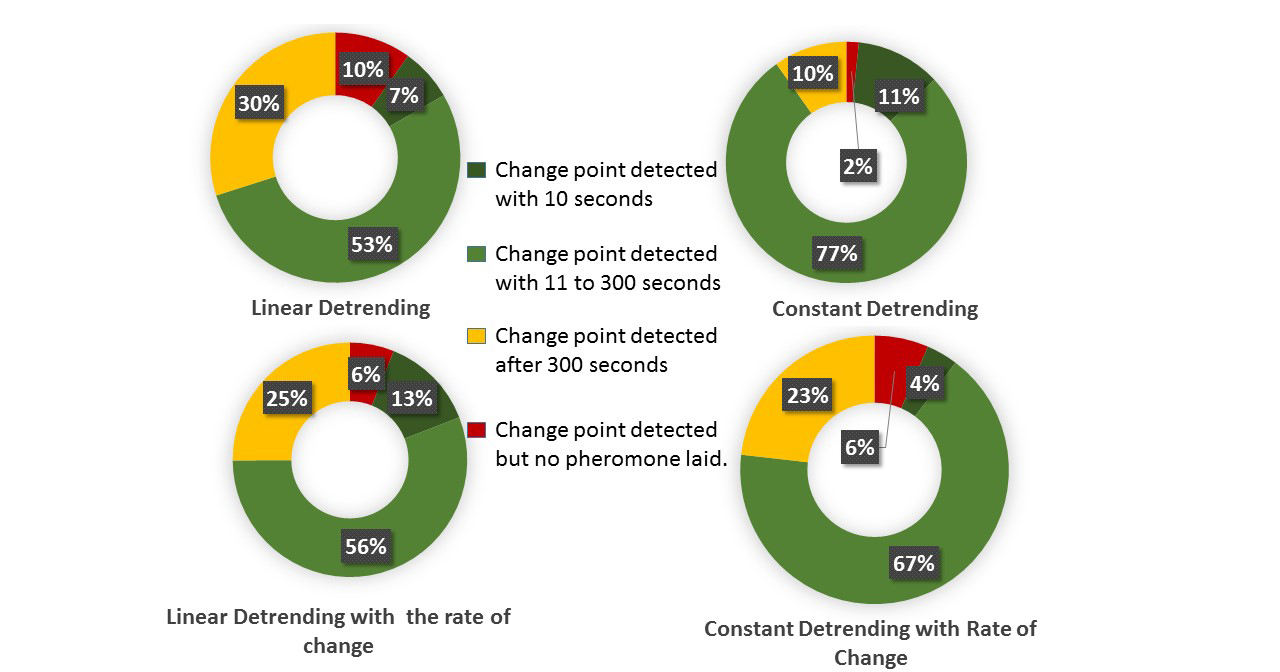
\includegraphics[height=0.35\textheight]{DonutCharts/Slide3.JPG}
\caption{Efficiency chart for \textit{P. Rugosus}, four pile,  communication only setting.}
\end{figure}
\begin{figure}[h]
	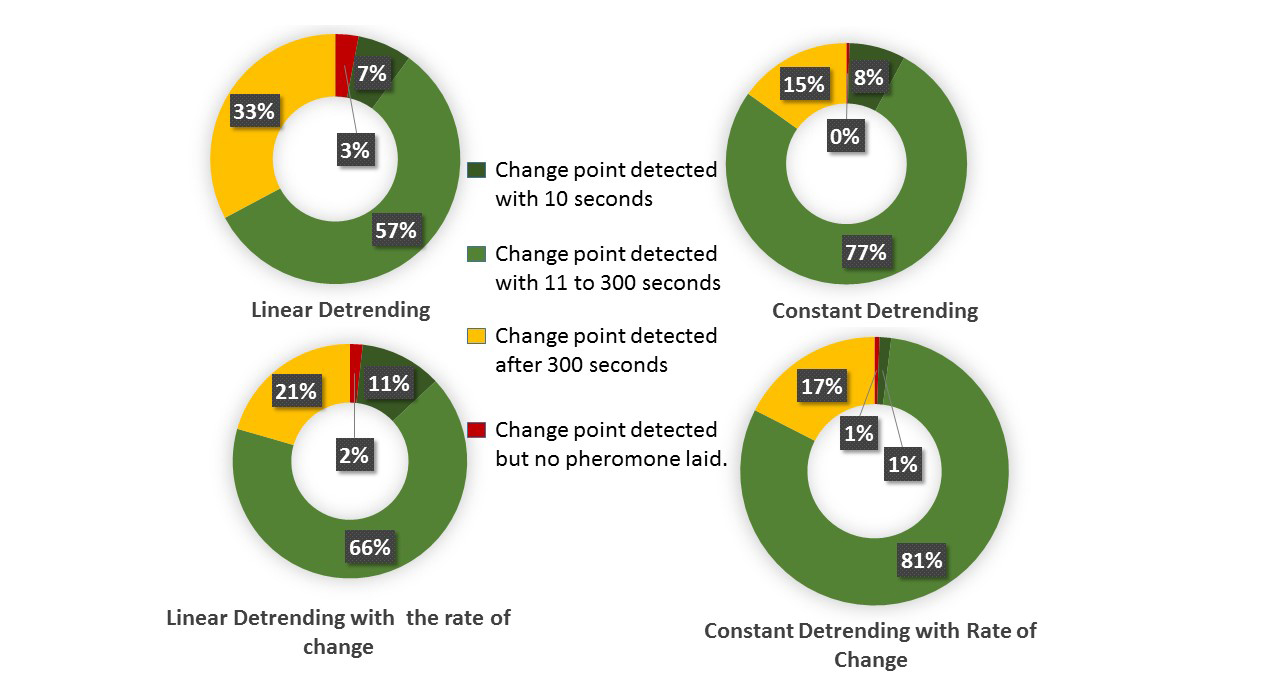
\includegraphics[height=0.35\textheight]{DonutCharts/Slide4.JPG}
	\caption{Efficiency chart for \textit{P. Rugosus}, sixteen pile,  communication only setting.}
\end{figure}
\begin{figure}[h]
	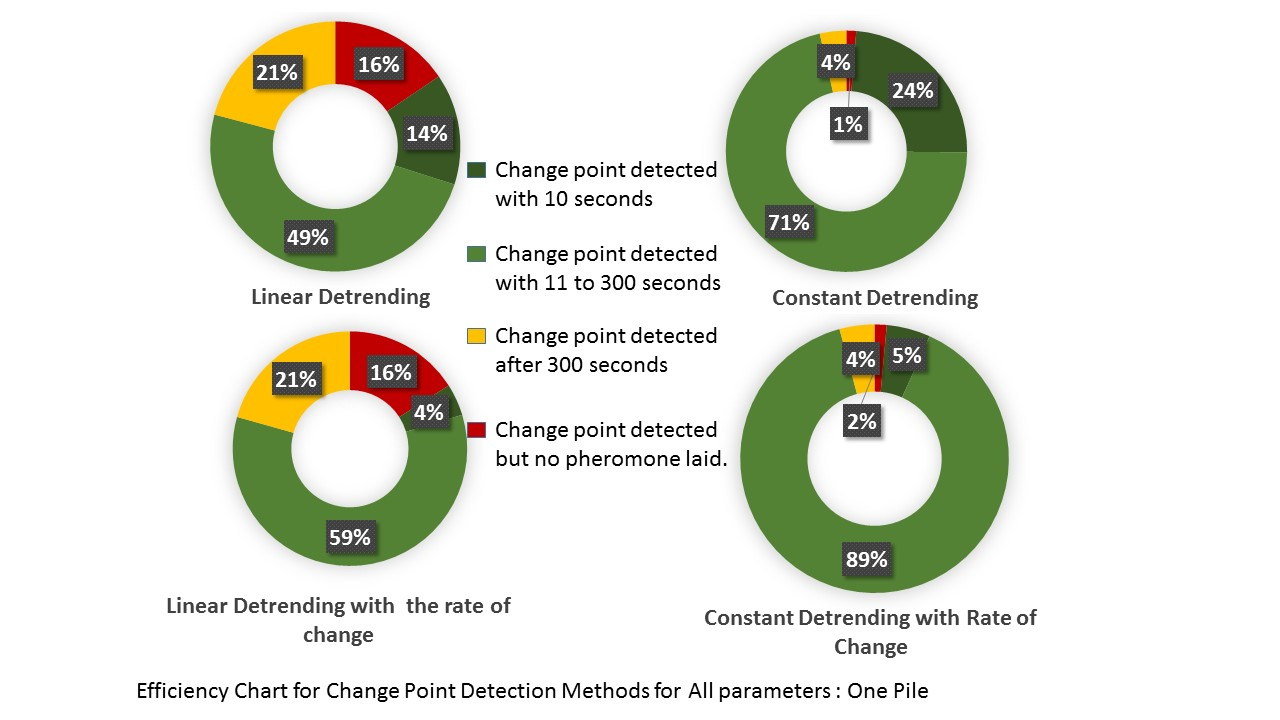
\includegraphics[height=0.35\textheight]{DonutCharts/Slide5.JPG}
	\caption{Efficiency chart for \textit{P. Rugosus}, one pile,  memory and communication combined setting.}
\end{figure}
\begin{figure}[h]
	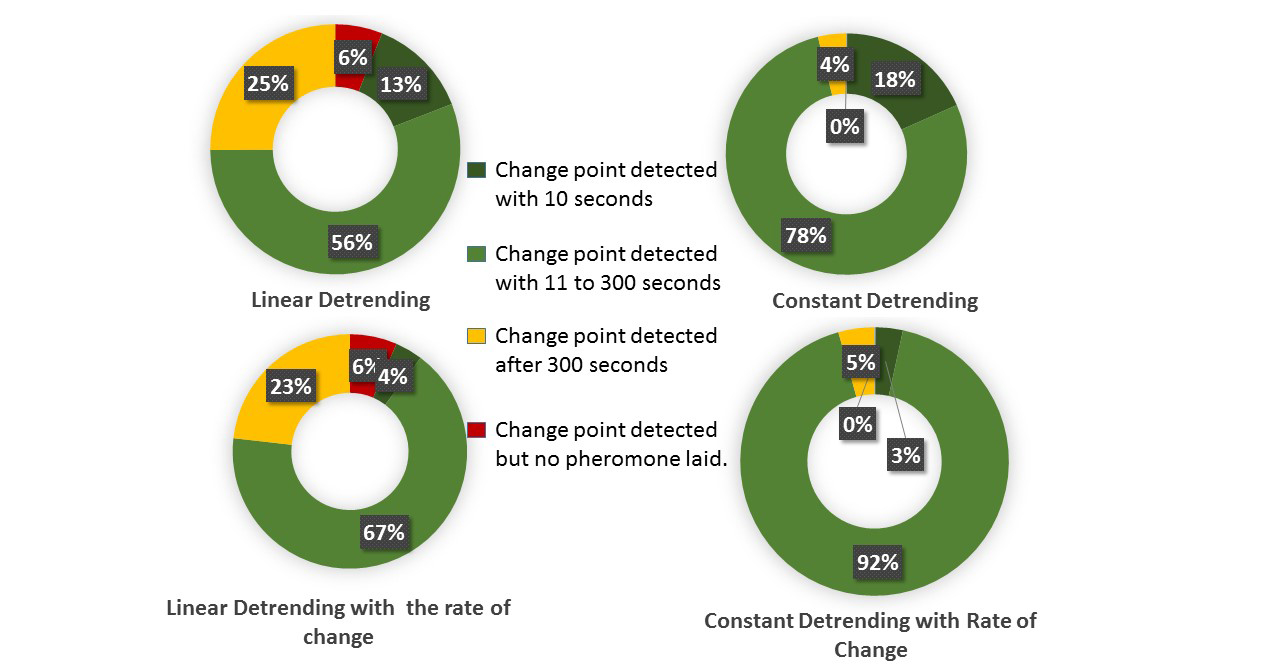
\includegraphics[height=0.35\textheight]{DonutCharts/Slide6.JPG}
	\caption{Efficiency chart for \textit{P. Rugosus}, four pile, memory and communication combined setting.}
\end{figure}
\begin{figure}[h]
	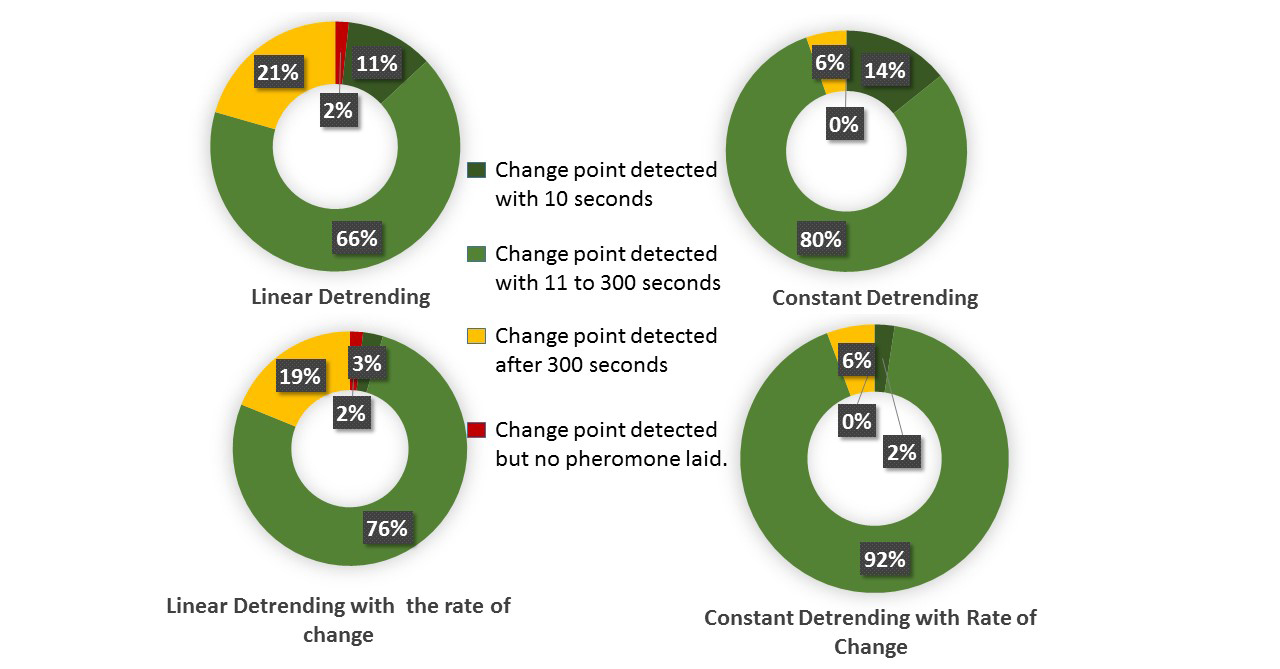
\includegraphics[height=0.35\textheight]{DonutCharts/Slide7.JPG}
	\caption{Efficiency chart for \textit{P. Rugosus}, sixteen pile,  memory and communication combined setting.}
\end{figure}
\begin{figure}[h]
	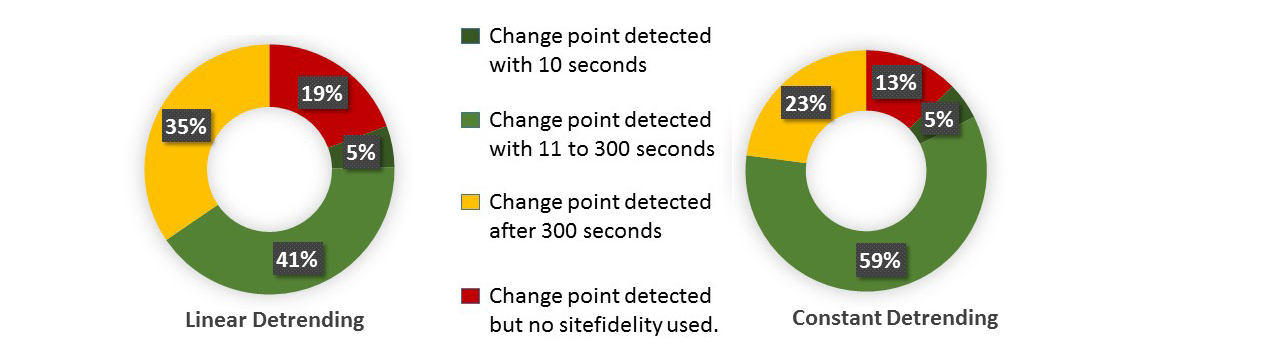
\includegraphics[width=\textwidth]{DonutCharts/Slide8.JPG}
	\caption{Efficiency chart for \textit{P. Rugosus}, one pile,  memory only setting.}
\end{figure}
\begin{figure}[h]
	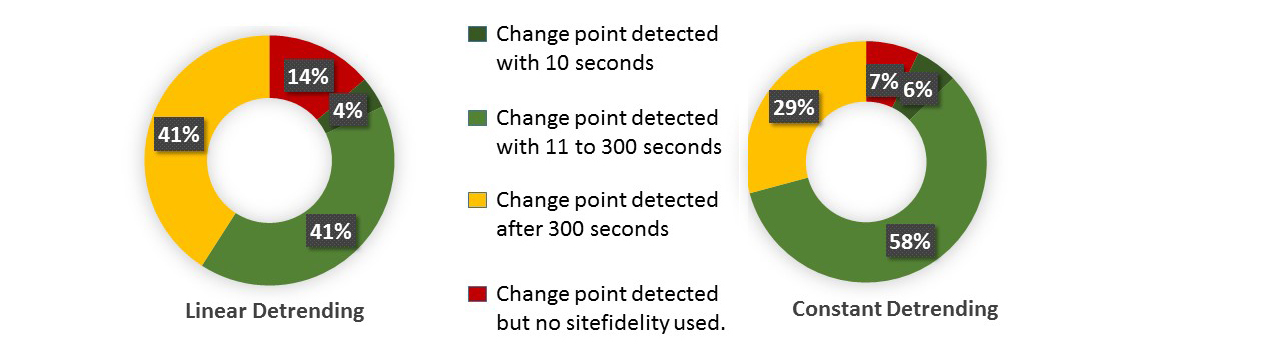
\includegraphics[width=\textwidth]{DonutCharts/Slide9.JPG}
	\caption{Efficiency chart for \textit{P. Rugosus}, four pile,  memory only setting.}
\end{figure}
\begin{figure}[h]
	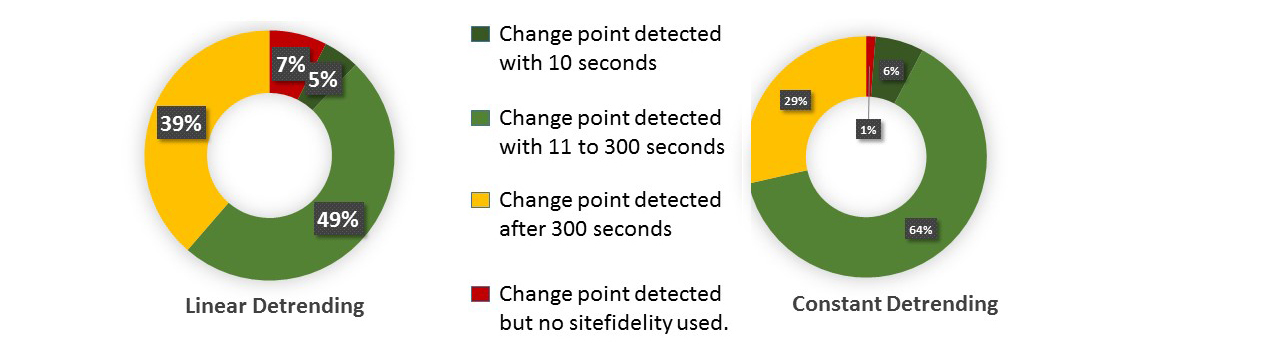
\includegraphics[width=\textwidth]{DonutCharts/Slide10.JPG}
	\caption{Efficiency chart for \textit{P. Rugosus}, sixteen pile,  memory only setting.}
\end{figure}
\begin{figure}[h]
	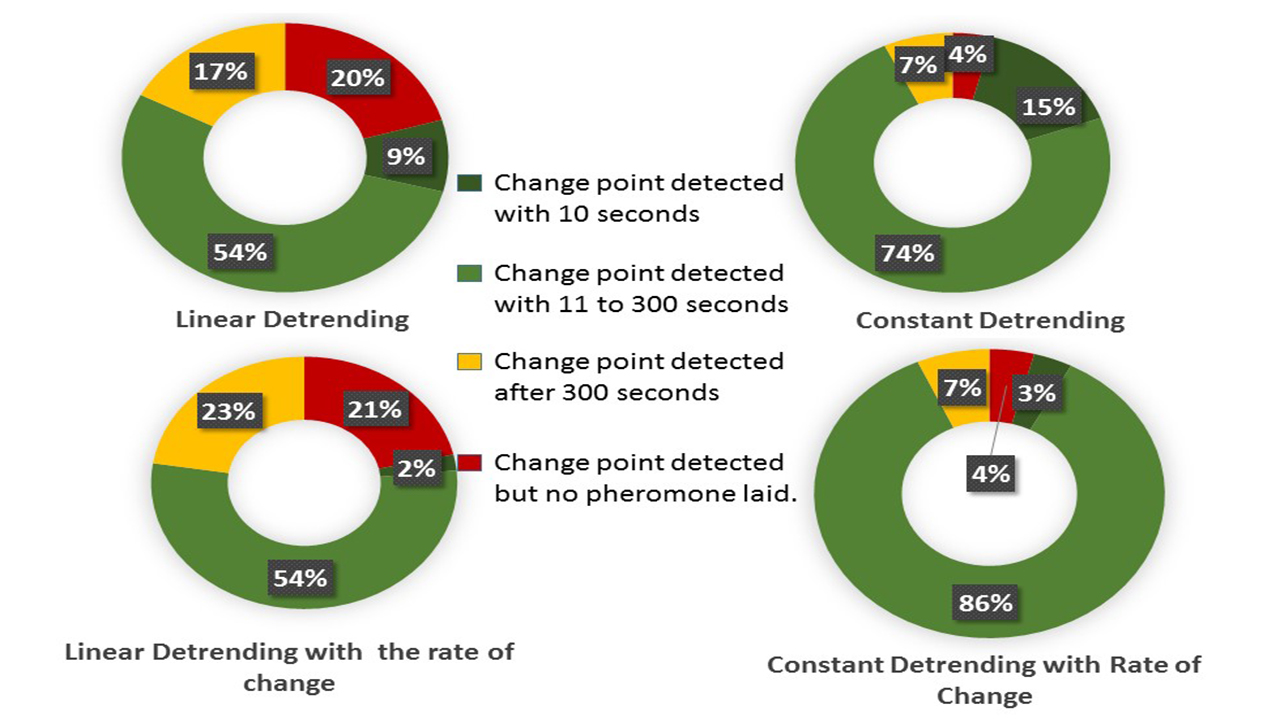
\includegraphics[height=0.35\textheight]{DesertorumDonutCharts/Slide12.JPG}
	\caption{Efficiency chart for \textit{P. Desertorum}, one pile,  communication only setting.}
\end{figure}
\begin{figure}[h]
	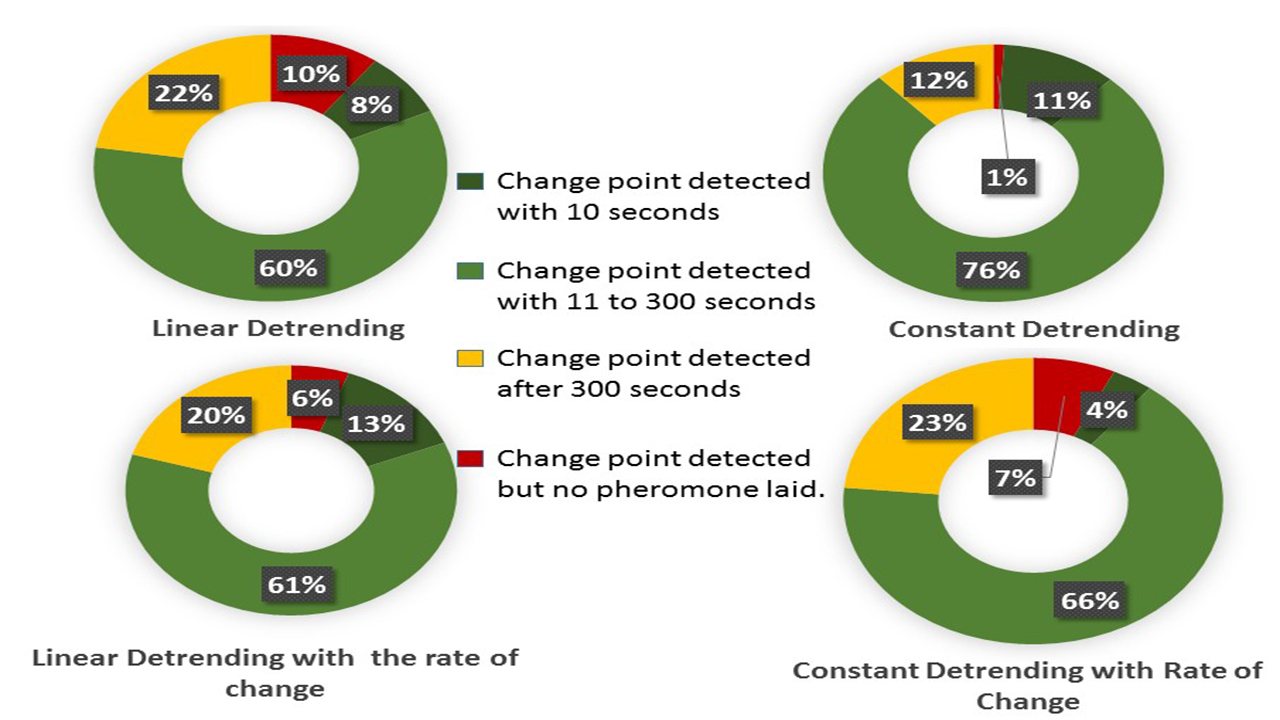
\includegraphics[height=0.35\textheight]{DesertorumDonutCharts/Slide13.JPG}
	\caption{Efficiency chart for \textit{P. Desertorum}, four pile,  communication only setting.}
\end{figure}
\begin{figure}[h]
	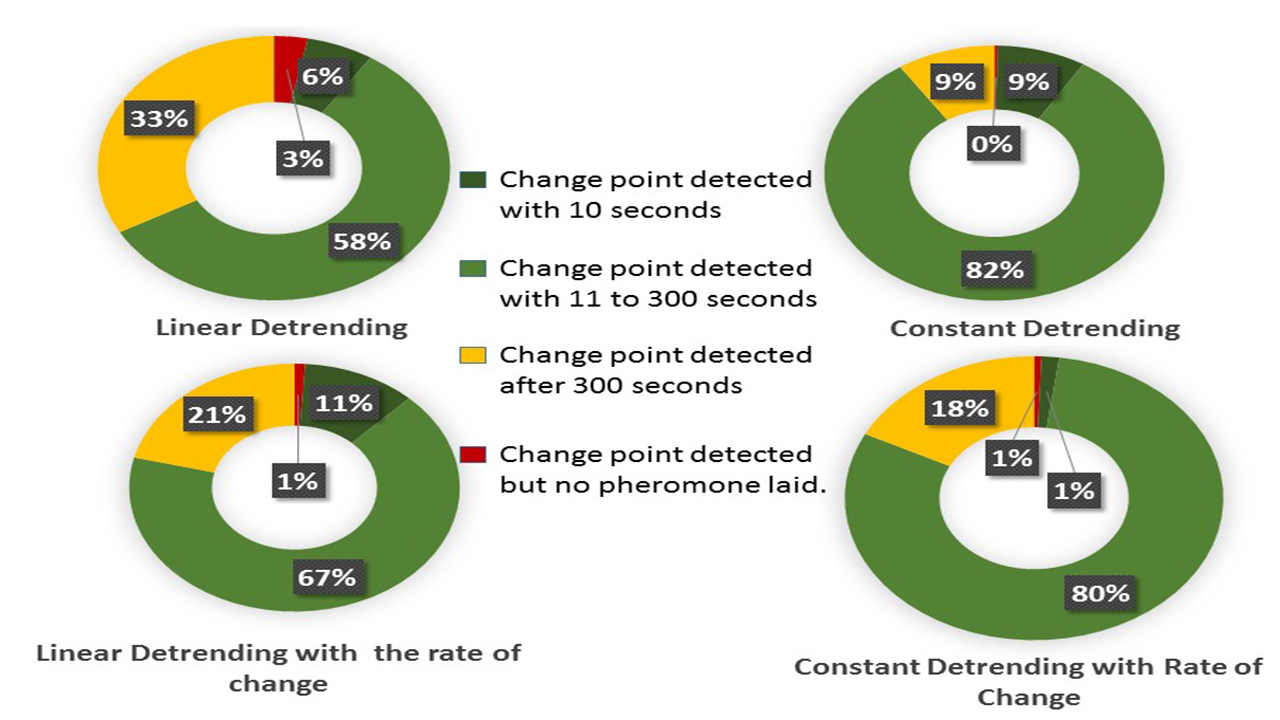
\includegraphics[height=0.35\textheight]{DesertorumDonutCharts/Slide14.JPG}
	\caption{Efficiency chart for \textit{P. Desertorum}, sixteen pile,  communication only setting.}
\end{figure}
\begin{figure}[h]
	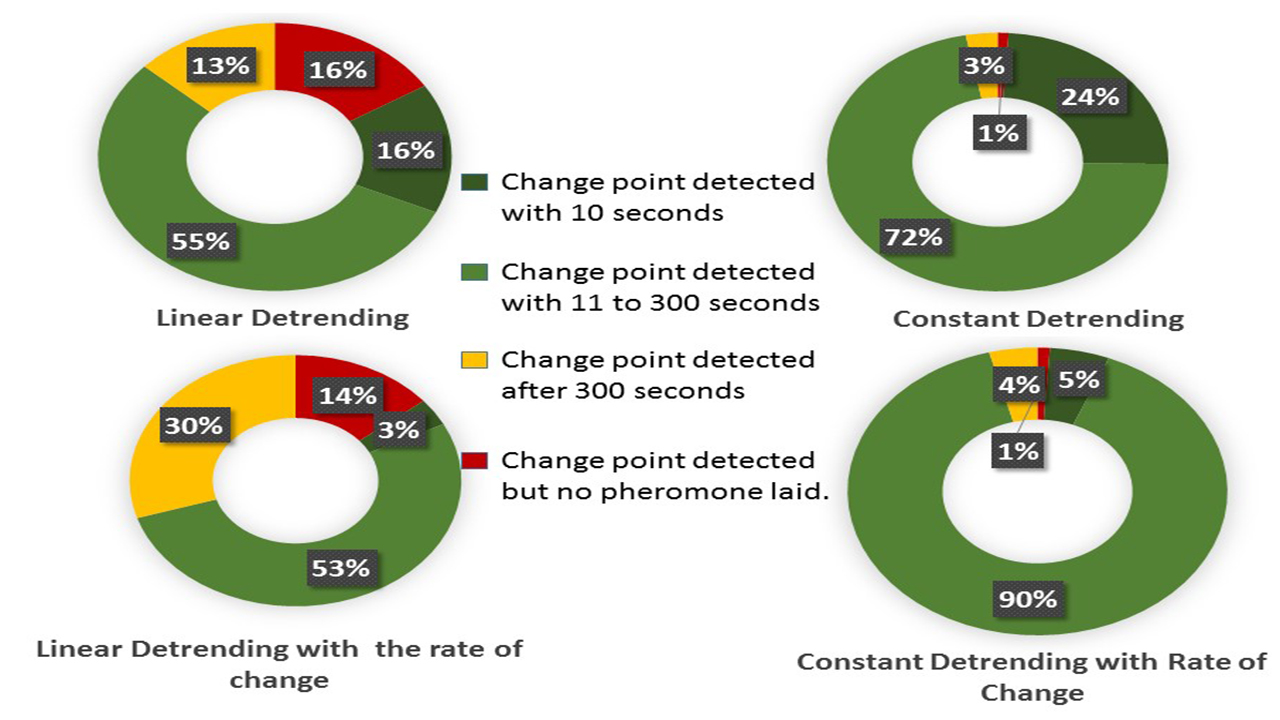
\includegraphics[height=0.35\textheight]{DesertorumDonutCharts/Slide15.JPG}
	\caption{Efficiency chart for \textit{P. Desertorum}, one pile,  memory and communication combined setting.}
\end{figure}
\begin{figure}[h]
	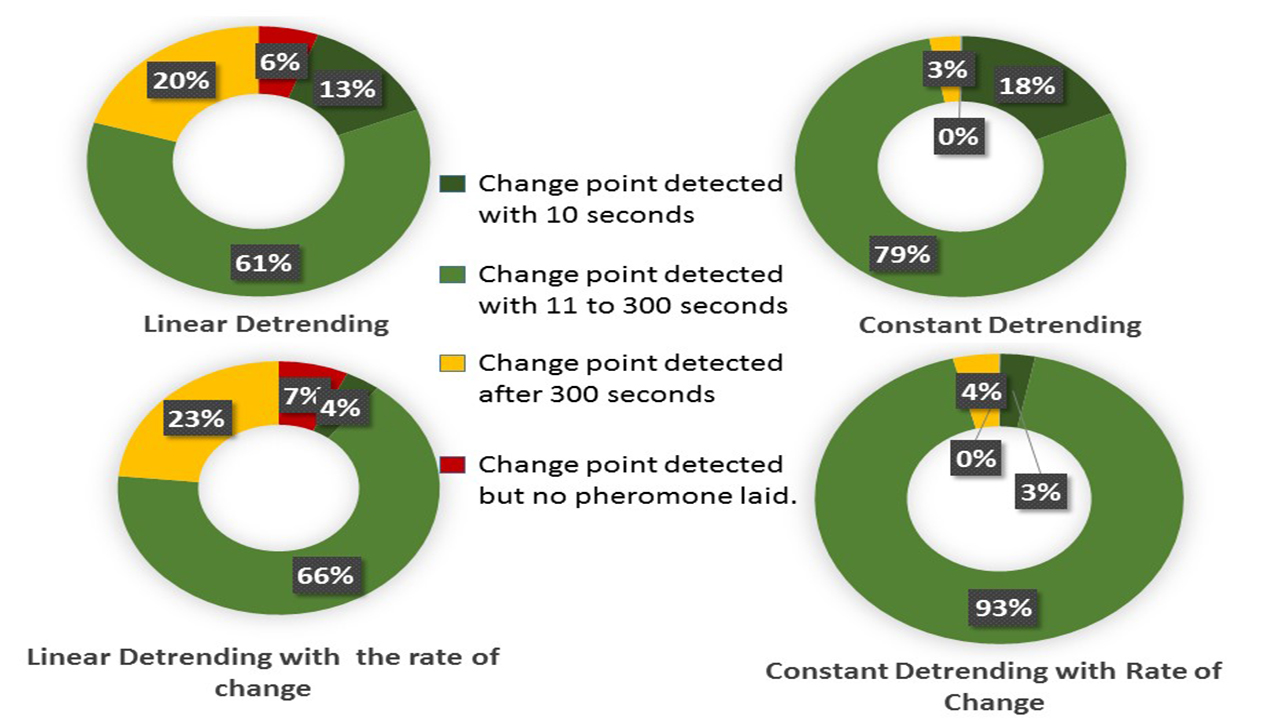
\includegraphics[height=0.35\textheight]{DesertorumDonutCharts/Slide16.JPG}
	\caption{Efficiency chart for \textit{P. Desertorum}, four pile, memory and communication combined setting.}
\end{figure}
\begin{figure}[h]
	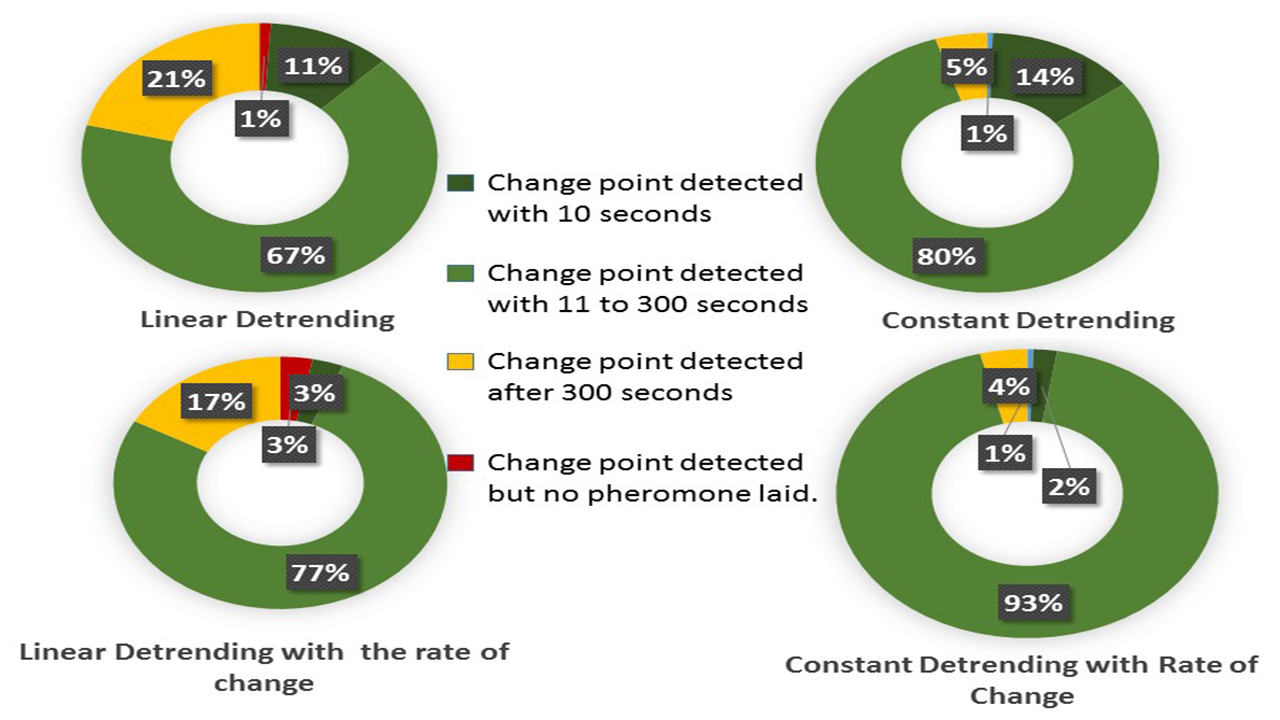
\includegraphics[height=0.35\textheight]{DesertorumDonutCharts/Slide17.JPG}
	\caption{Efficiency chart for \textit{P. Desertorum}, sixteen pile,  memory and communication combined setting.}
\end{figure}
\begin{figure}[h]
	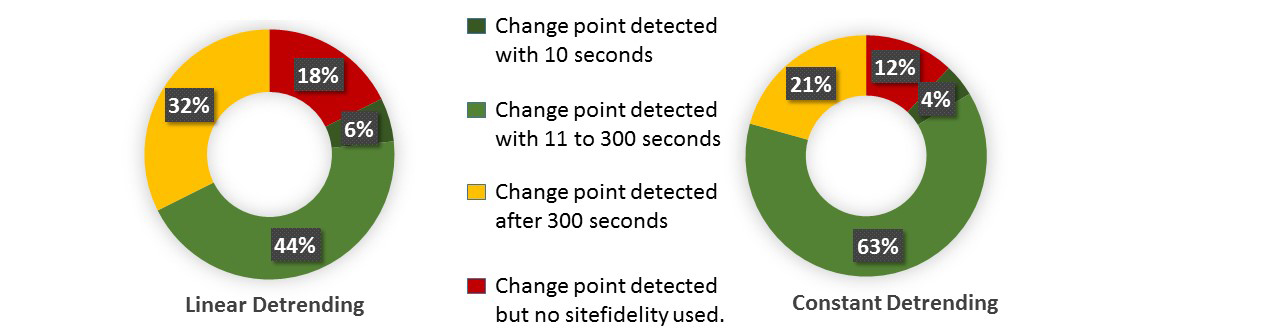
\includegraphics[width=\textwidth]{DesertorumDonutCharts/Slide18.JPG}
	\caption{Efficiency chart for \textit{P. Desertorum}, one pile,  memory only setting.}
\end{figure}
\begin{figure}[h]
	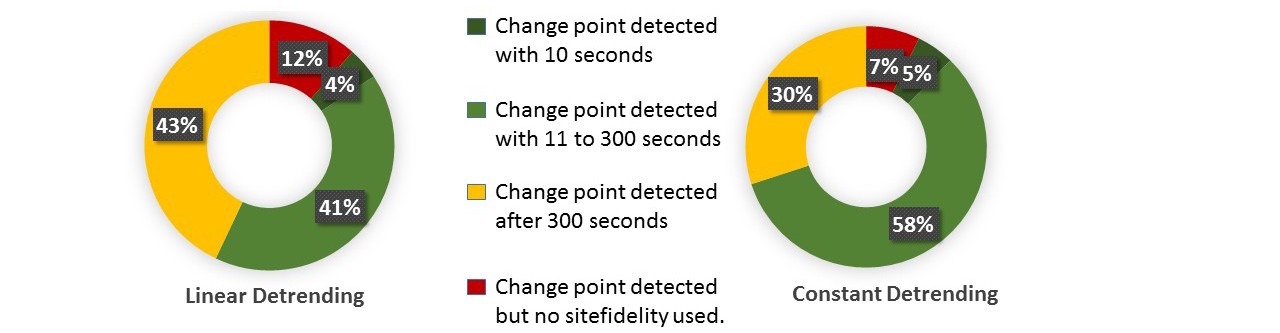
\includegraphics[width=\textwidth]{DesertorumDonutCharts/Slide19.JPG}
	\caption{Efficiency chart for \textit{P. Desertorum}, four pile,  memory only setting.}
\end{figure}
\begin{figure}[h]
	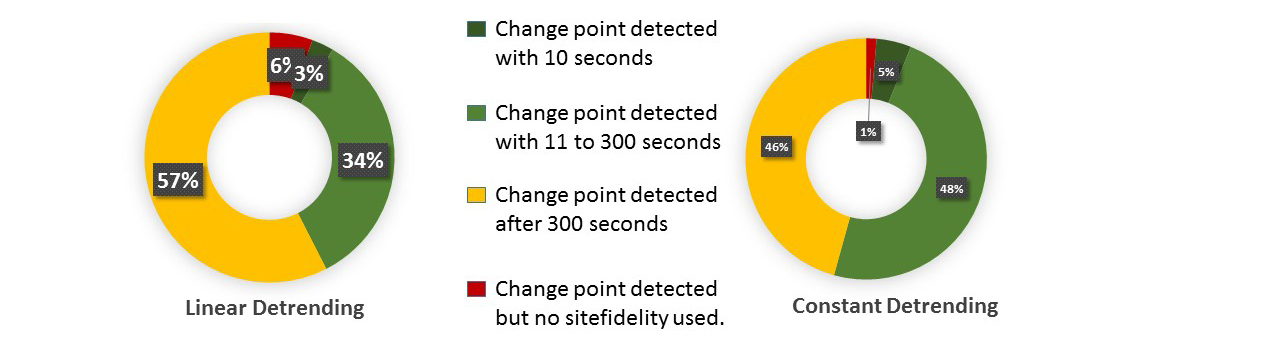
\includegraphics[width=\textwidth]{DesertorumDonutCharts/Slide20.JPG}
	\caption{Efficiency chart for \textit{P. Desertorum}, sixteen pile,  memory only setting.}
\end{figure}
\clearpage
\begin{figure}[h]
	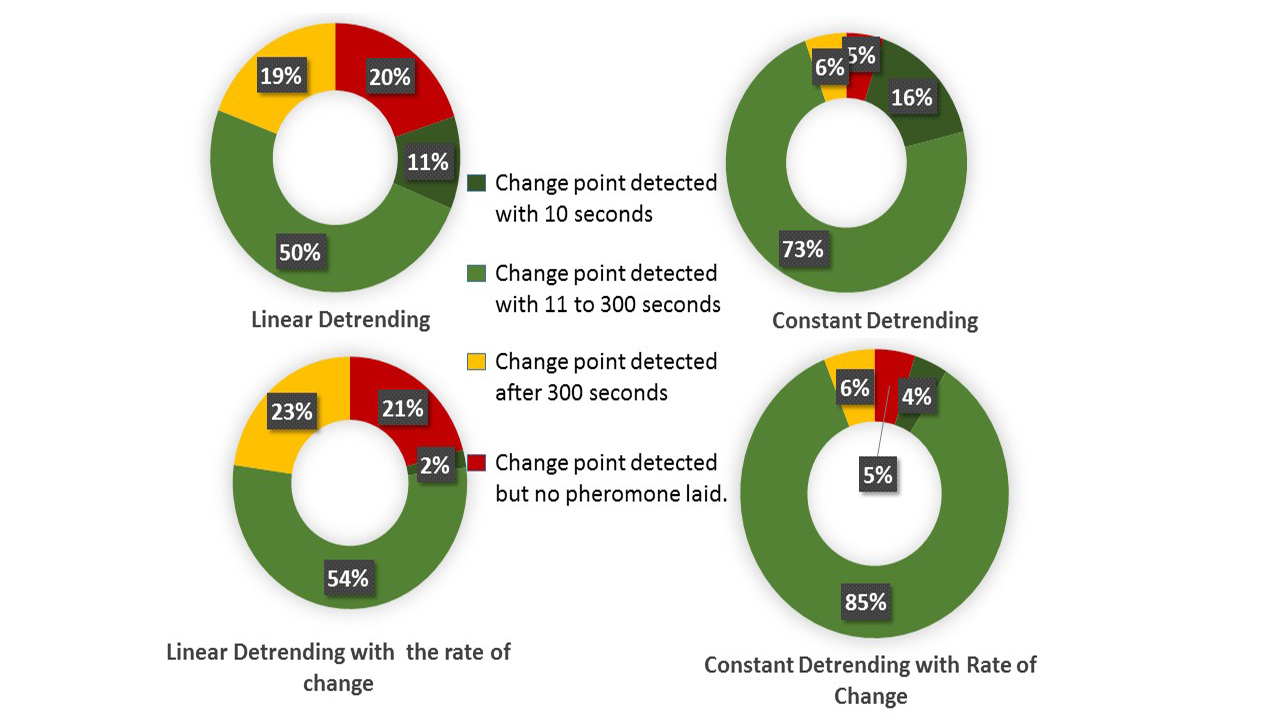
\includegraphics[height=0.35\textheight]{MaricopaDonutCharts/Slide22.JPG}
	\caption{Efficiency chart for \textit{P. Maricopa}, one pile,  communication only setting.}
\end{figure}
\begin{figure}[h]
	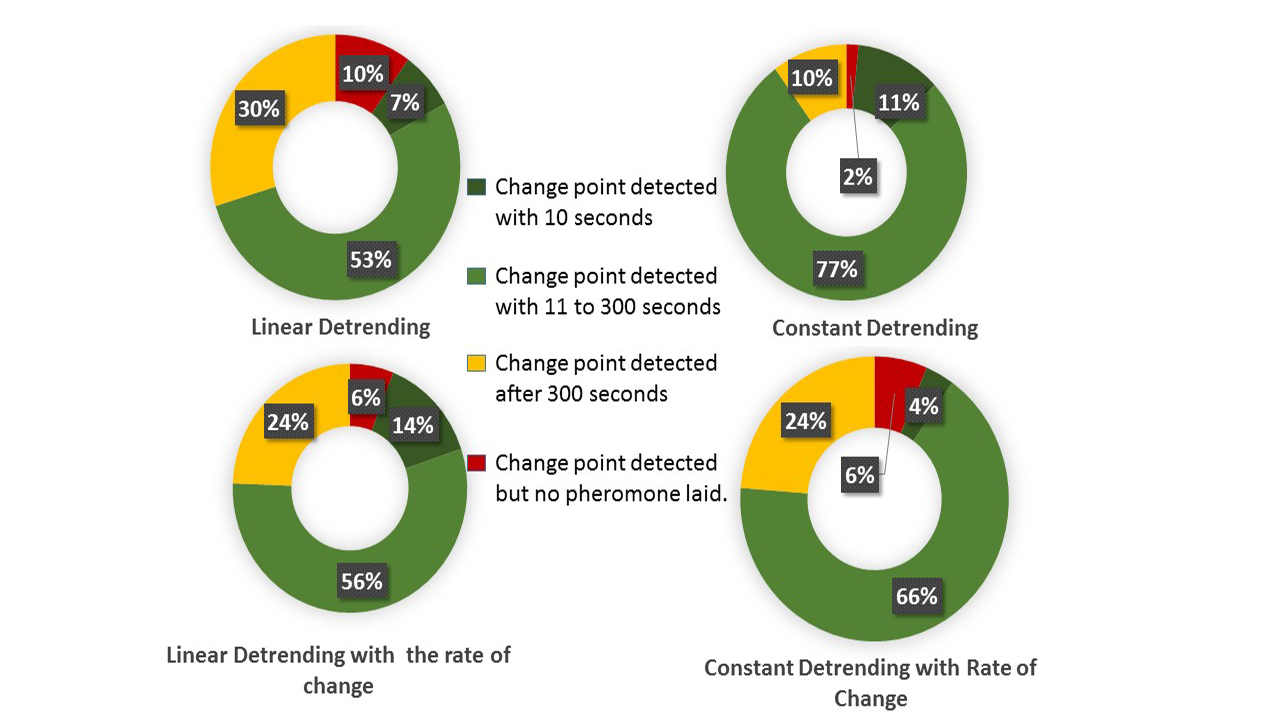
\includegraphics[height=0.35\textheight]{MaricopaDonutCharts/Slide23.JPG}
	\caption{Efficiency chart for \textit{P. Maricopa}, four pile,  communication only setting.}
\end{figure}
\begin{figure}[h]
	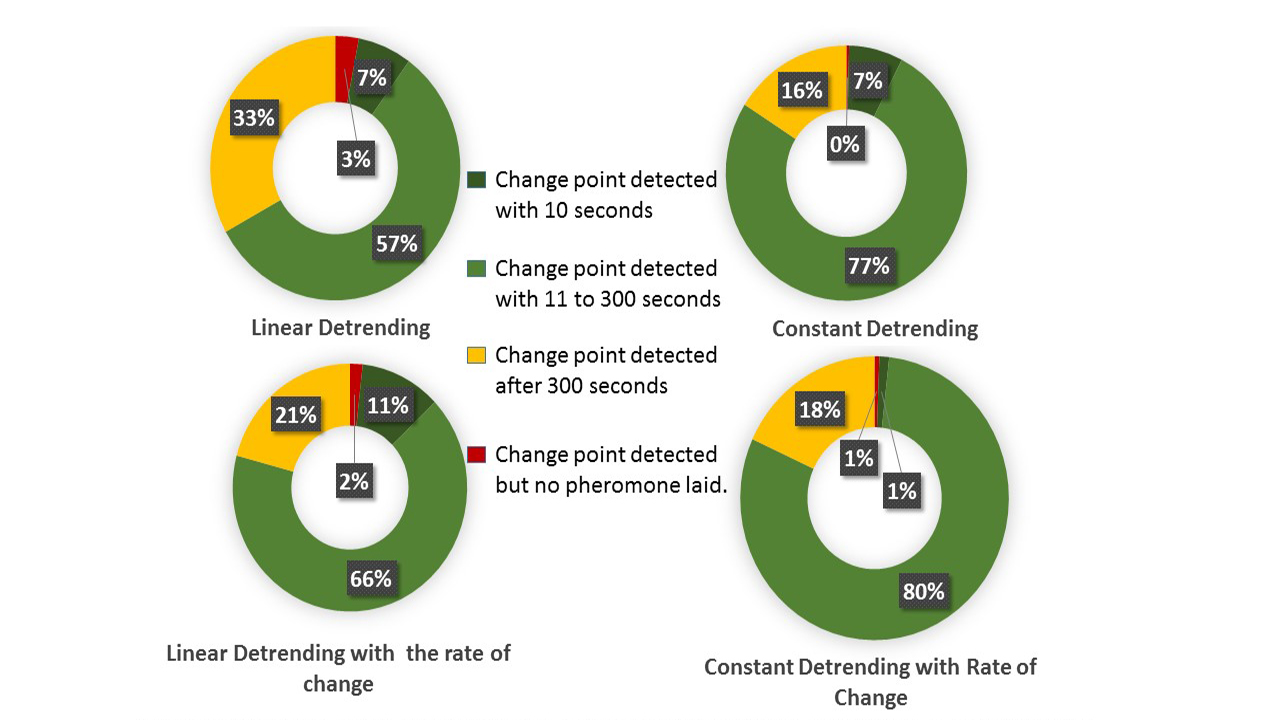
\includegraphics[height=0.35\textheight]{MaricopaDonutCharts/Slide24.JPG}
	\caption{Efficiency chart for \textit{P. Maricopa}, sixteen pile,  communication only setting.}
\end{figure}
\begin{figure}[h]
	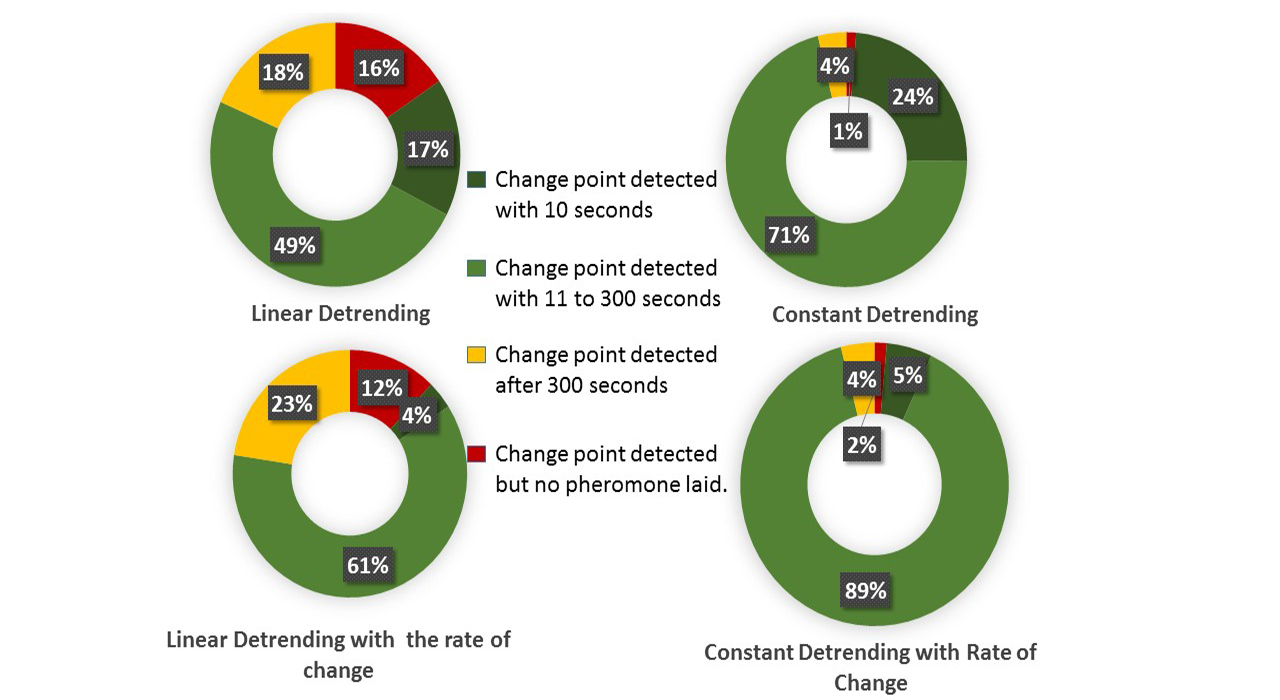
\includegraphics[height=0.35\textheight]{MaricopaDonutCharts/Slide25.JPG}
	\caption{Efficiency chart for \textit{P. Maricopa}, one pile,  memory and communication combined setting.}
\end{figure}
\begin{figure}[h]
	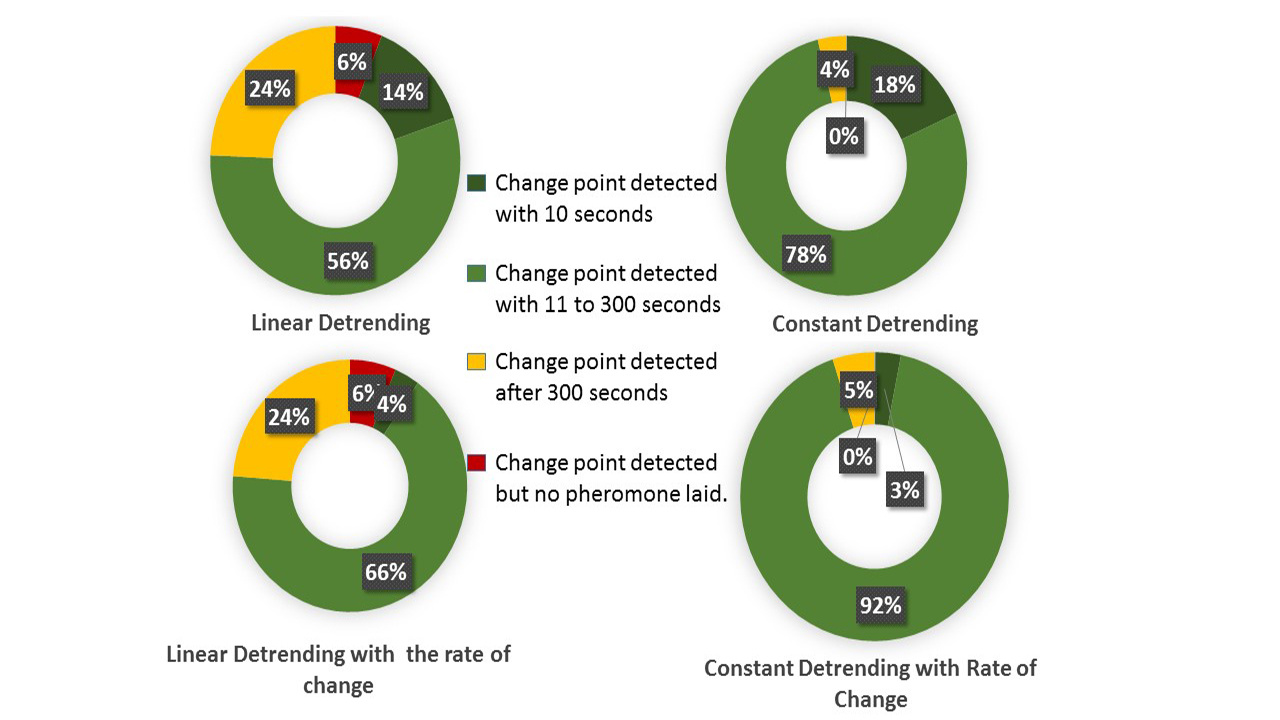
\includegraphics[height=0.35\textheight]{MaricopaDonutCharts/Slide26.JPG}
	\caption{Efficiency chart for \textit{P. Maricopa}, four pile, memory and communication combined setting.}
\end{figure}
\begin{figure}[h]
	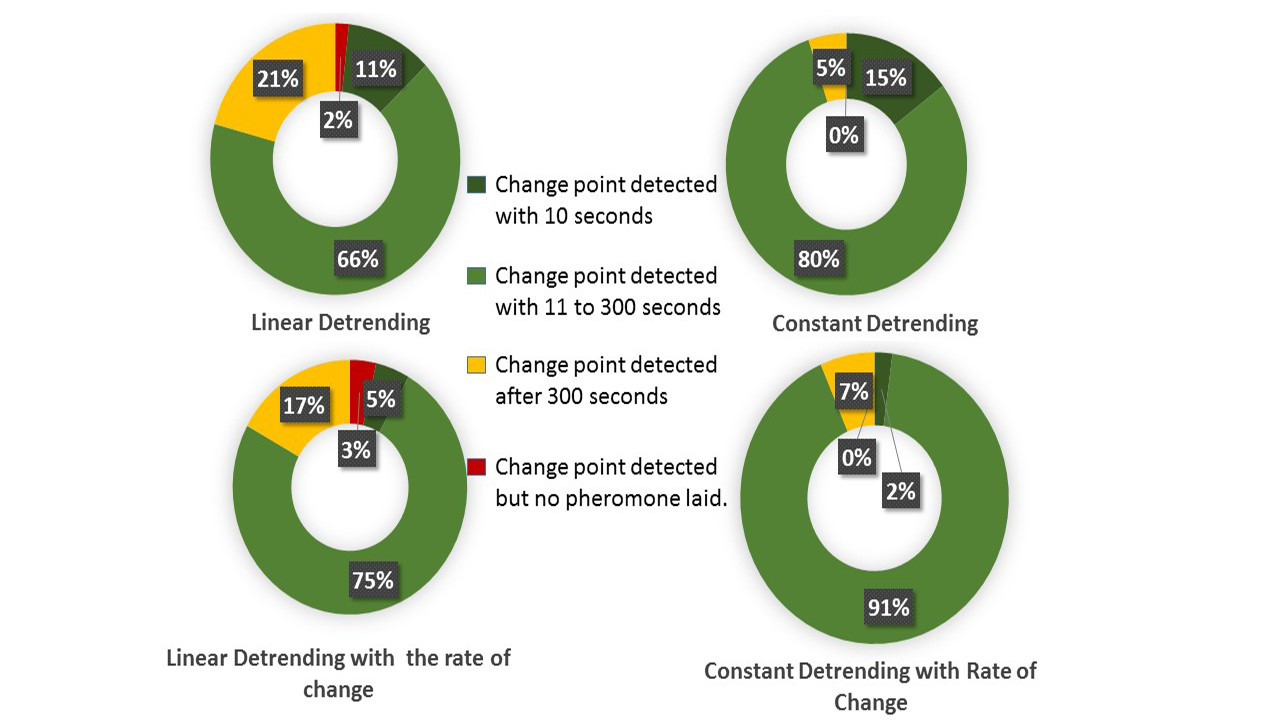
\includegraphics[height=0.35\textheight]{MaricopaDonutCharts/Slide27.JPG}
	\caption{Efficiency chart for \textit{P. Maricopa}, sixteen pile,  memory and communication combined setting.}
\end{figure}
\begin{figure}[h]
	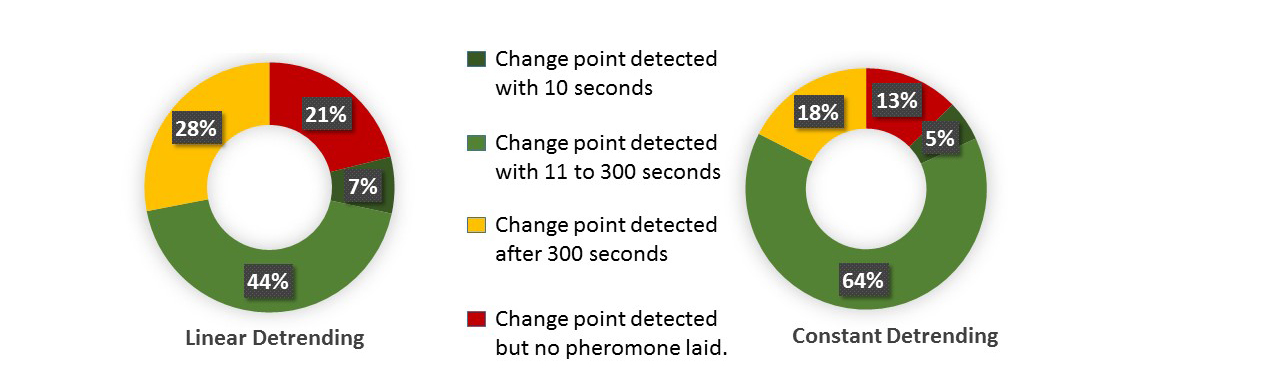
\includegraphics[width=\textwidth]{MaricopaDonutCharts/Slide28.JPG}
	\caption{Efficiency chart for \textit{P. Maricopa}, one pile,  memory only setting.}
\end{figure}
\begin{figure}[h]
	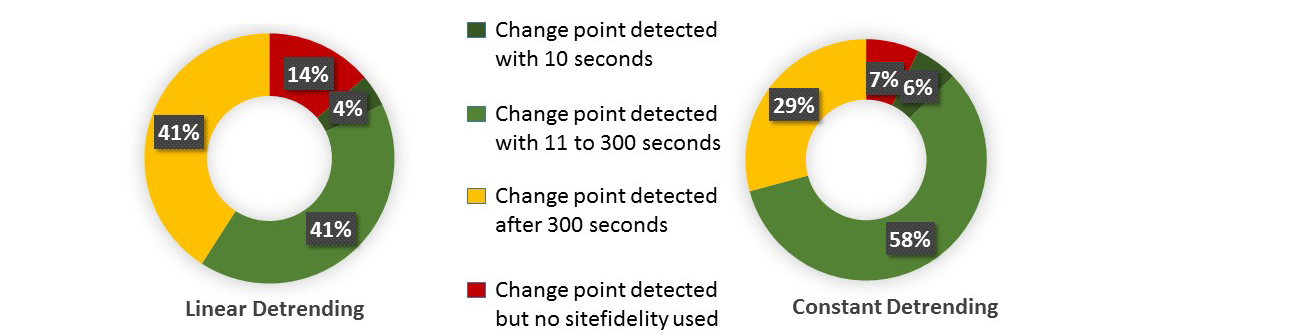
\includegraphics[width=\textwidth]{MaricopaDonutCharts/Slide29.JPG}
	\caption{Efficiency chart for \textit{P. Maricopa}, four pile,  memory only setting.}
\end{figure}
\begin{figure}[h]
	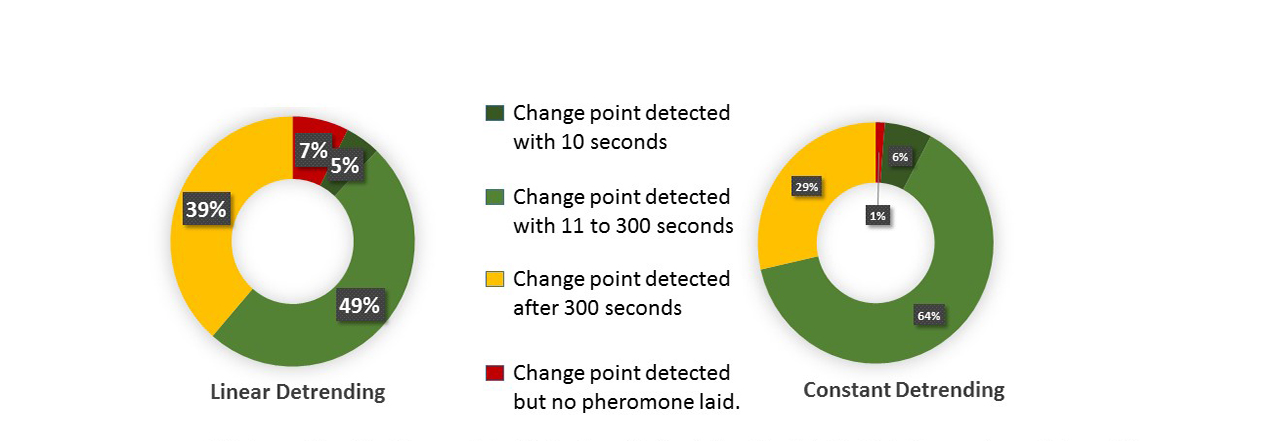
\includegraphics[width=\textwidth]{MaricopaDonutCharts/Slide30.JPG}
	\caption{Efficiency chart for \textit{P. Maricopa}, sixteen pile,  memory only setting.}
\end{figure}
\clearpage
\begin{figure}
	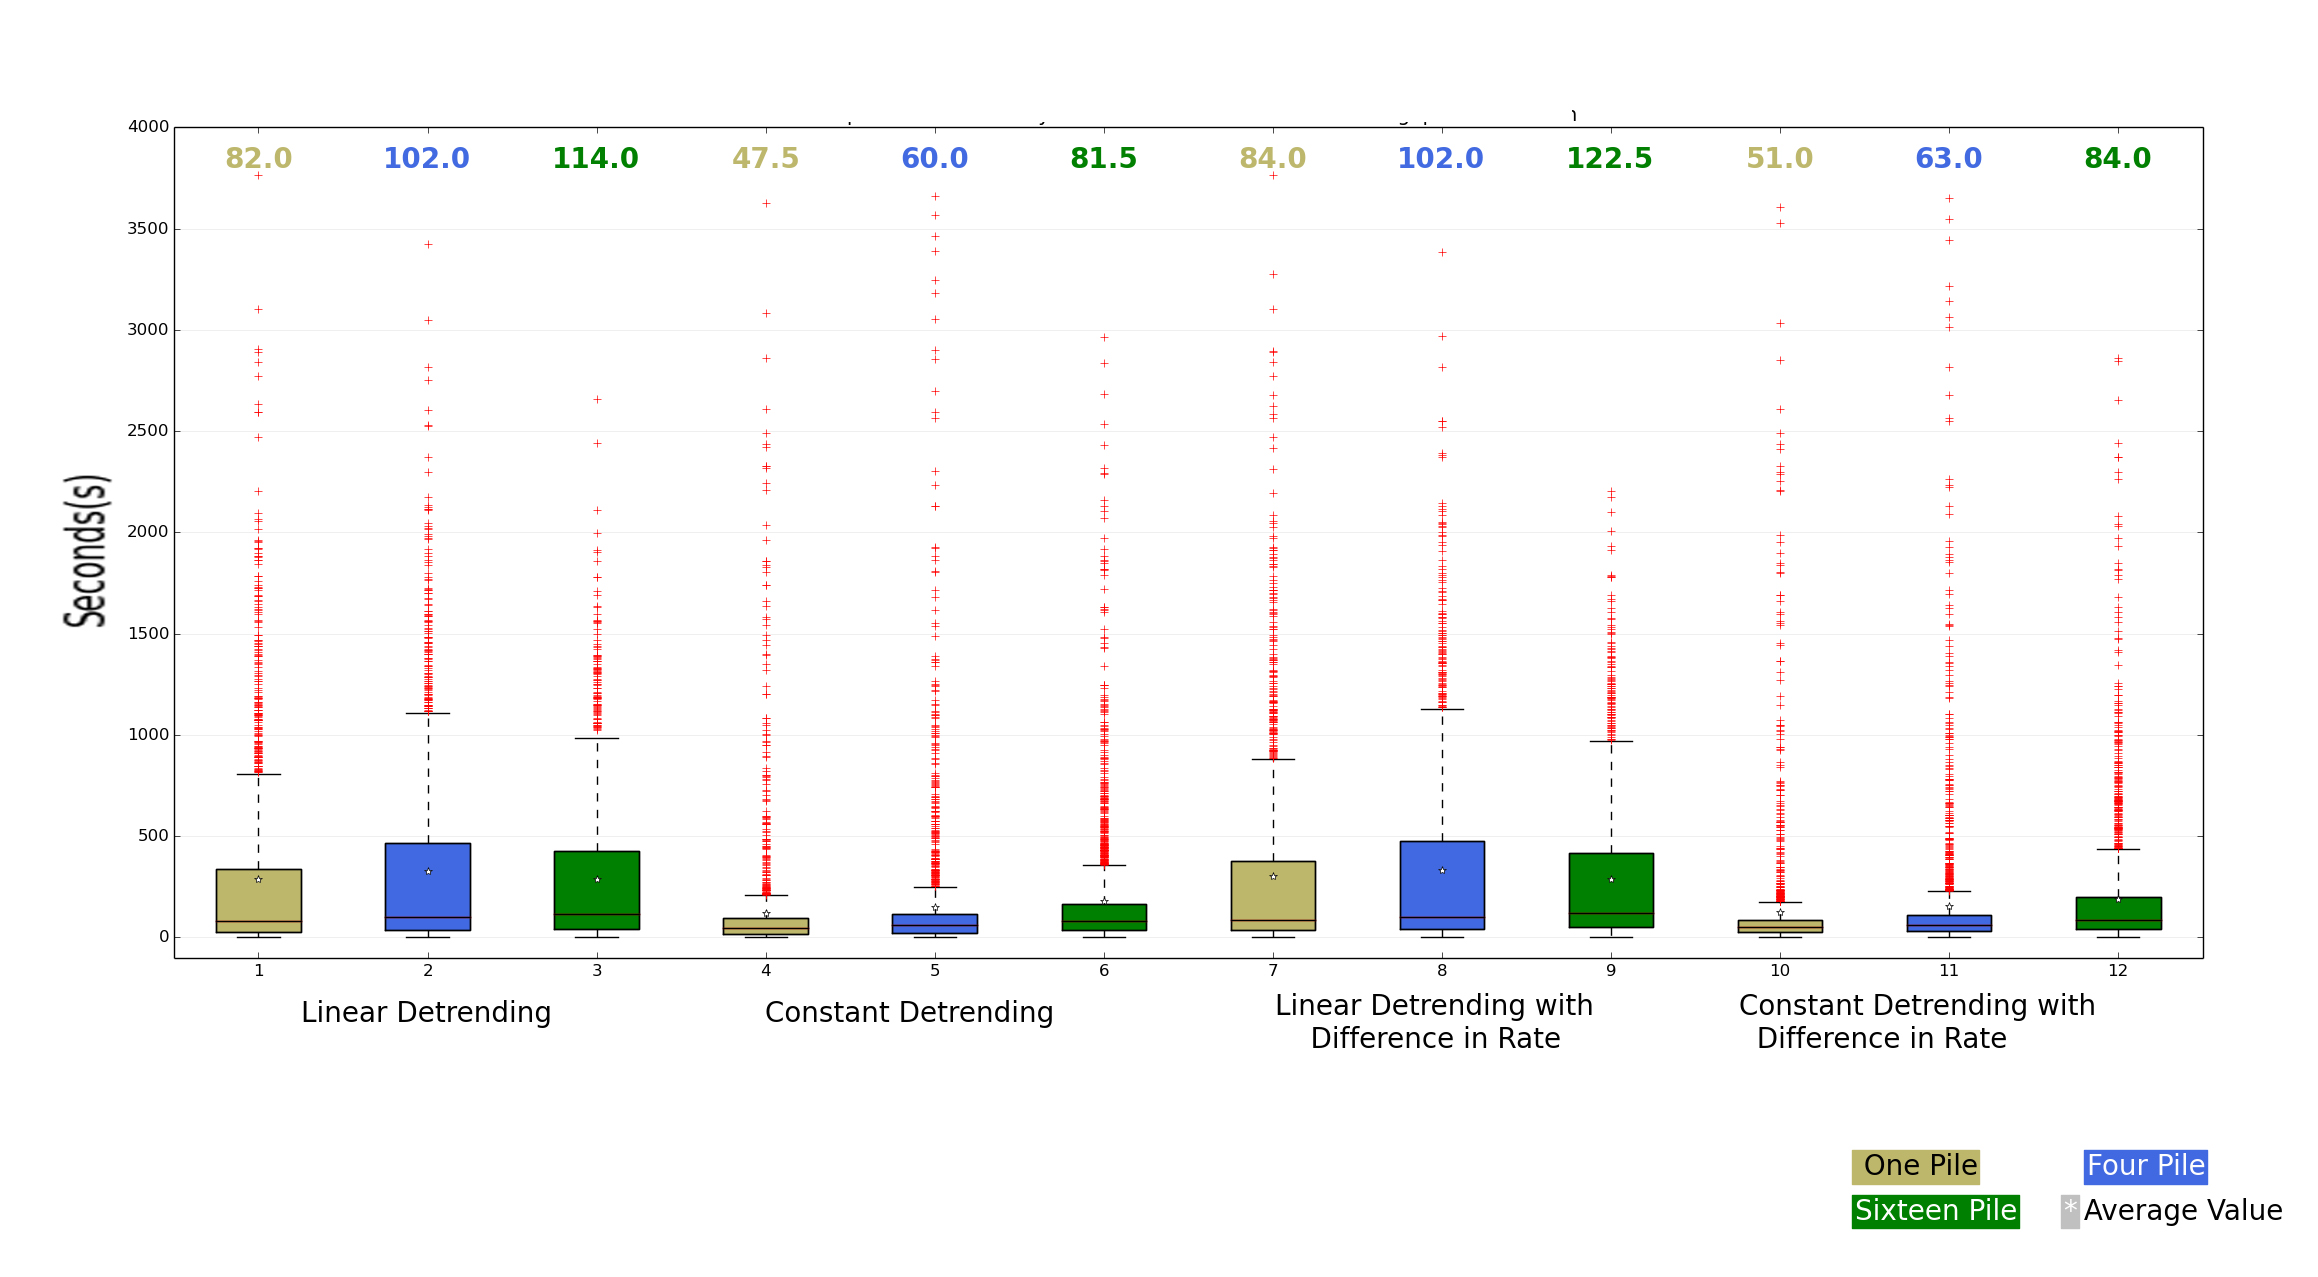
\includegraphics[width=\textwidth,height=0.35\textheight]{PheromoneOnly/PheromoneOnly.jpg}
	\caption{Comparison of change point detection methods for pheromone only parameters for \textit{P. Rugosus}. The time in seconds represents the difference between a pheromone laying event followed by a detection of change point in the foraging rate.}
\end{figure}
\begin{figure}
	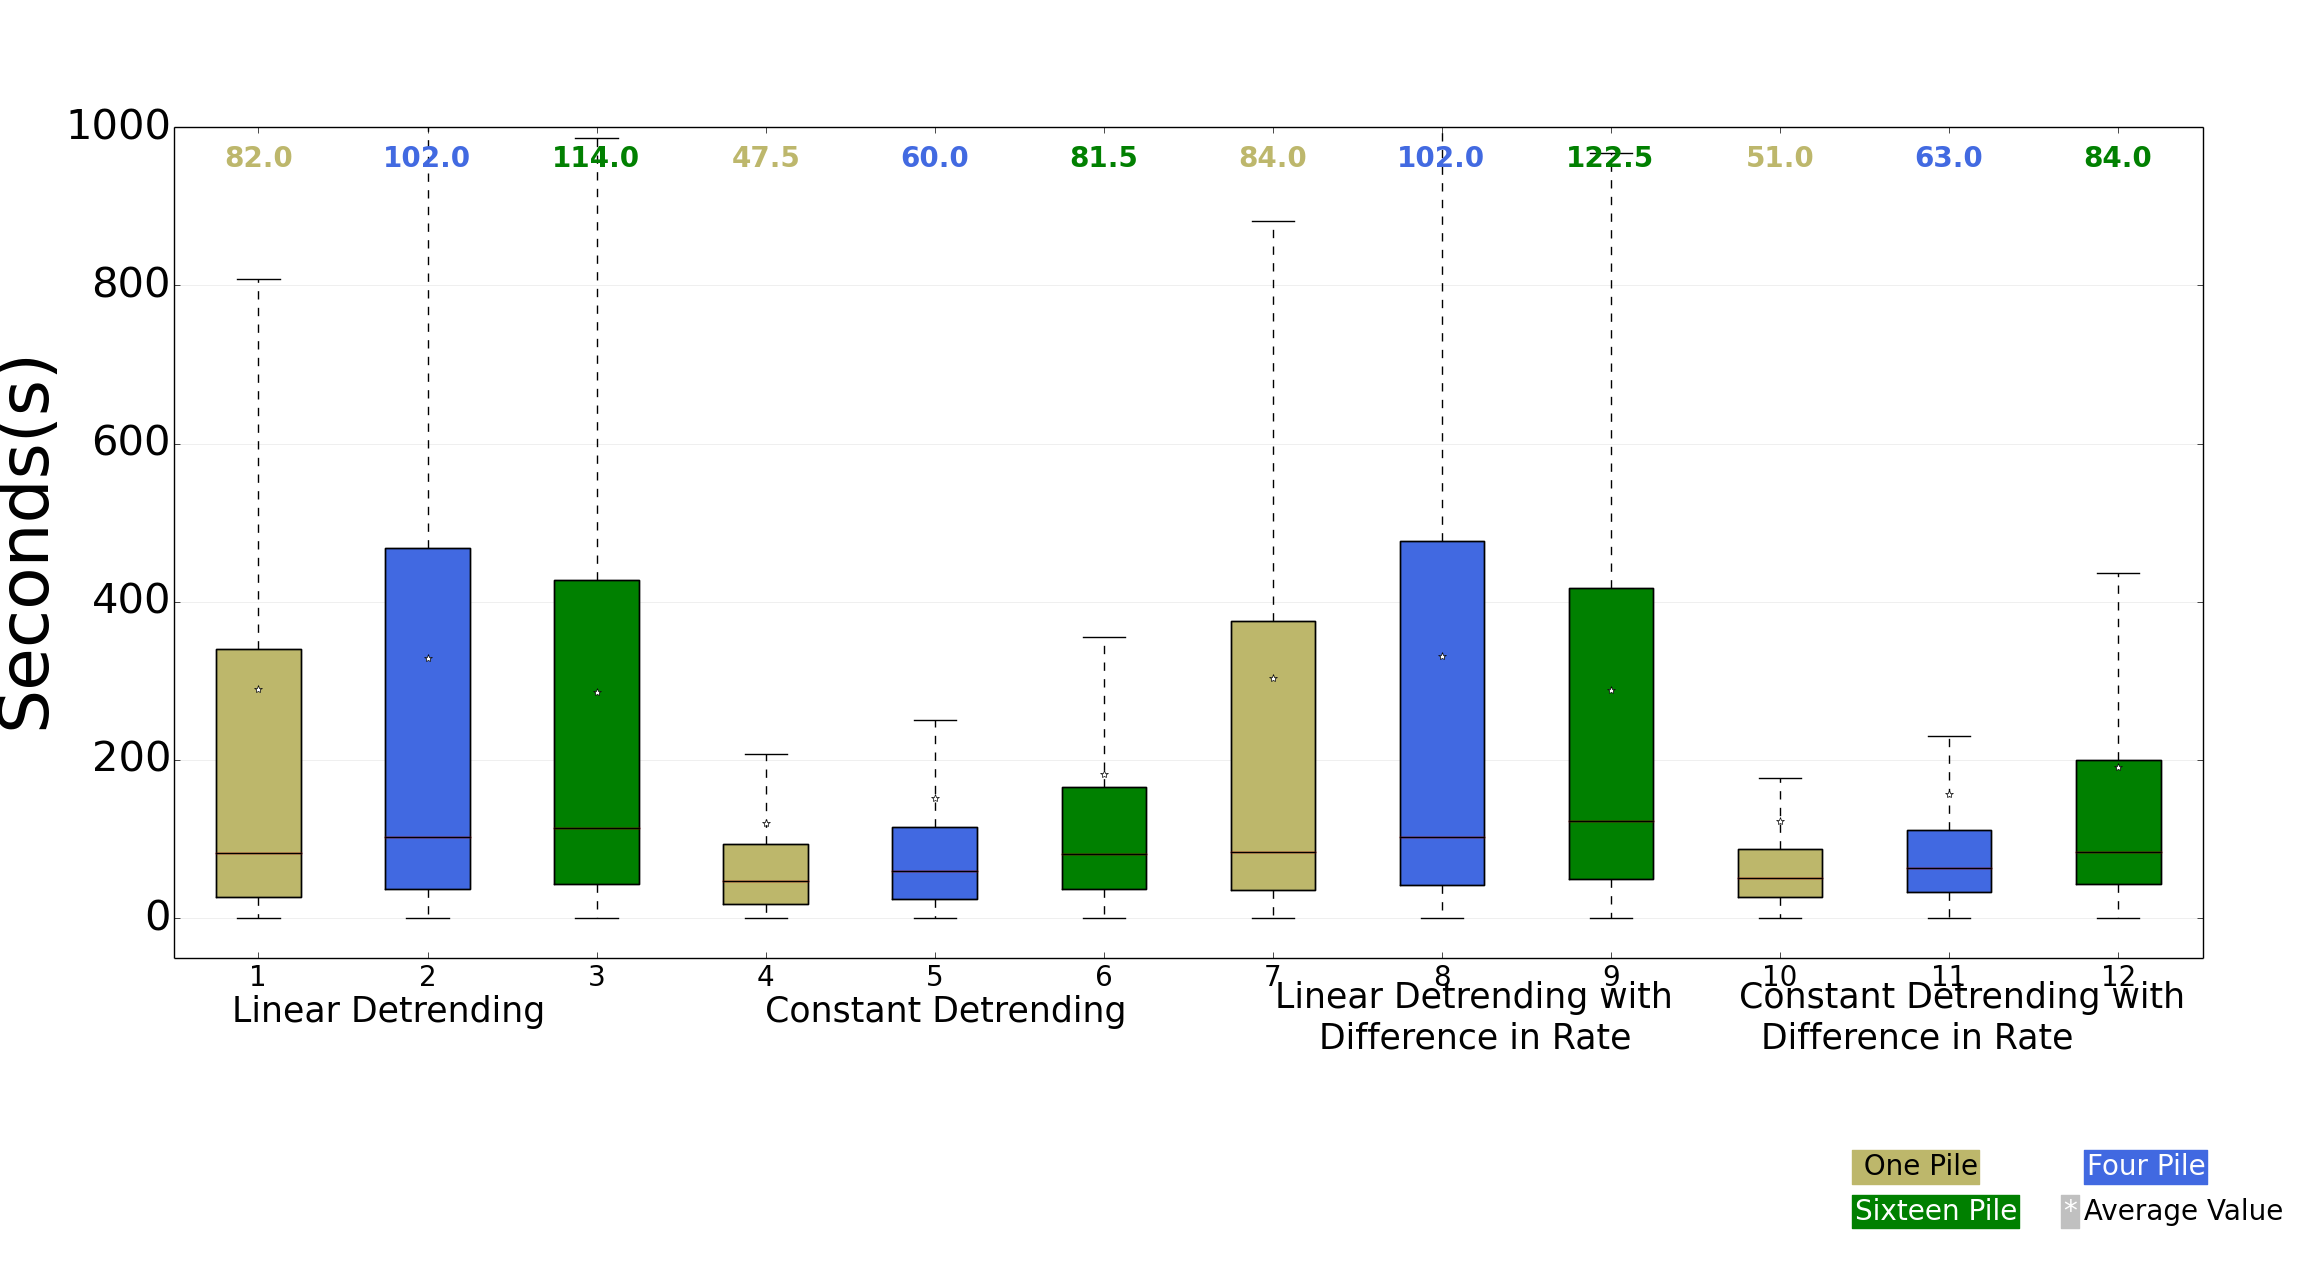
\includegraphics[width=\textwidth,height=0.35\textheight]{PheromoneOnly/AllPlot.png}
	\caption{Comparison of change point detection method without outliers for pheromone only parameters \textit{P. Rugosus}.The time in seconds represents the difference between a pheromone laying event followed by a detection of change point in the foraging rate.}
\end{figure}
\begin{figure}
	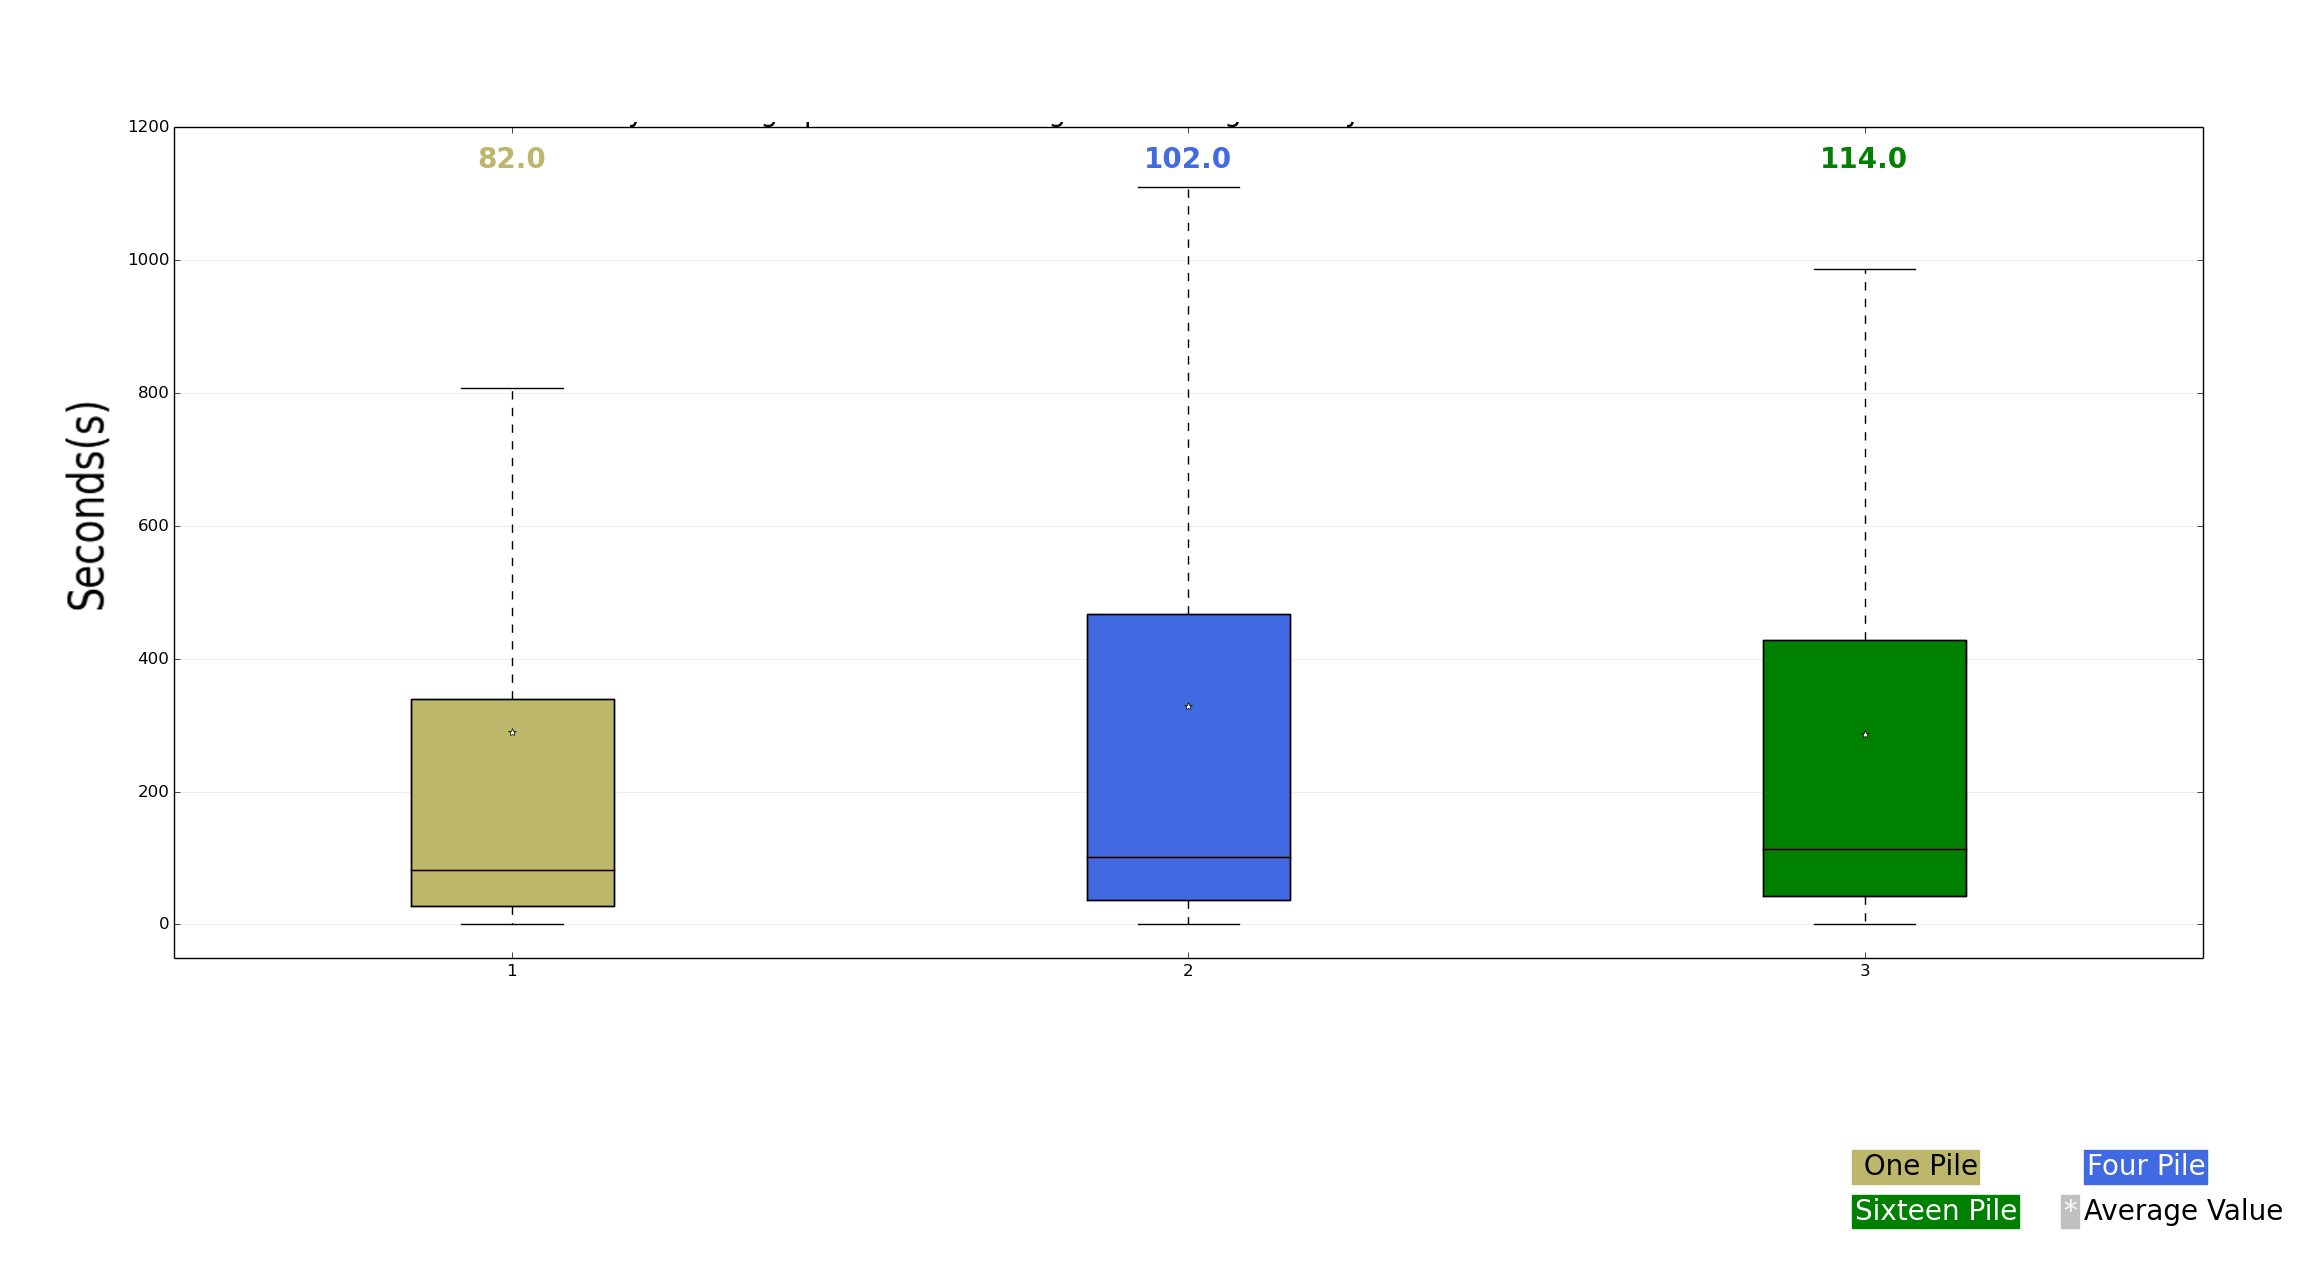
\includegraphics[width=\textwidth,height=0.35\textheight]{PheromoneOnly/Linear.png}
	\caption{Efficiency of Linear Detrending method on data of \textit{P. Rugosus} for pheromone only settings}
\end{figure}
\begin{figure}
	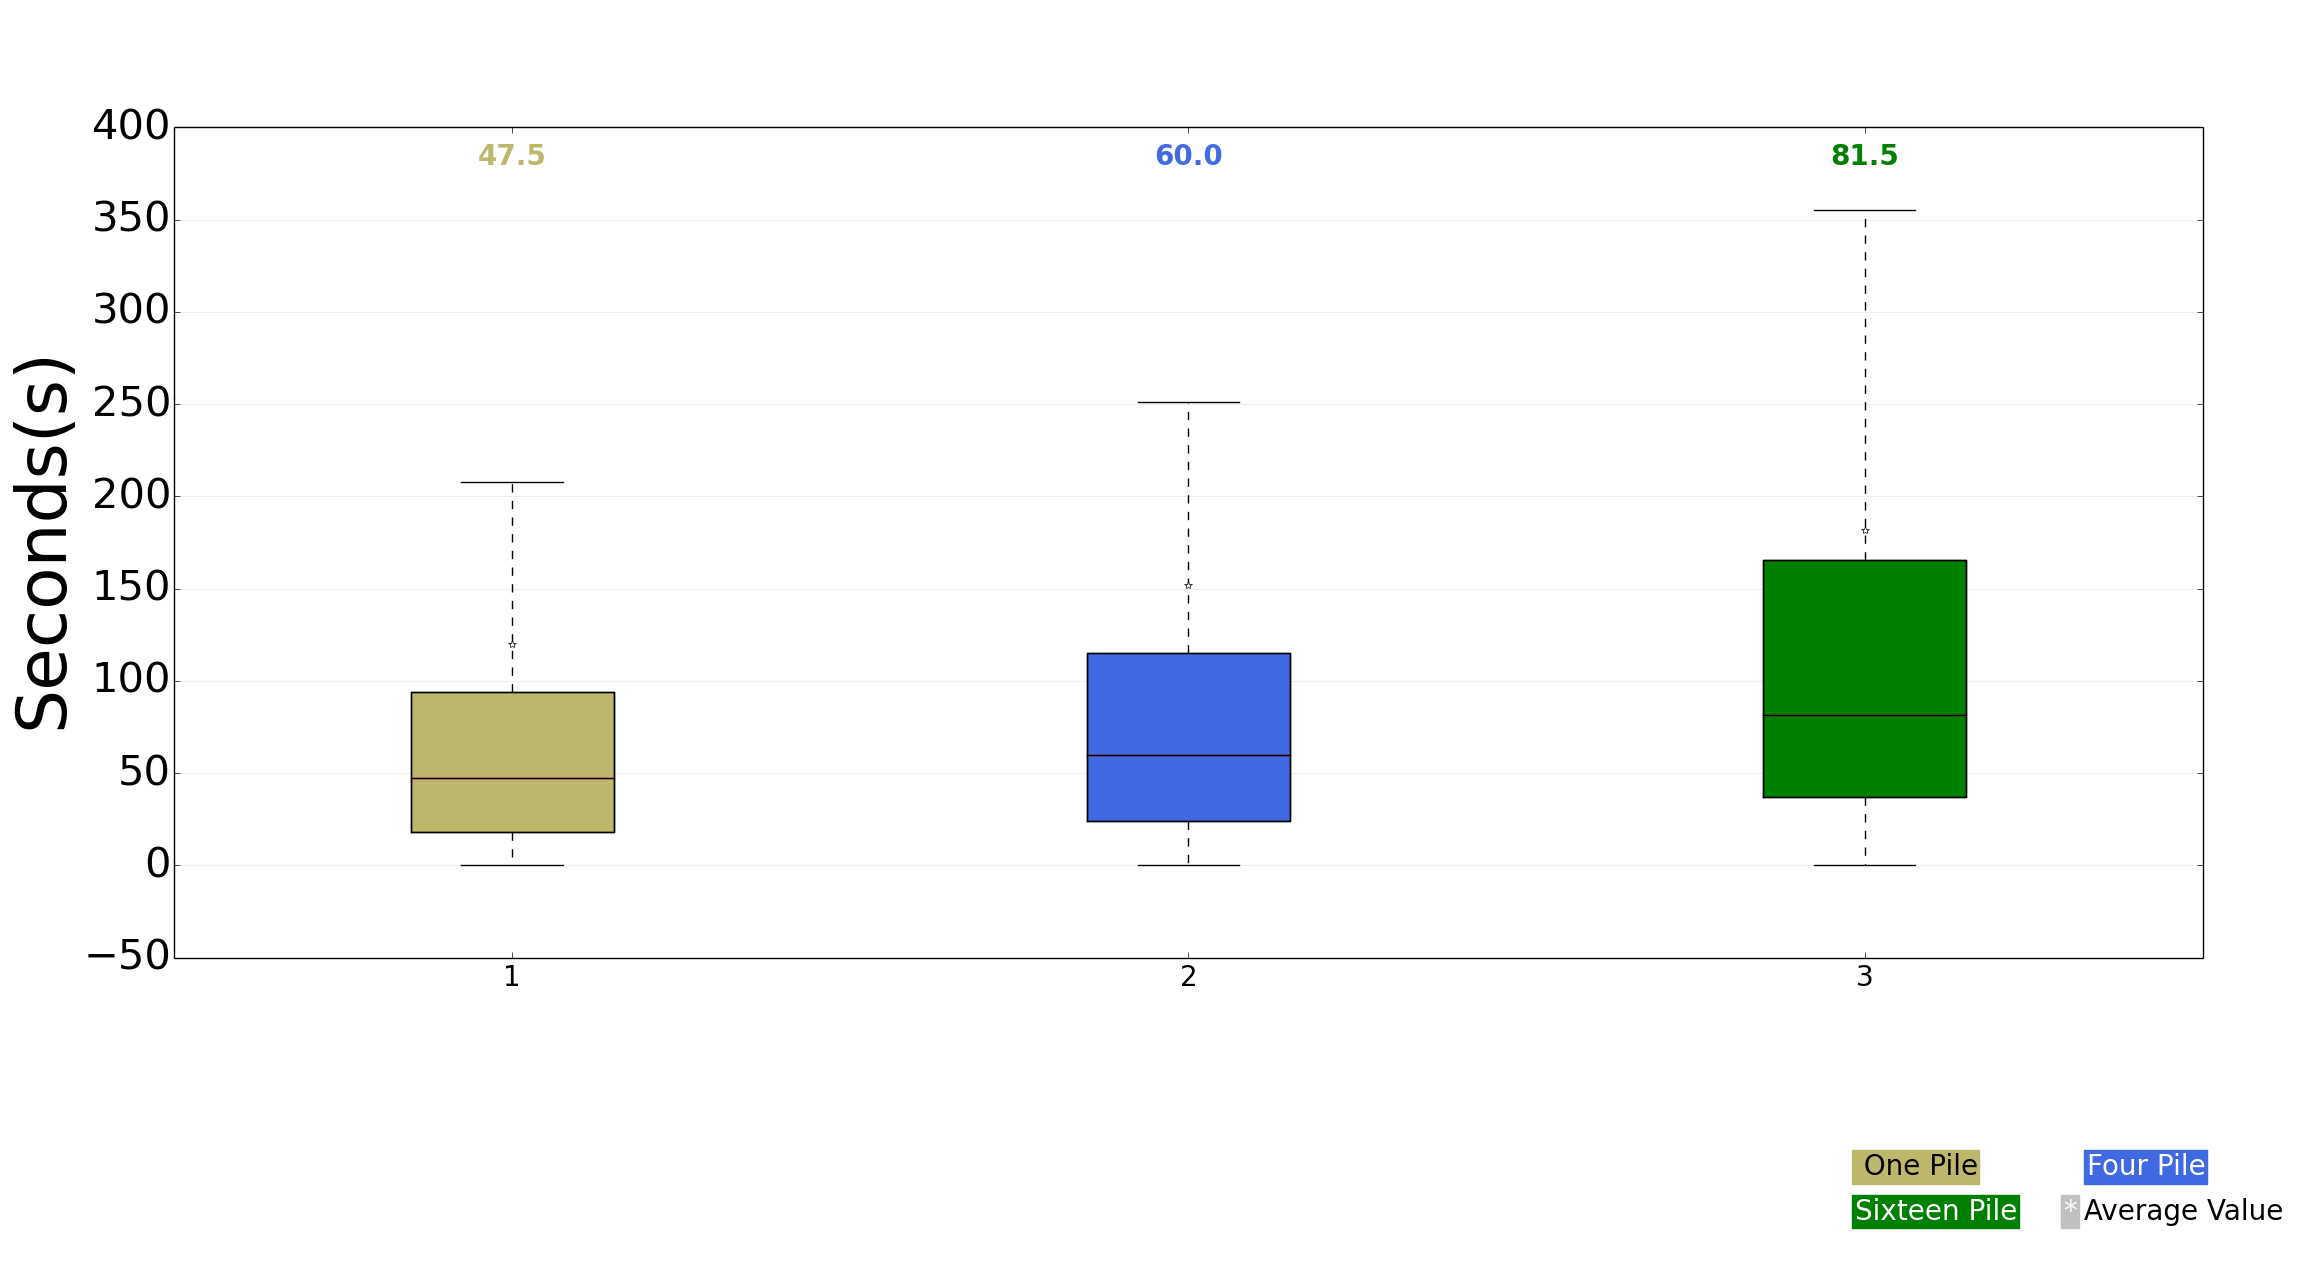
\includegraphics[width=\textwidth,height=0.35\textheight]{PheromoneOnly/ConstantWithNoOutlier.png}
	\caption{Efficiency of Constant Detrending method on data of \textit{P. Rugosus} for pheromone only Settings.}
\end{figure}
\begin{figure}
	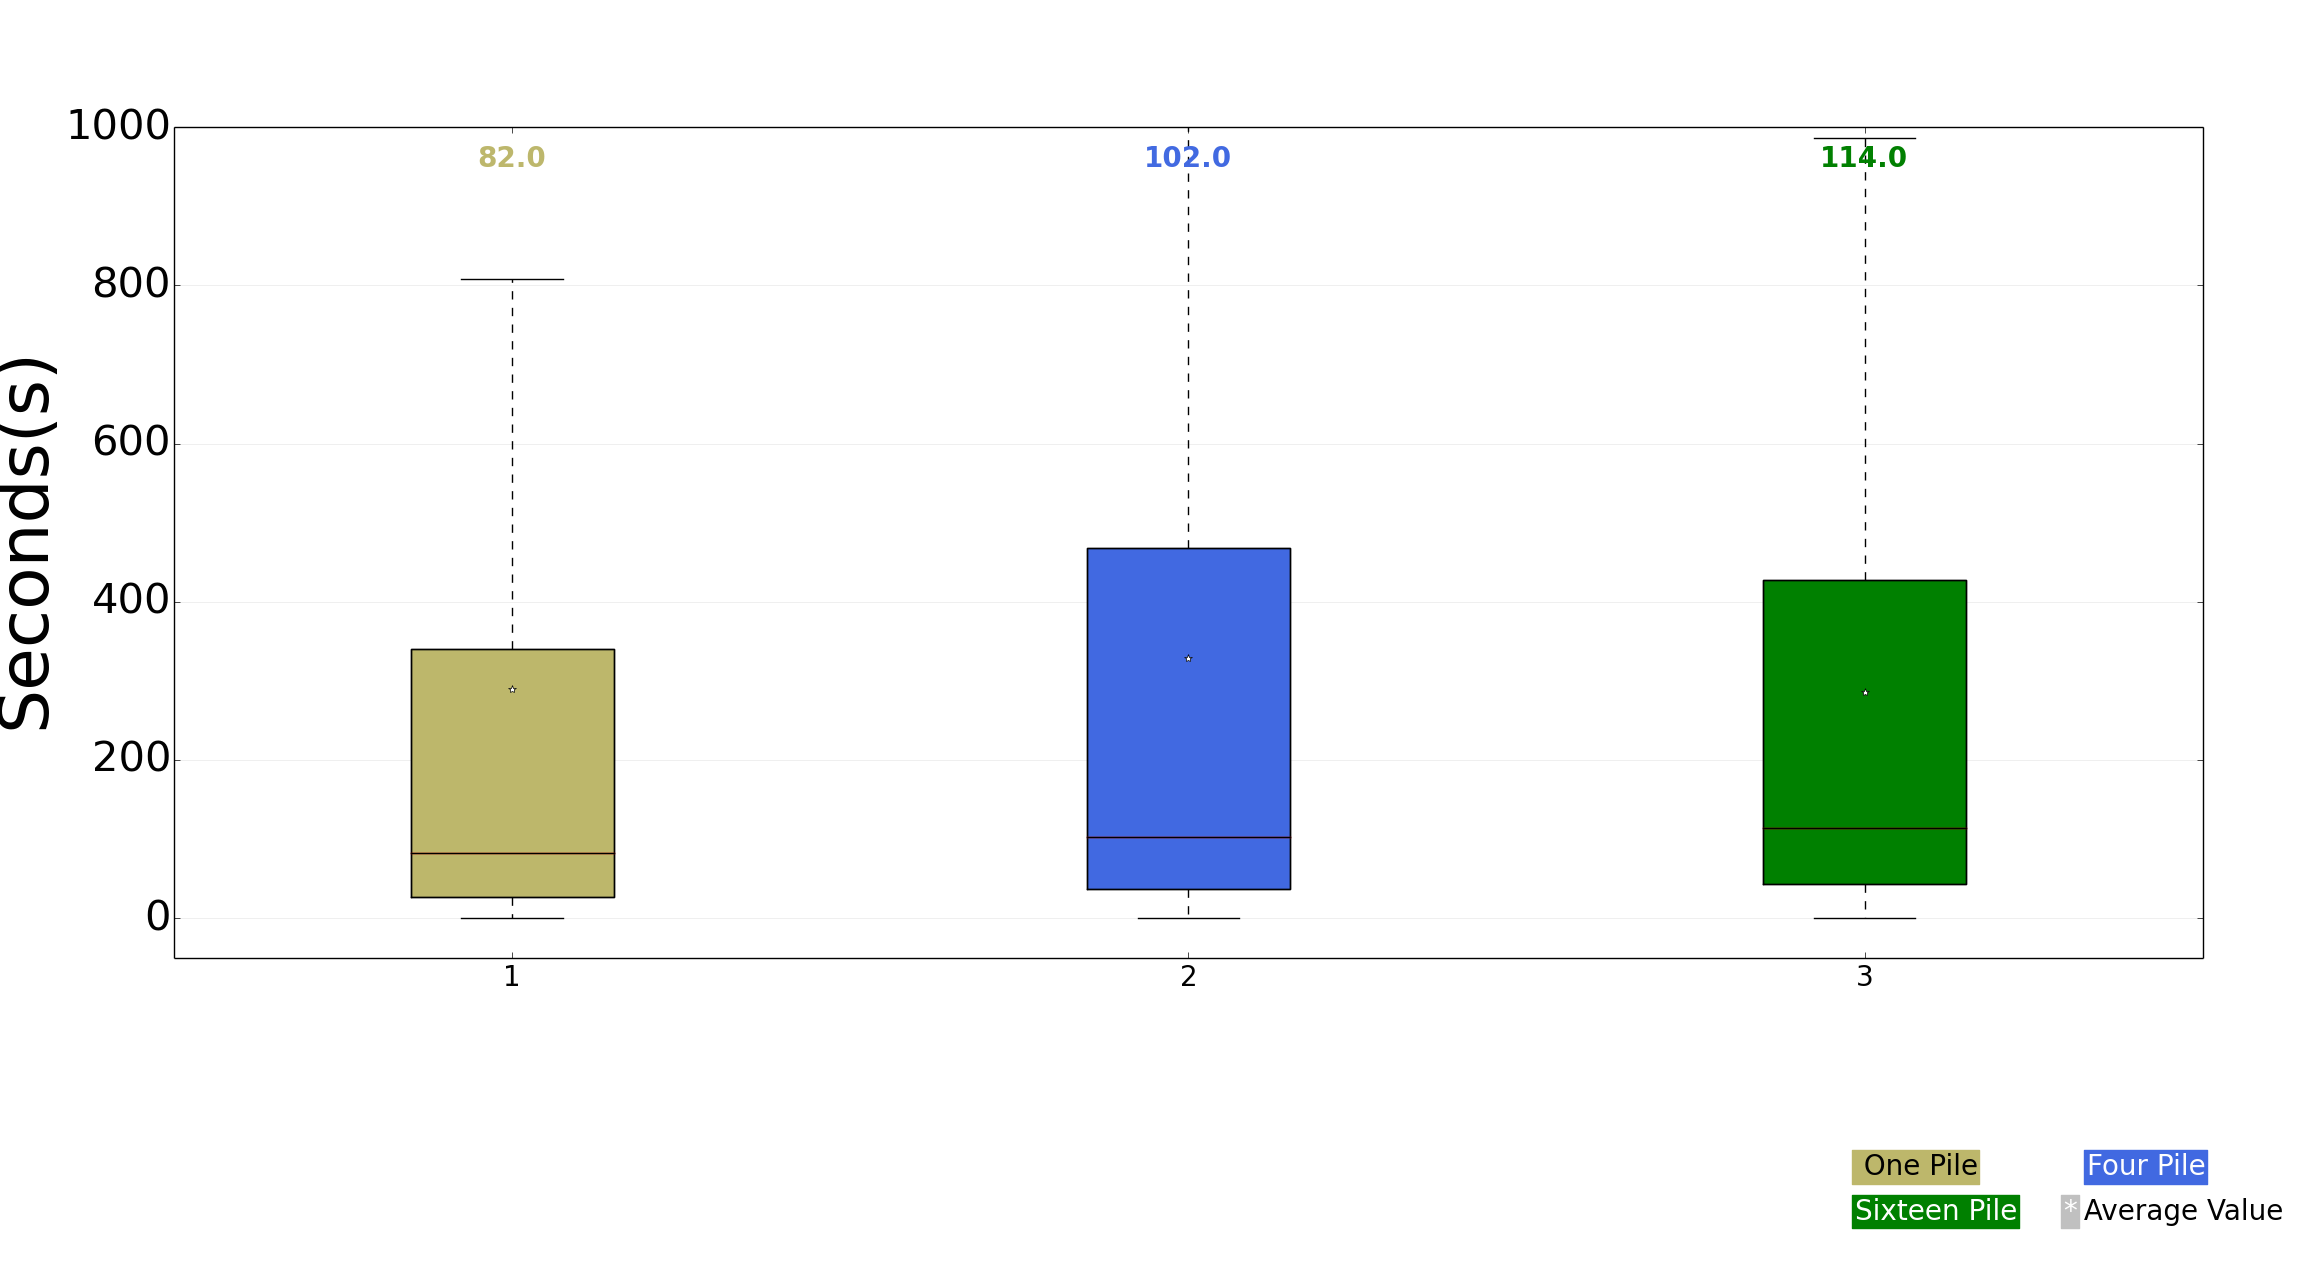
\includegraphics[width=\textwidth,height=0.35\textheight]{PheromoneOnly/LinearWithNoOutlierRateOfChange.png}
	\caption{Efficiency of Linear Detrending with rate of change method on data of \textit{P. Rugosus} for pheromone only settings.}
\end{figure}
\begin{figure}
	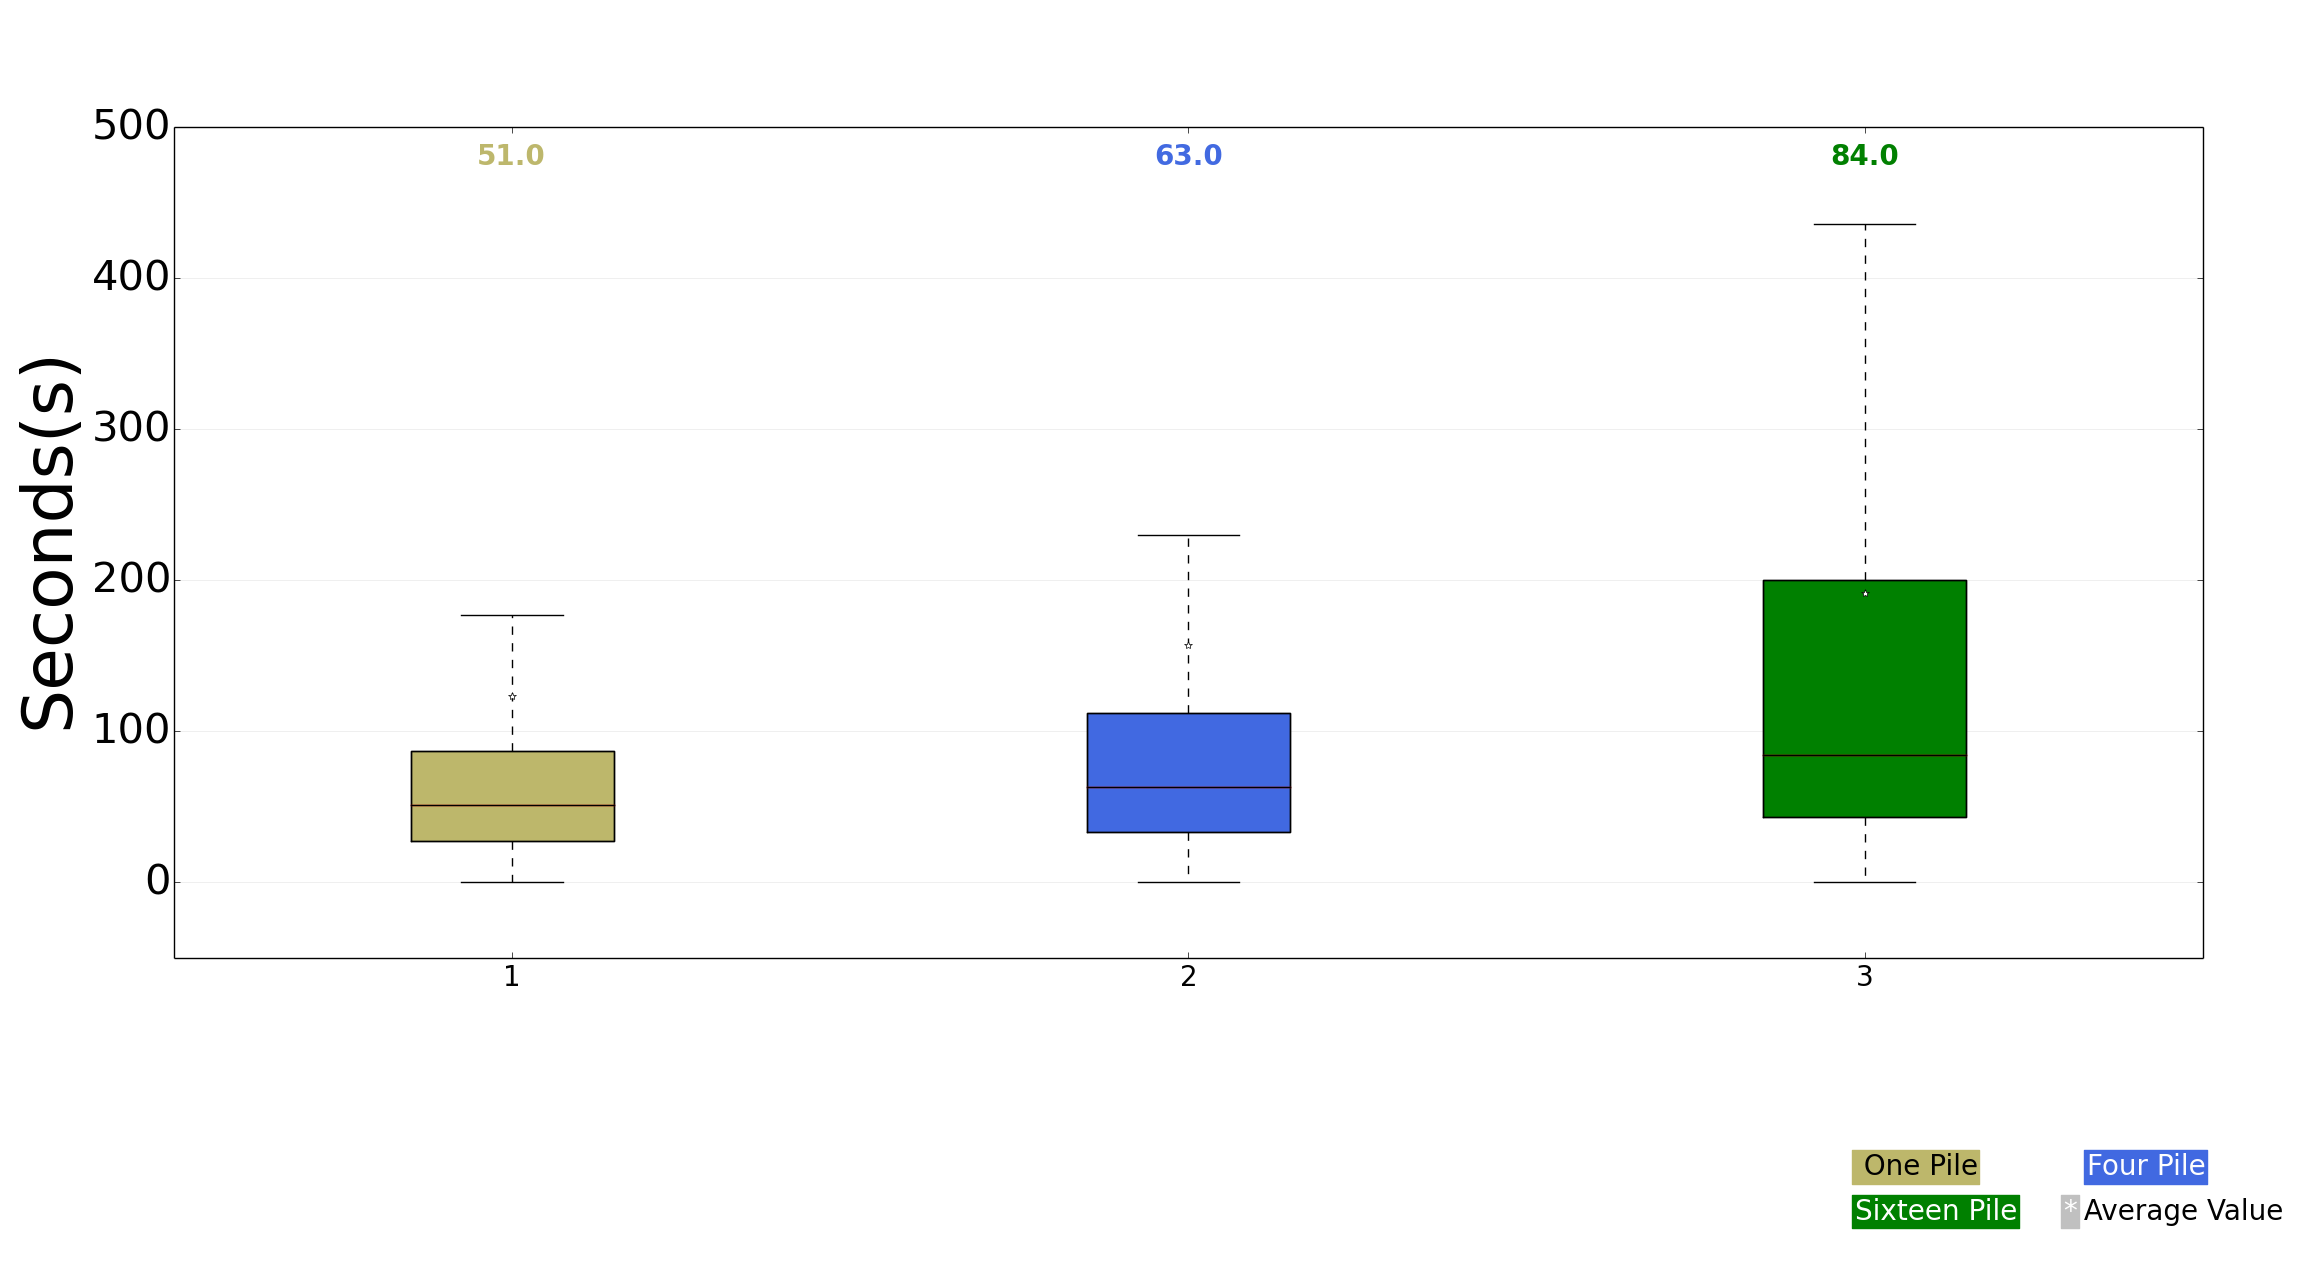
\includegraphics[width=\textwidth,height=0.35\textheight]{PheromoneOnly/ConsantWithNoOutlierRateOfChange.png}
	\caption{Efficiency of Linear Detrending with rate of change method on data of \textit{P. Rugosus} for pheromone only settings}
\end{figure}
\begin{figure}
	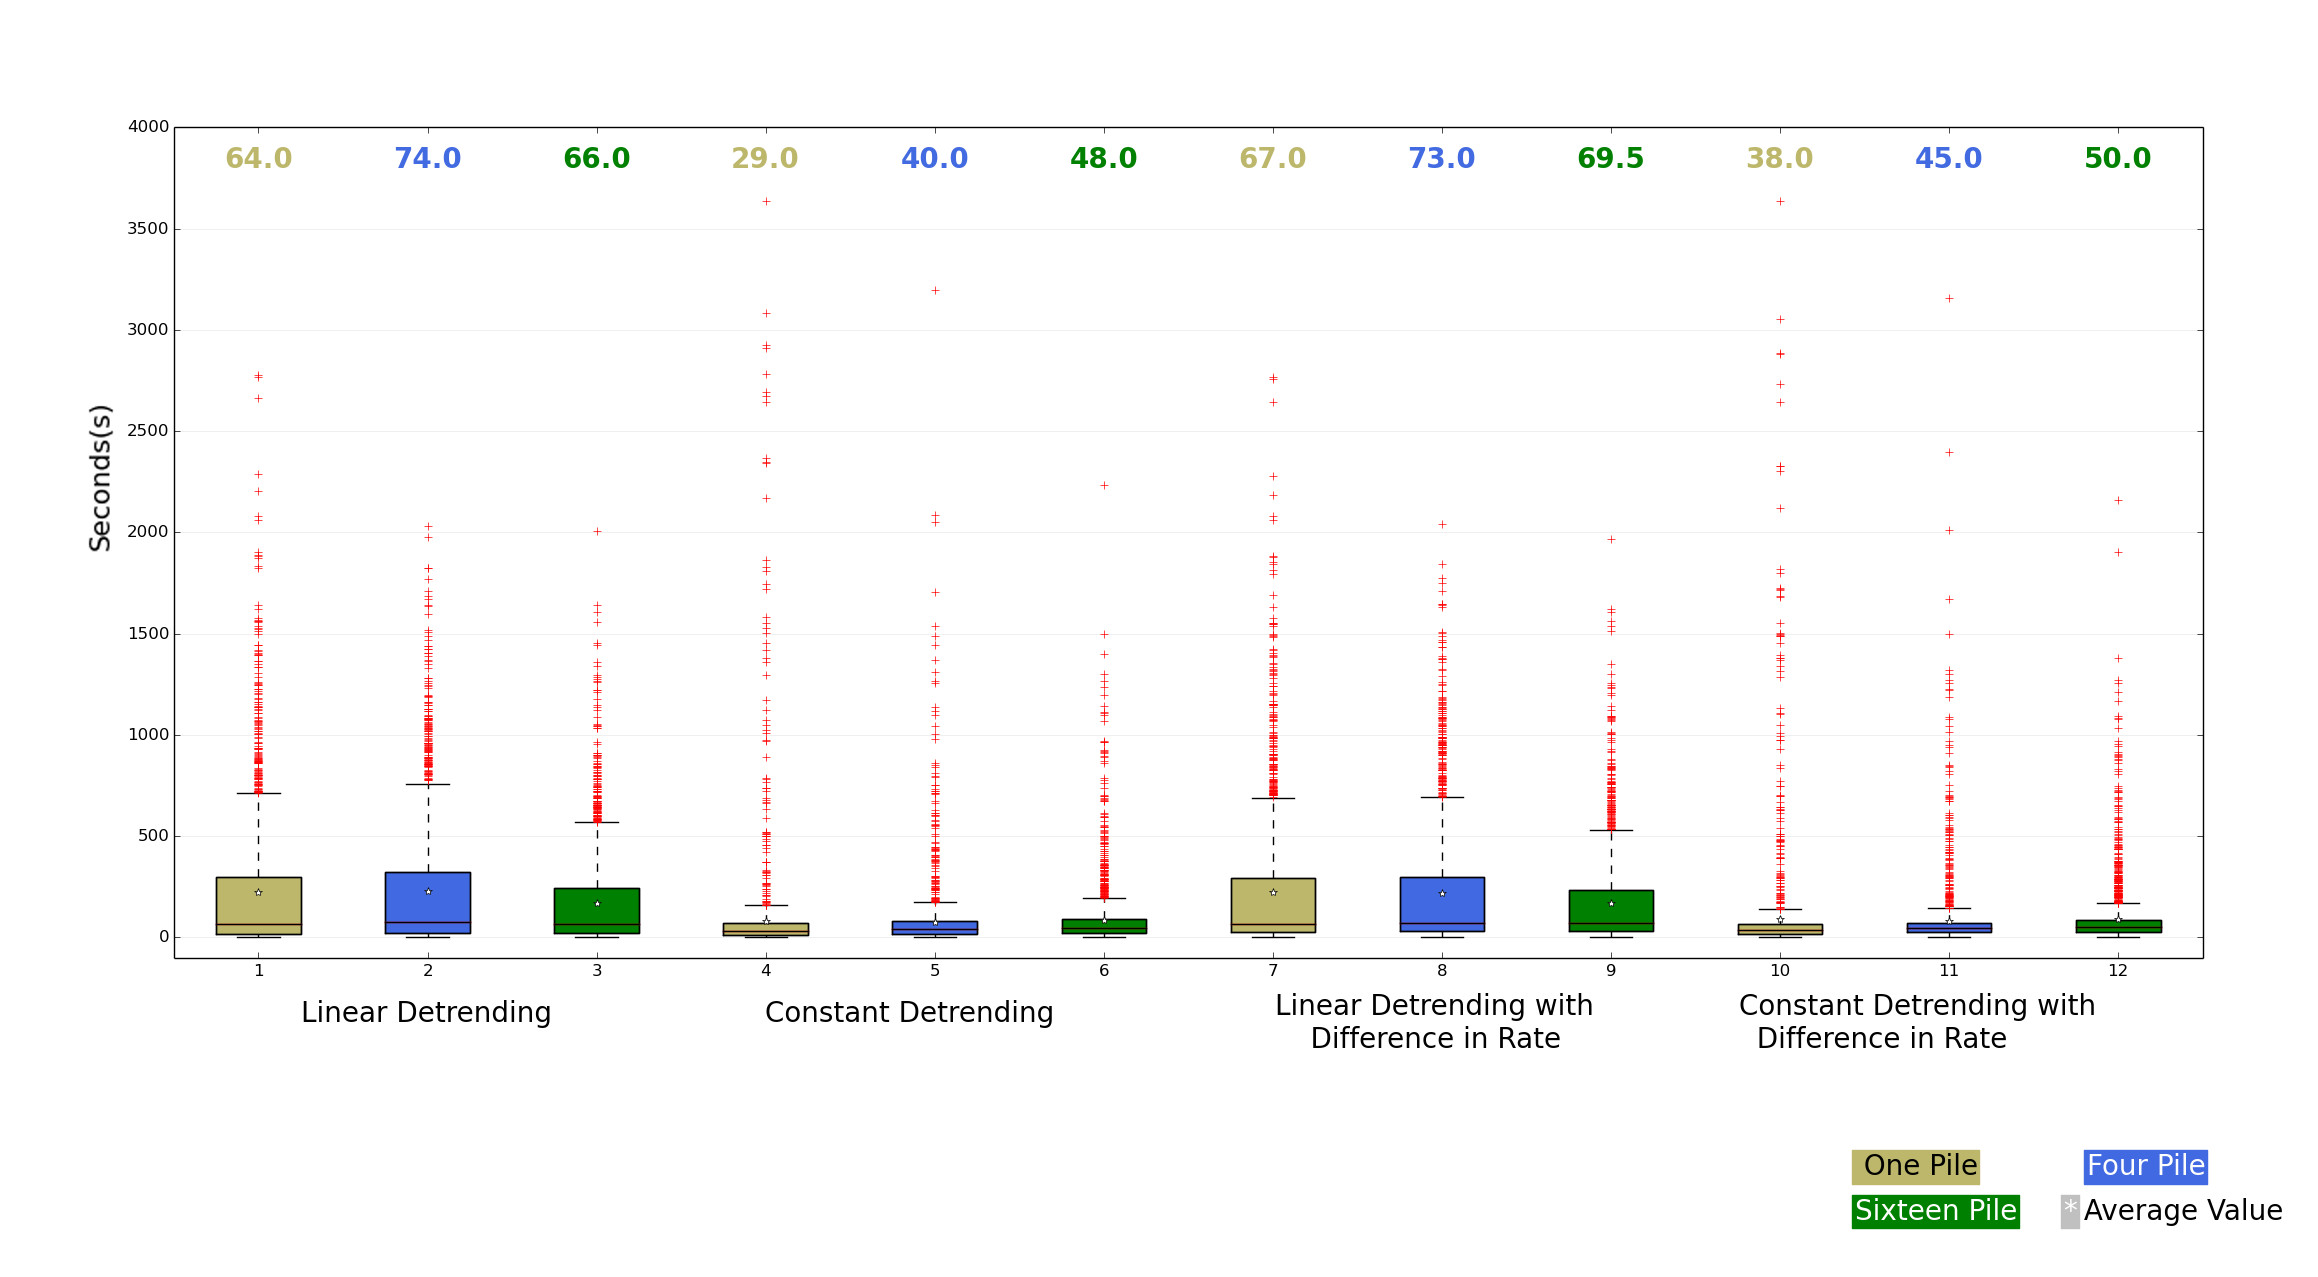
\includegraphics[width=\textwidth,height=0.35\textheight]{AllParameters/AllPlotComparison.png}
	\caption{Comparison of all methods on data of \textit{P. Rugosus} for both combination of communication and memory}
\end{figure}
\begin{figure}
	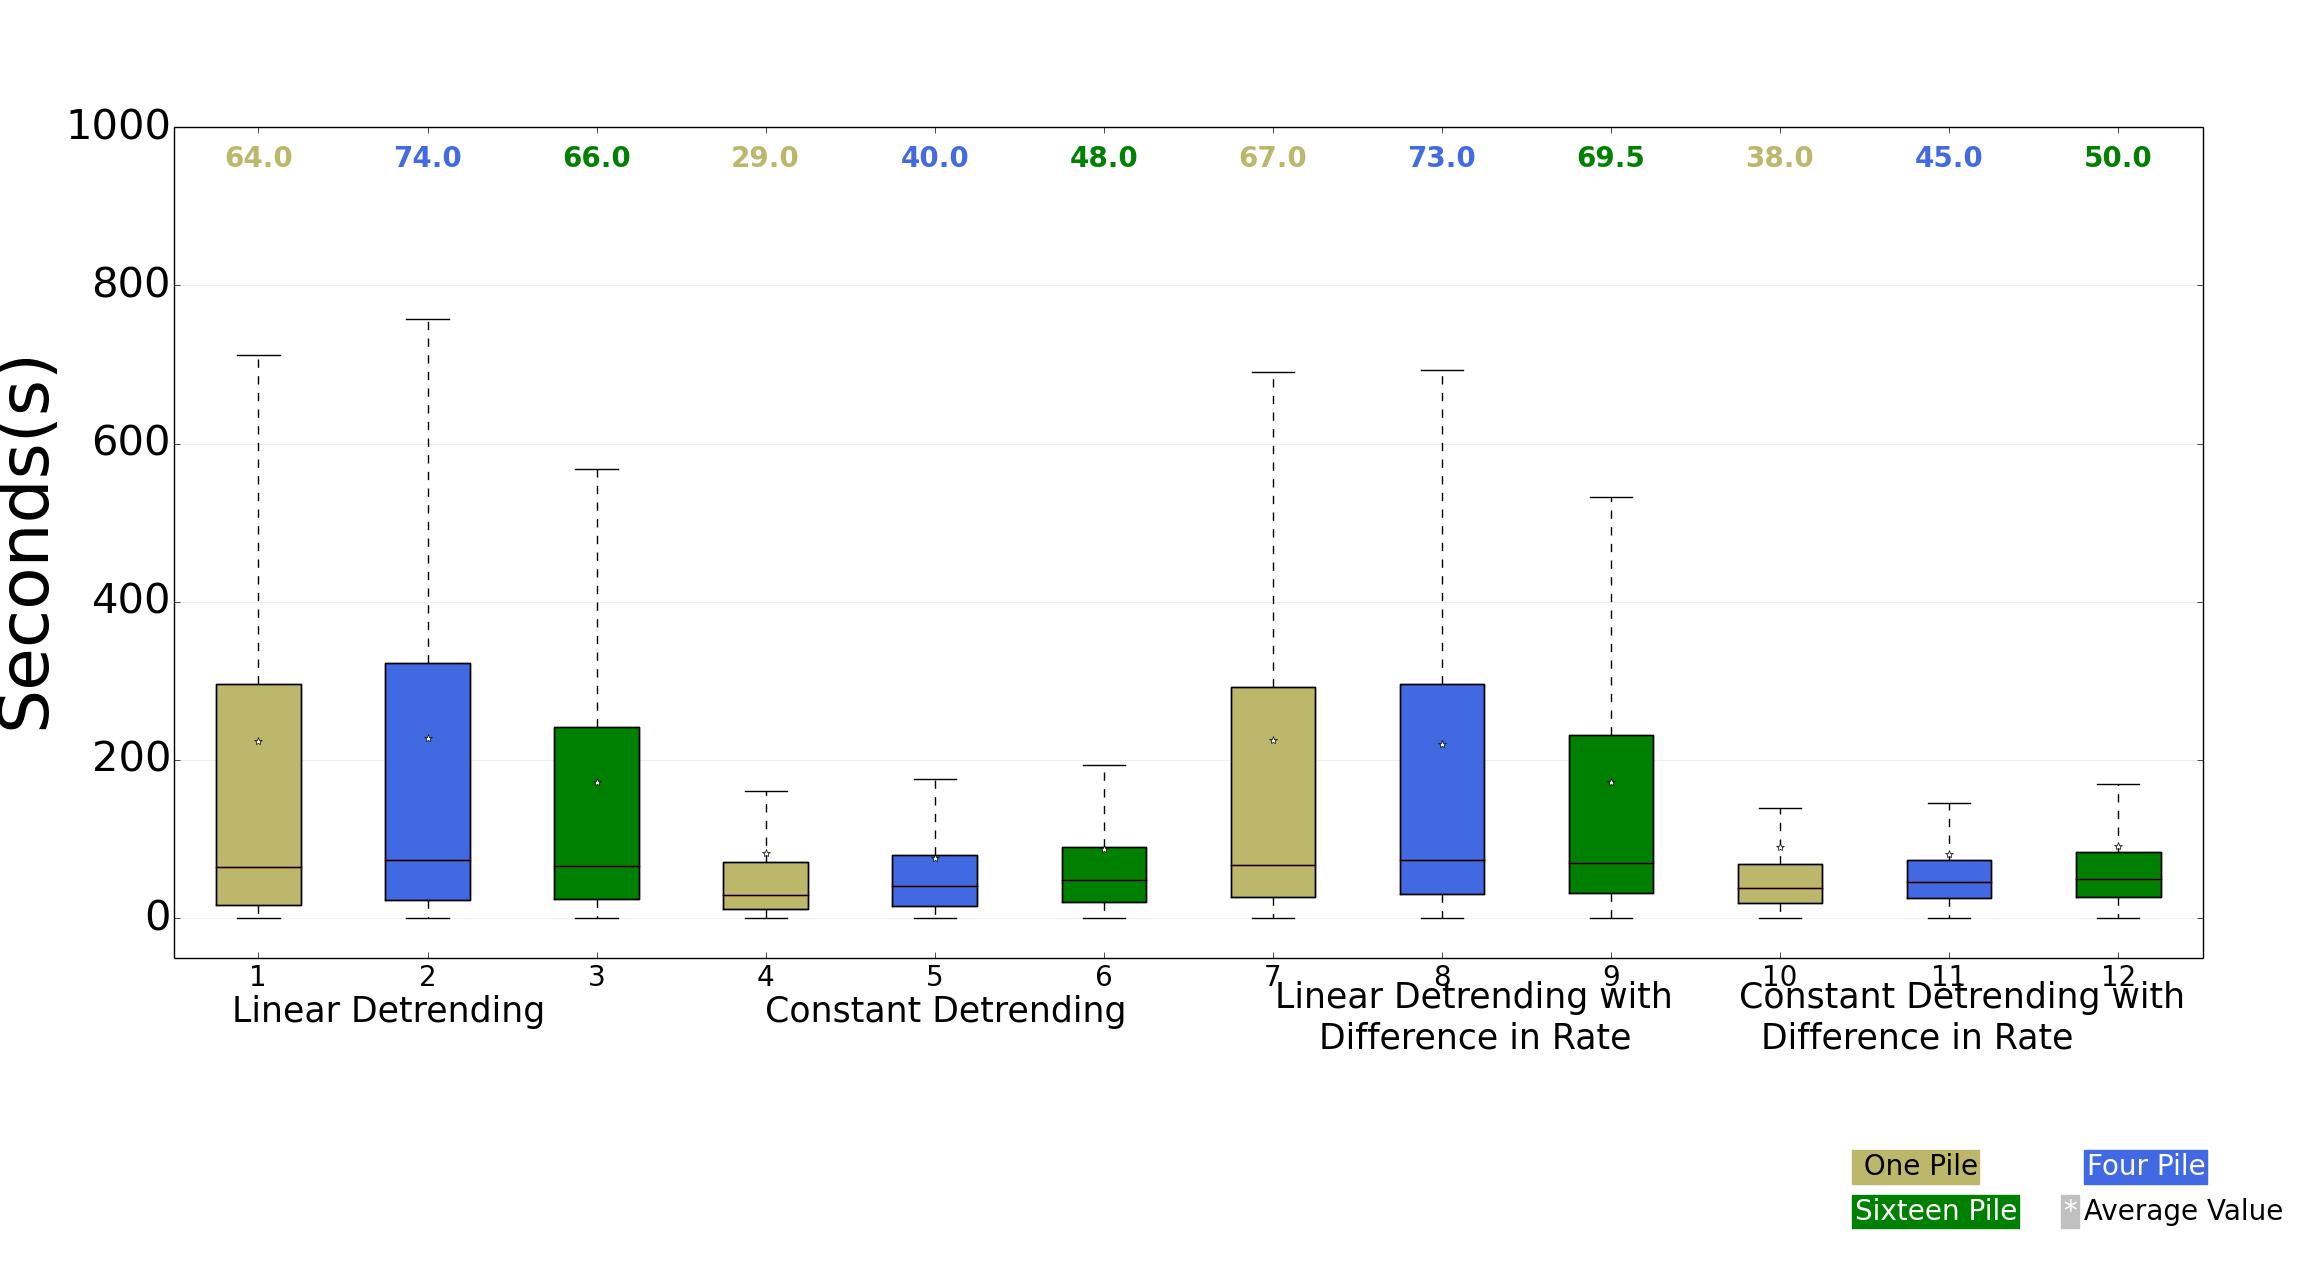
\includegraphics[width=\textwidth,height=0.35\textheight]{AllParameters/AllPlot.png}
	\caption{Comparison of all methods without outliers on data of \textit{P. Rugosus} for both combination of communication and memory}
\end{figure}
\begin{figure}
	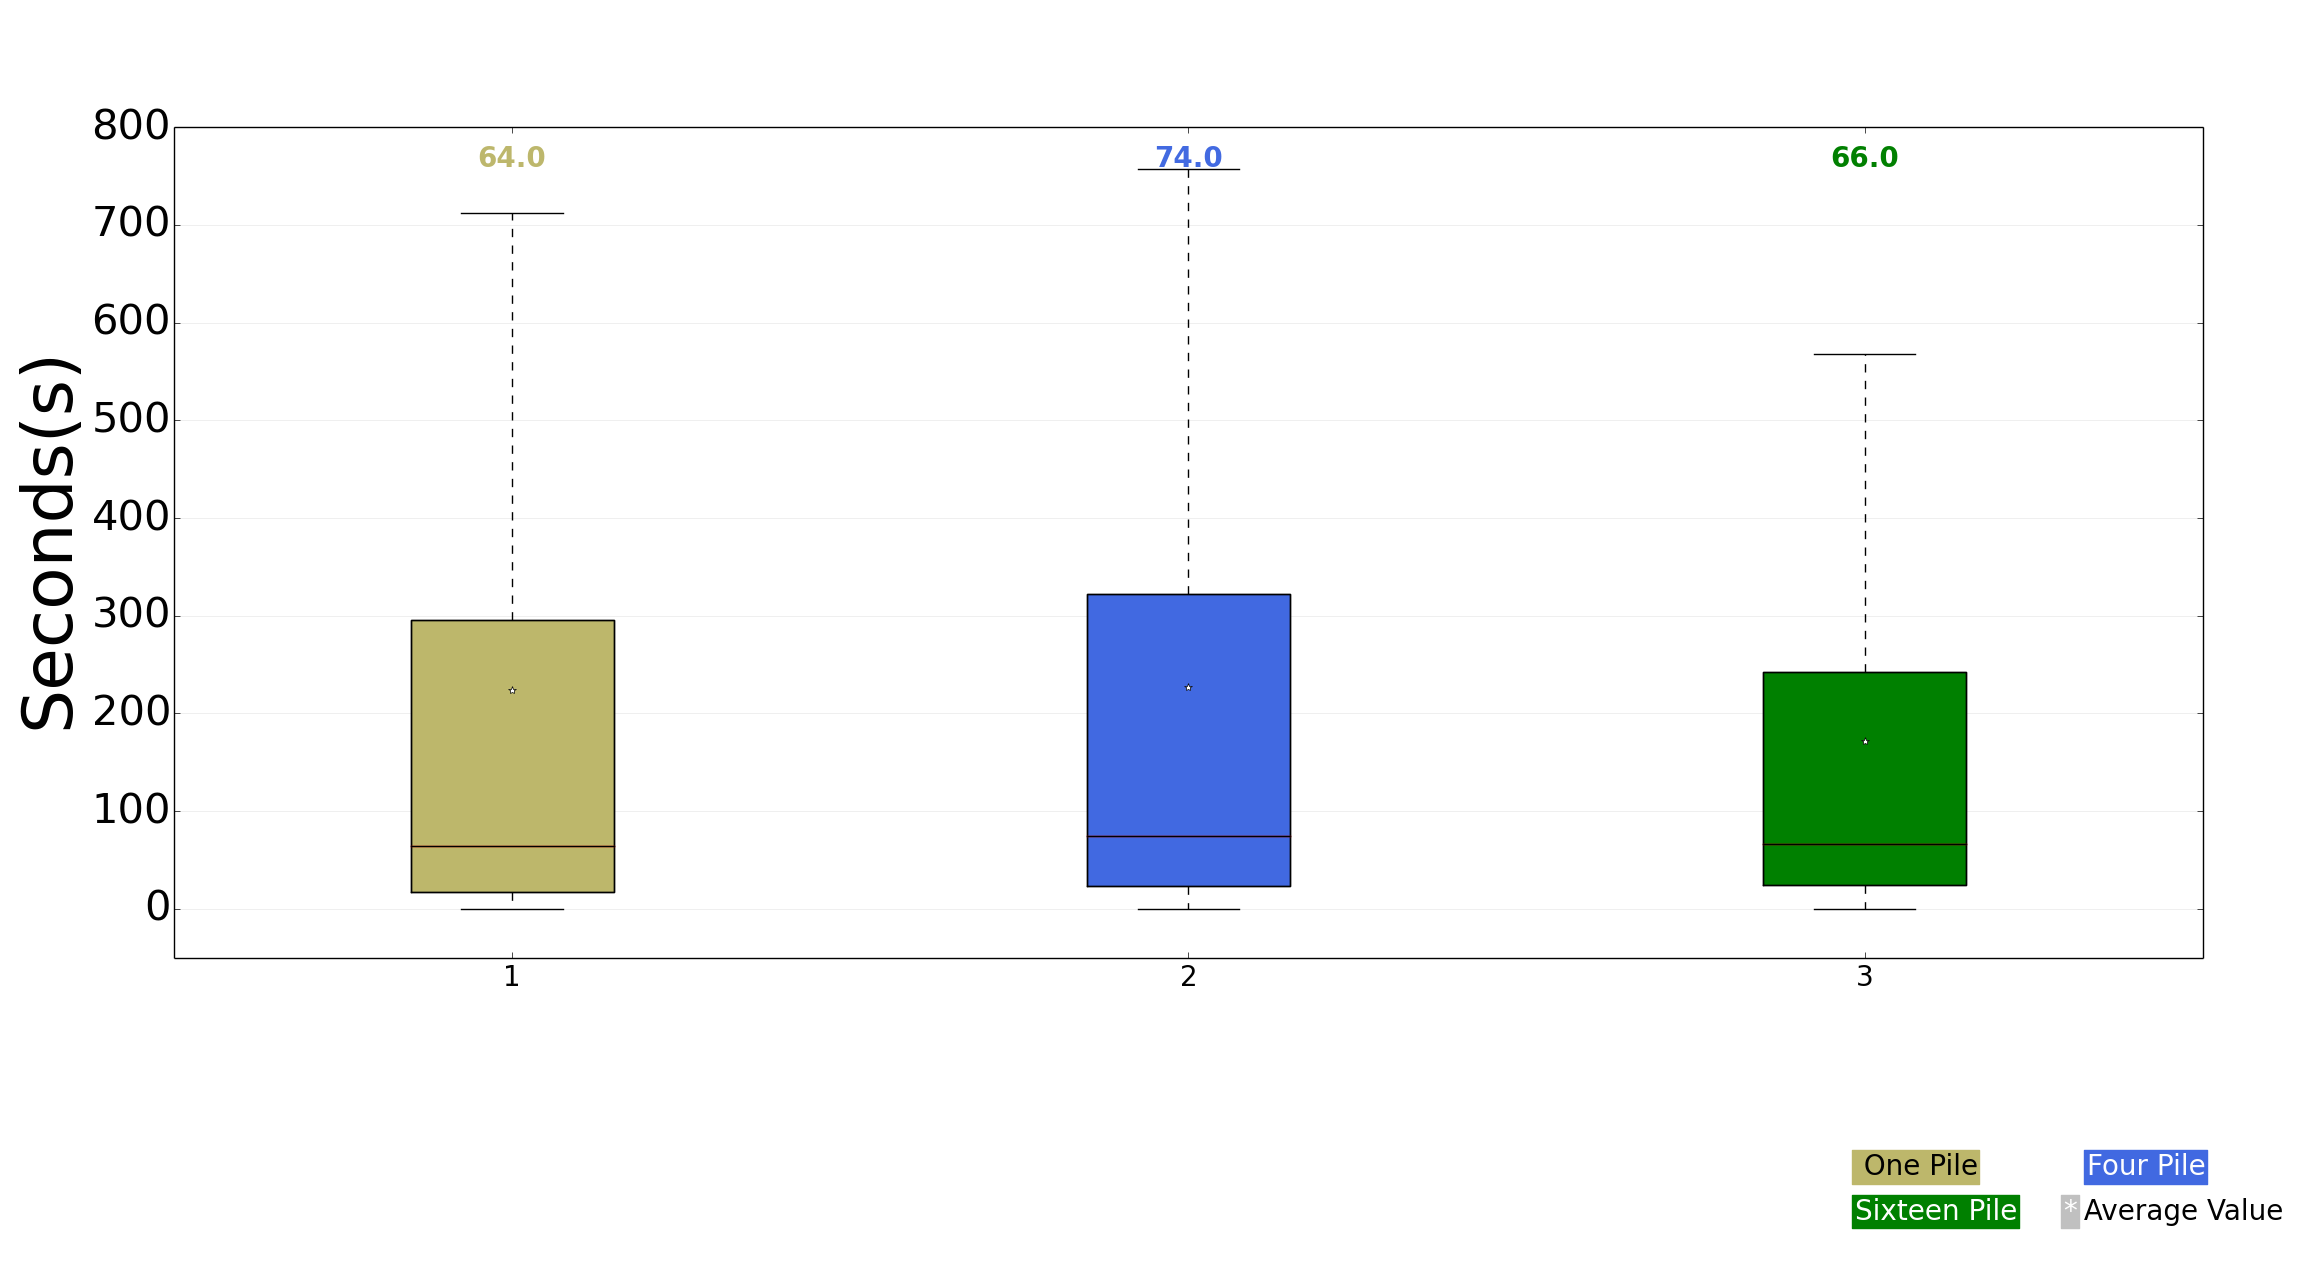
\includegraphics[width=\textwidth,height=0.35\textheight]{AllParameters/LinearDetrendingNoOutlier.png}
	\caption{Efficiency of linear detrending on data of \textit{P. Rugosus} for combination of communication and sitefidelity }
\end{figure}
\begin{figure}
	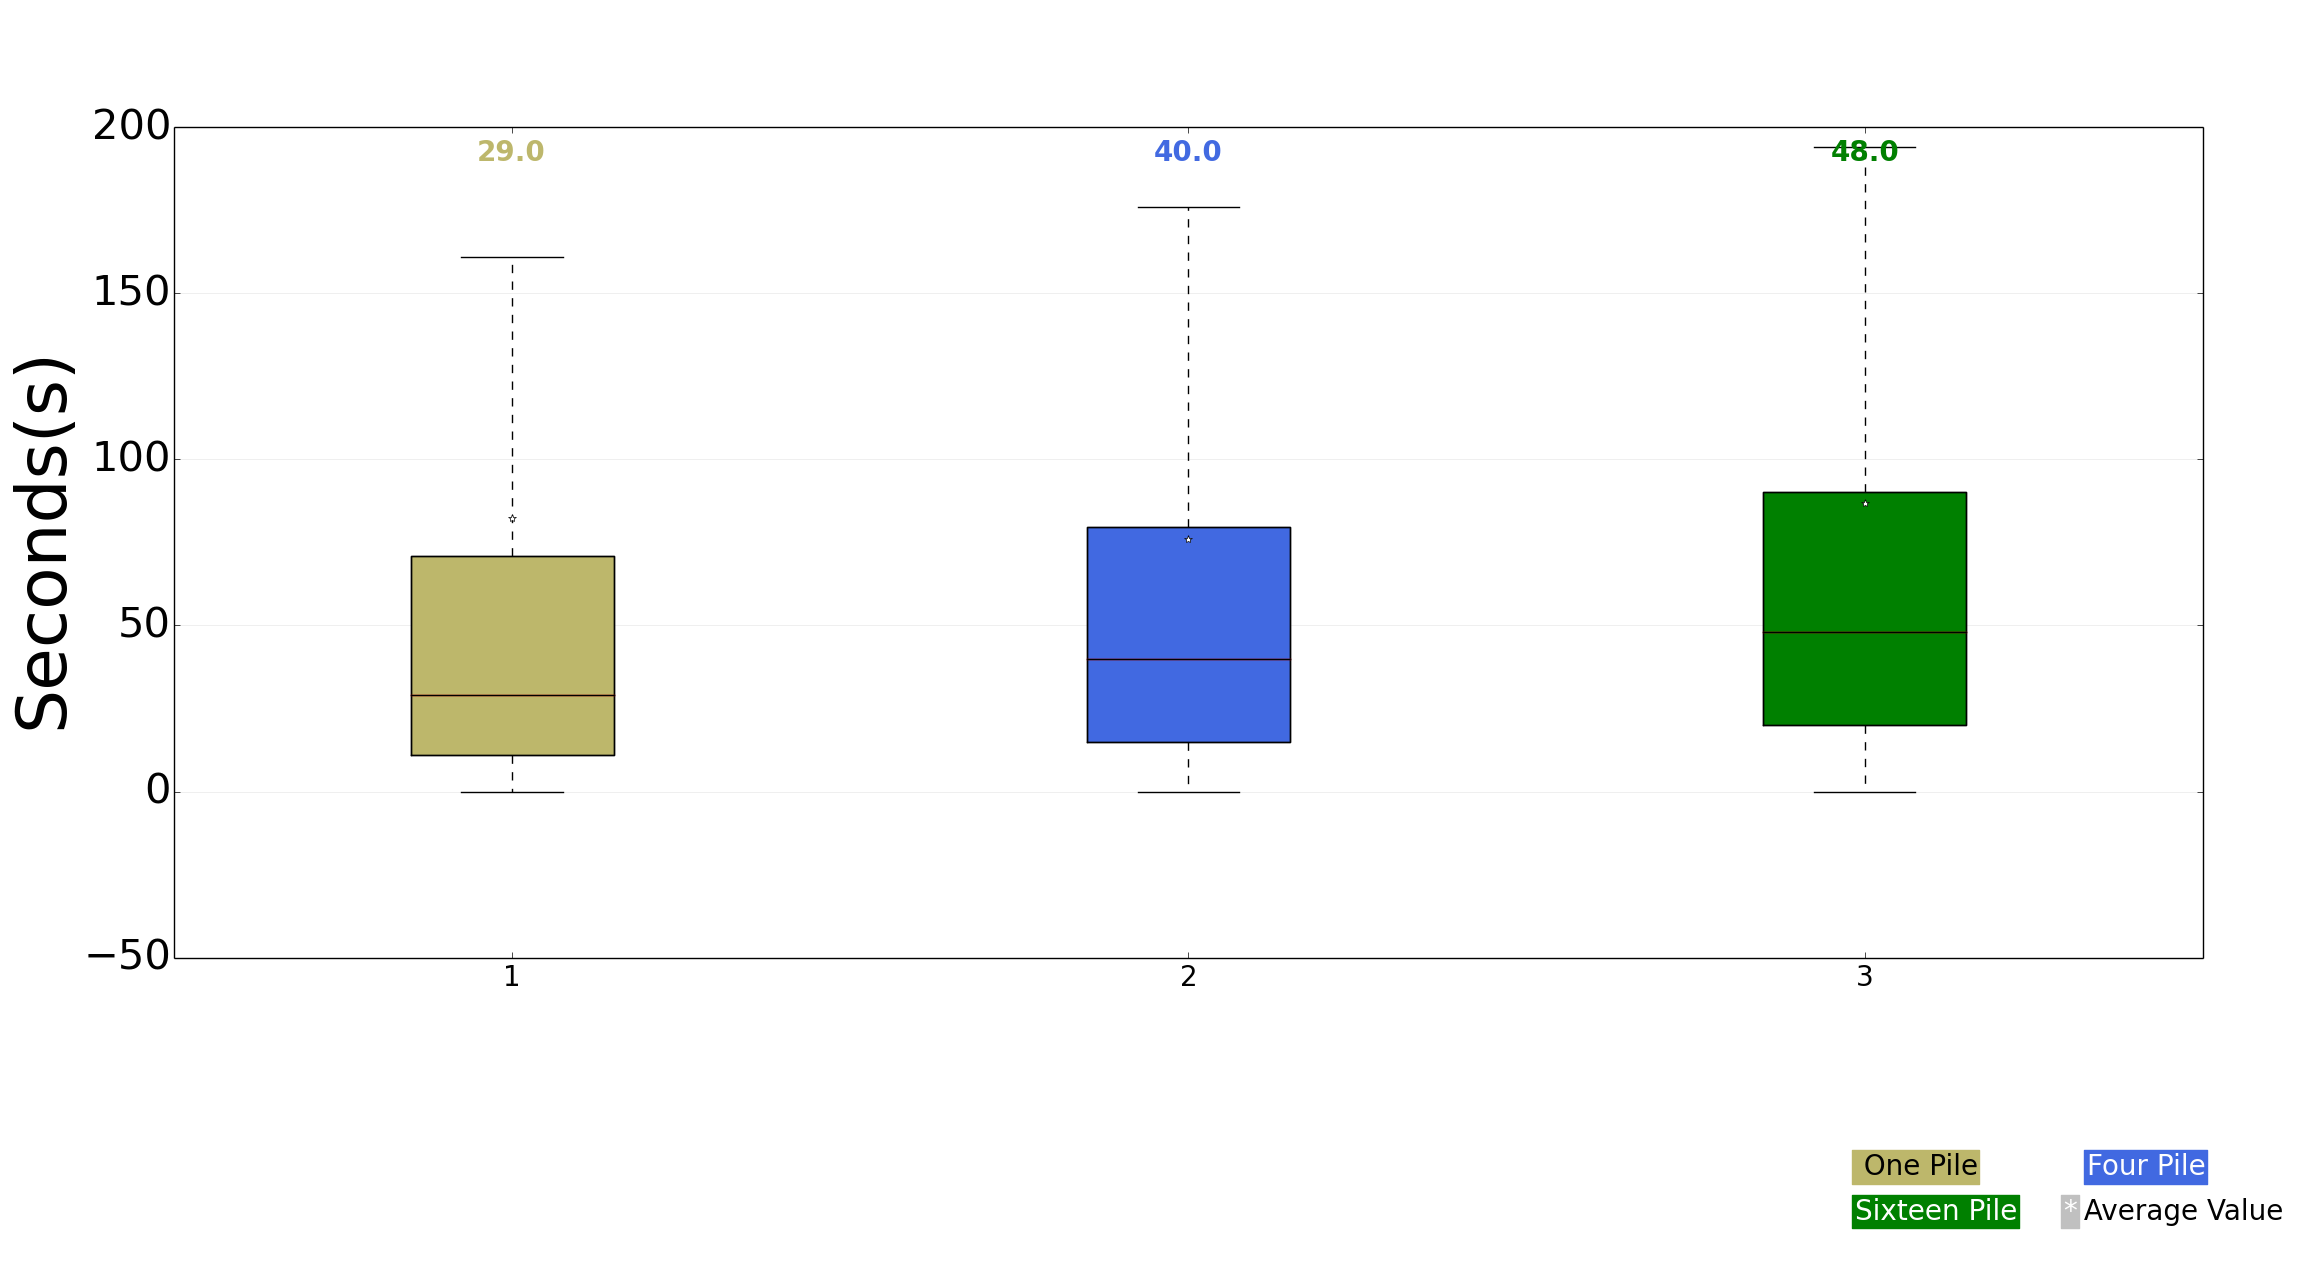
\includegraphics[width=\textwidth,height=0.35\textheight]{AllParameters/ConstantDetrendingNoOutlier.png}
	\caption{Efficiency of constant detrending methods on data of \textit{P. Rugosus} for both combination of communication and memory}
\end{figure}
\begin{figure}
	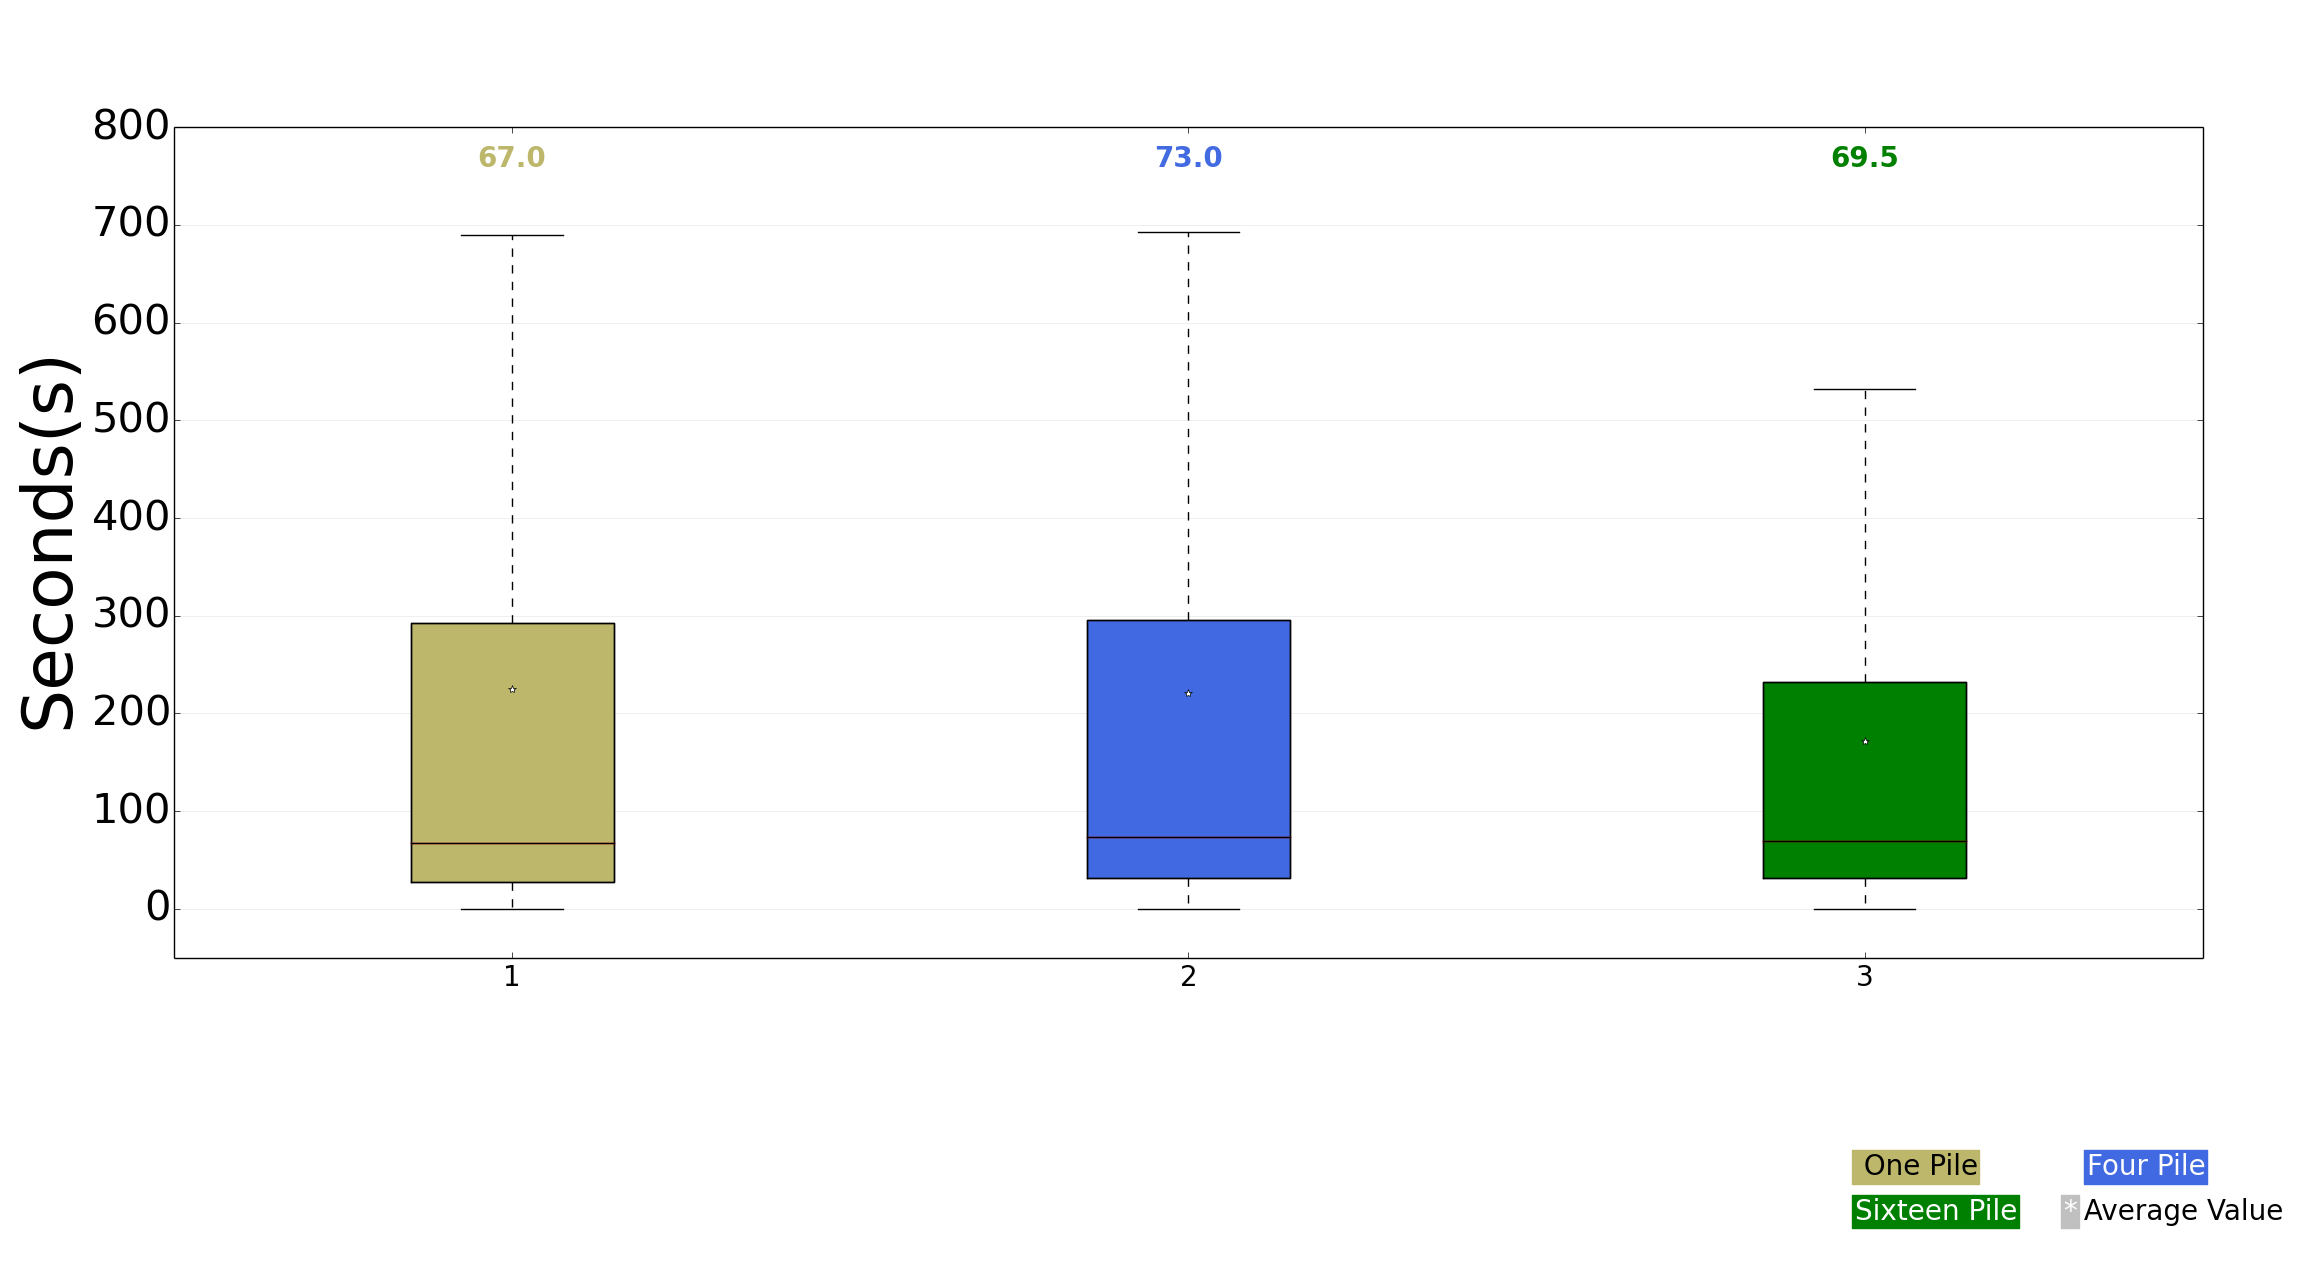
\includegraphics[width=\textwidth,height=0.35\textheight]{AllParameters/LinearDetrendingNoOutlierRateOfChange.png}
	\caption{Efficiency of linear detrending method with rate of change in foraging rate on data of \textit{P. Rugosus} for both combination of communication and memory}
\end{figure}
\begin{figure}
	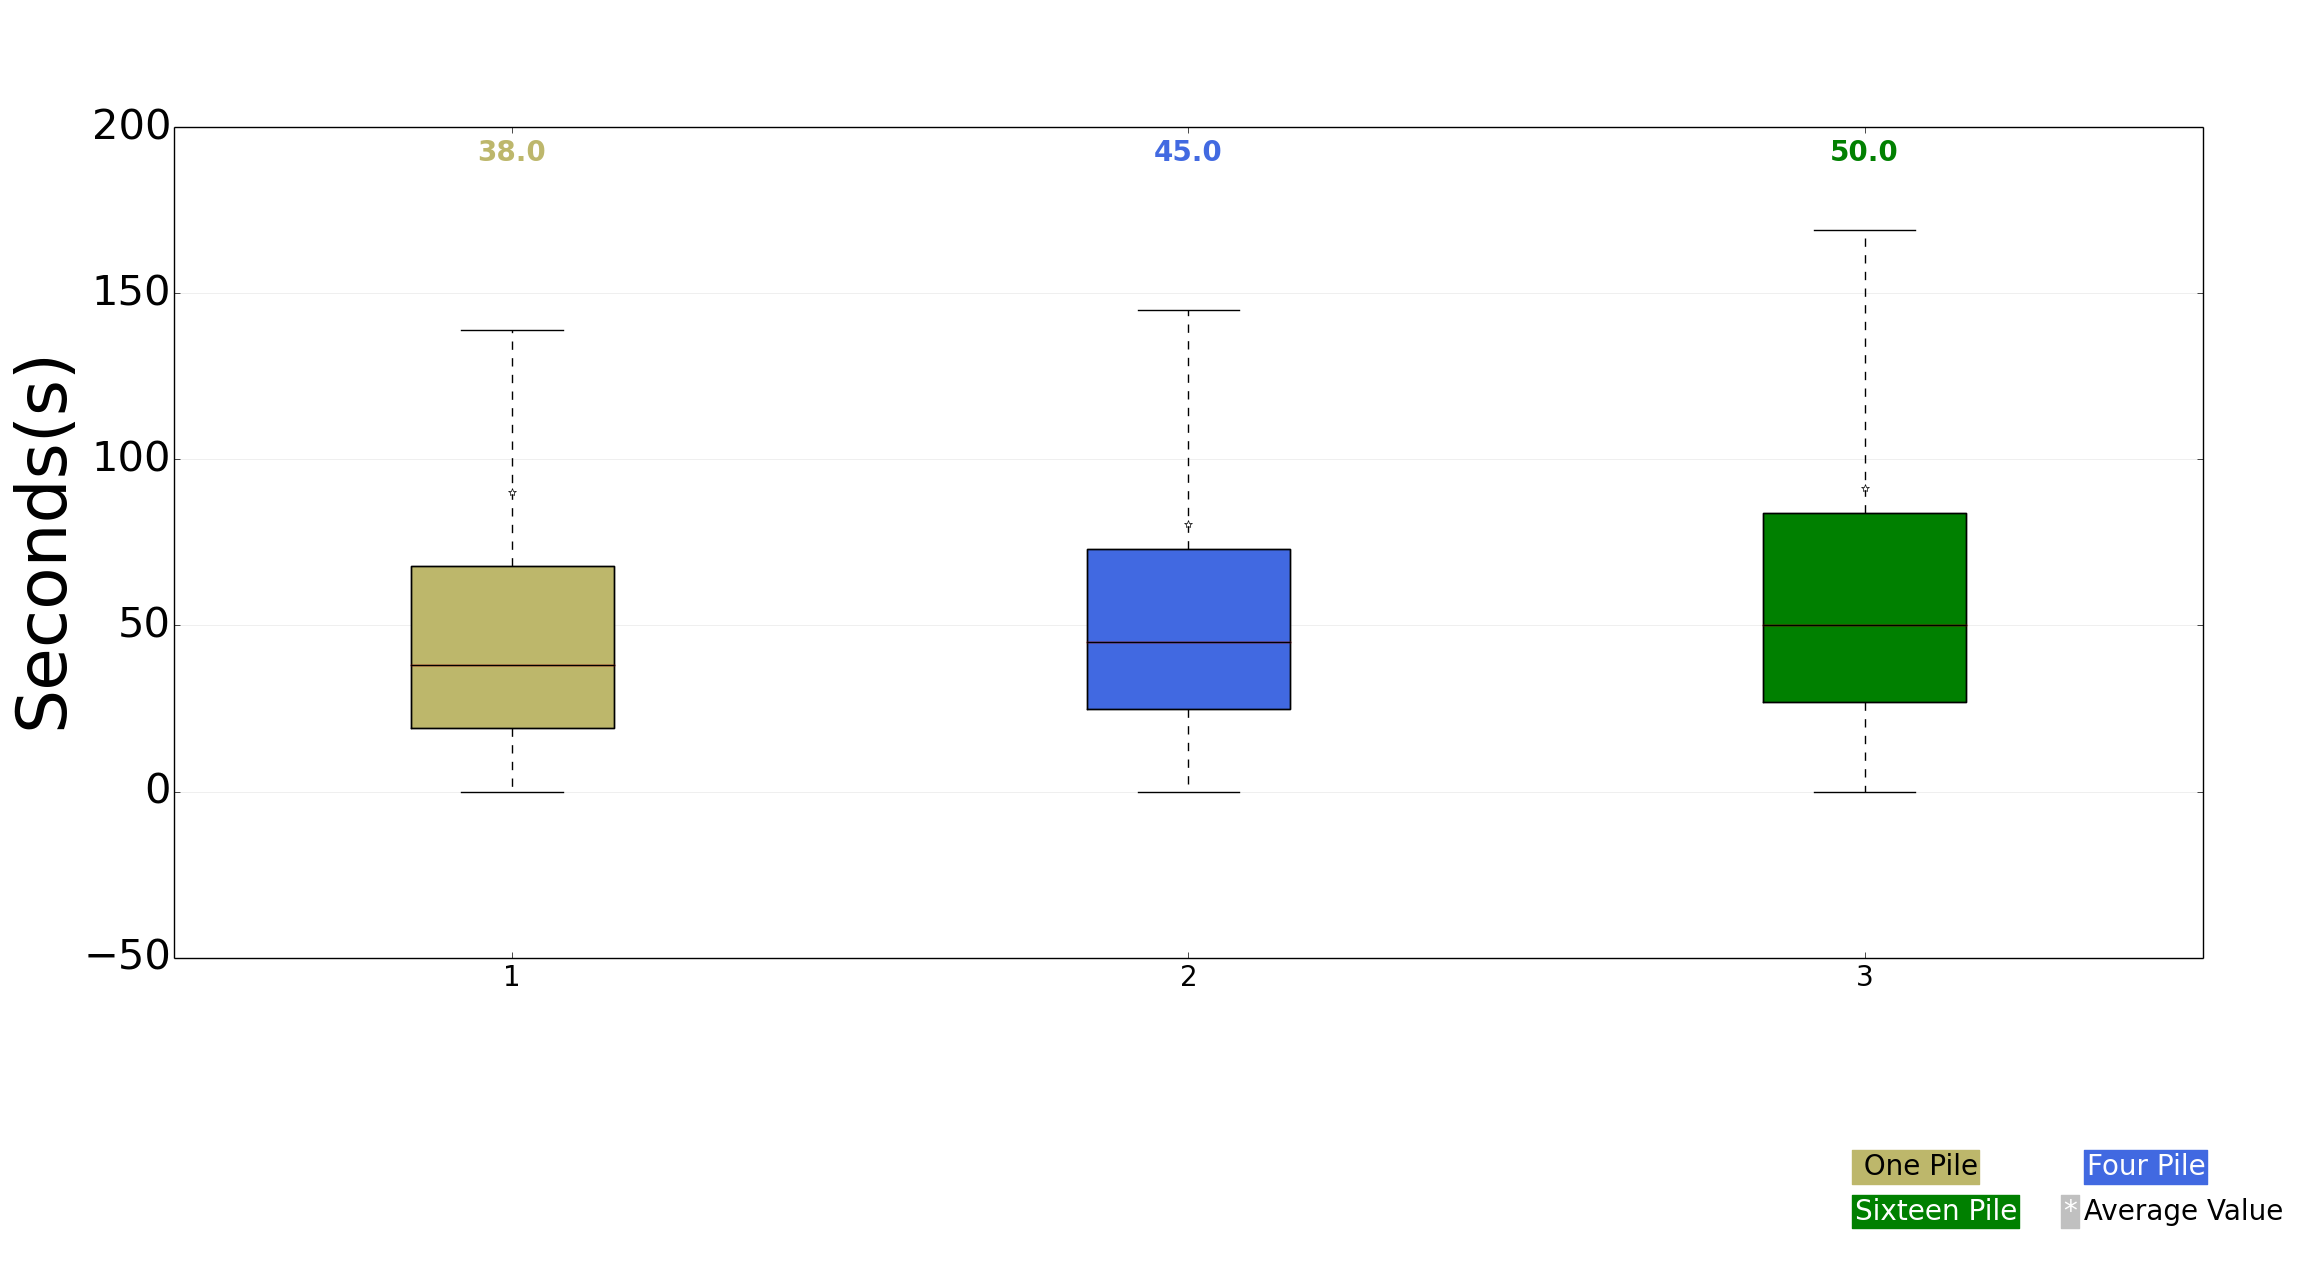
\includegraphics[width=\textwidth,height=0.35\textheight]{AllParameters/ConstantDetrendingNoOutlierRateOfChange.png}
	\caption{Efficiency of constant detrending method with rate of change in foraging rate on data of \textit{P. Rugosus} for both combination of communication and memory}
\end{figure}
\begin{figure}
	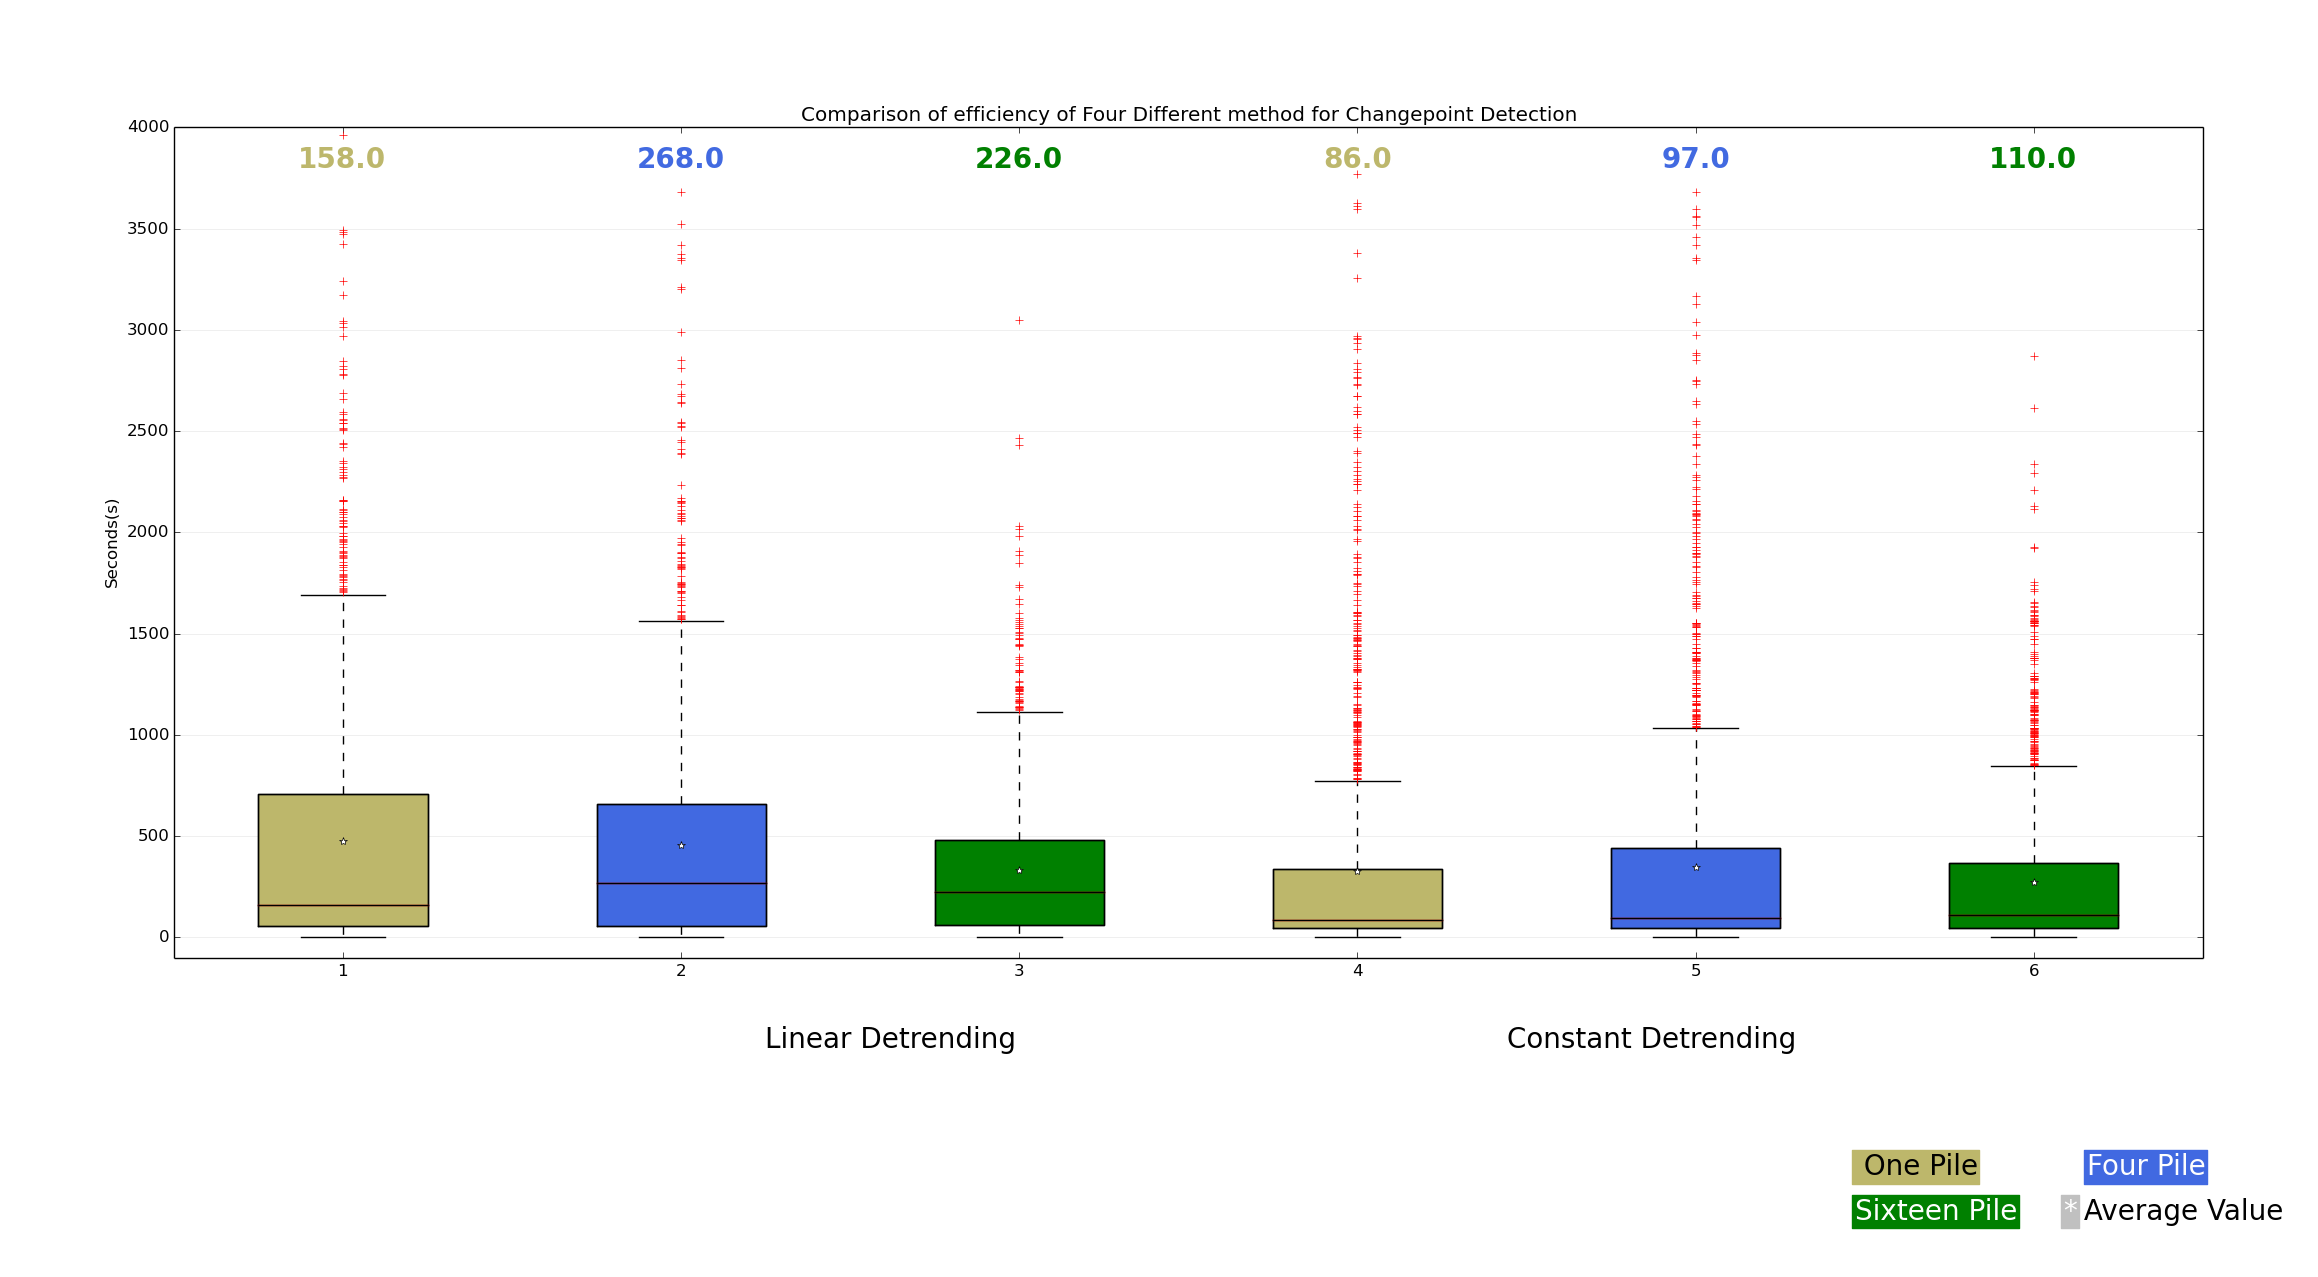
\includegraphics[width=\textwidth,height=0.35\textheight]{SiteFidelityOnly/SiteFidelity_2.png}
	\caption{Comparison of all methods on data of \textit{P. Rugosus} for memory only parameters}
\end{figure}
\begin{figure}
	\includegraphics[width=\textwidth,height=0.35\textheight]{SiteFidelityOnly/SiteFidelity_WithoutOutlier_2.png}
	\caption{Comparison of all methods without outliers on data of \textit{P. Rugosus} for memory only parameters}
\end{figure}


\bibliographystyle{plain}
\bibliography{bibfile_name}

\end{document}
